\documentclass[fontsize=10pt,paper=b5,open=any,
twoside=yes,toc=listof,toc=bibliography,headings=optiontohead,
captions=nooneline,captions=tableabove,english,DIV=15,numbers=noenddot,final,parskip=half-,
headinclude=true,footinclude=false,BCOR=.5cm]{scrbook}
\pdfvariable suppressoptionalinfo 512\relax
\usepackage[bottom]{footmisc}
\raggedbottom
\usepackage{lualatex-math}
\usepackage{wrapfig2}
\usepackage{hirostyle}
\usepackage{hiromacros}

\newcommand{\figW}{\columnwidth}
\newcommand{\figH}{0.61803551232\figW}

\newcommand{\legendfontsize}{\tiny}
\newcommand{\tickfontsize}{\tiny}
\newcommand{\labelfontsize}{\scriptsize}


% \usepackage{verbatim} % provides the `\comment` block
% \renewenvironment{figure}[1][]{%
% \expandafter\comment%
% }{%
% \expandafter\endcomment%
% }
% \renewenvironment{wrapfig}[1][]{%
% \expandafter\comment%
% }{%
% \expandafter\endcomment%
% }


\addbibresource{references.bib} \synctex=1 \title{Accessing the Global
  Unitary Dynamics of Open Quantum Systems with the Hierarchy of Pure
  States} \author{Valentin Boettcher} \date{\today}

\begin{document}
\makeatletter
\thispagestyle{empty}
\begin{titlepage}
  \includegraphics[width=5cm]{figs/logo.pdf}
  \vspace{1em}
  \hrule

  {\centering
  \setstretch{1.1}
  \vspace*{5em}
  {\bfseries\Huge \@title\\}
  \vspace*{2em}
  {\Large\@subtitle}
    \vfill \vfill
    {\large {\bfseries Master-Arbeit} \\
      zur Erlangung des Hochschulgrades\\
      Master of Science (M.Sc.)\\
      im Master-Studiengang Physik}

    \vfill vorgelegt von \vspace{1em}

  {{\large \@author} \\
  geboren am 06.06.1998 in Gera}
  \vfill
  {\large Institut f\"ur Theoretische Physik\\
    Fakultät Mathematik und Naturwissenschaften\\
    Technische Universität Dresden \\}
}

\newpage \thispagestyle{empty}\ \newpage
\clearpage
\thispagestyle{empty}
\null\vfill
{\large Eingereicht am September 30, 2022}

\begin{tabular*}{.5\linewidth}[h]{ll}
  1. Gutachter: & Prof. Dr. Walter Strunz \\
  2. Gutachter: & Dr. Kimmo Louma \\
\end{tabular*}
\end{titlepage}
\makeatother

\paragraph{Abstract}

Motivated by questions of quantum thermodynamics, the possibility of
accessing bath related observables in a Hamiltonian system bath
model are explored.  Examples that will be explored within the
framework of the Non-Markovian Quantum State Diffusion (NMQSD) and its
numerical implementation, the Hierarchy of Pure States (HOPS) are the
expectation value of the interaction Hamiltonian and the change of the
bath energy expectation value.  It is shown that a consistent
computation of these observables is indeed possible through comparison
with an exact solution for quantum Brownian motion and by testing
energy conservation.  The developed formalism is subsequently applied
to study the energy transfer in the fundamental spin-boson model. Some
theoretical notions related to energy extraction from open systems
with thermal baths are highlighted and applied to guide the study of
energy extraction in a driven spin boson model and a quantum Otto
cycle.


\paragraph{Zusammenfassung}

Motiviert durch Fragen der Quanten-Thermodynamik wird die Möglichkeit
des Zugriffs auf badbezogene Observablen in einem Hamiltonschen
System-Bad Modell erforscht.  Beispiele, die im Rahmen der Rahmen der
Non-Markovian Quantum State Diffusion (NMQSD) und ihrer numerischen
Implementierung, der Hierarchy of Pure States (HOPS), untersucht
werden, sind der Erwartungswert des Wechselwirkungs-Hamiltonians und
die Änderung des Bad-Energie Erwartungswertes.  Durch durch Vergleich
mit einer exakten Lösung für ein quantenmechanisches Modell der
Brownschen Bewegung und durch Prüfung der Energieerhaltung wird
gezeigt, dass eine konsistente Berechnung dieser Observablen moeglich
ist.  Der entwickelte Formalismus wird anschließend angewandt um den
Energietransfer im fundamentalen Spin-Boson-Modell zu
untersuchen. Einige theoretische Begriffe im Zusammenhang mit der
Energiegewinnung aus offenen Systemen mit thermischen Bädern werden
vorgestellt und angewendet, um die Untersuchung der Energieextraktion
in einem getriebenen Spin-Boson-Modell und einem quantenmechanischen
Otto Prozess zu leiten.

\tableofcontents

% Chapters
\chapter{Introduction}
\label{chap:intro}
\begin{itemize}
\item this is not finished!! (not event close to being so)
\item motivate interesting thermodynamical questions and the advantage
  of the NMQSD/HOPS in this case without repeating \cref{sec:ergo_general}
\end{itemize}

The exact treatment of strongly coupled and non Markovian open quantum
systems is a challenging problem.  If no analytical solution is
available, numerical methods have to be relied upon. Notably there are
HEOM\fixme{cite more}.

Besides the reduced dynamics of the system, the field of quantum
thermodynamics has attracted much interest. Quantum thermodynamics is,
among other issues, concerned with extending the standard
phenomenological thermodynamic notions to microscopic systems coupled
to macroscopic baths. This setting may make it possible to make
rigorous microscopic definitions of thermodynamic quantities such as
internal energy, heat and work that are consistent with the laws of
thermodynamics. There is no consensus on this matter yet, as is
demonstrated by the plethora of proposals and discussions in
\cite{Rivas2019Oct,Talkner2020Oct,Motz2018Nov,Wiedmann2020Mar,Senior2020Feb,Kato2015Aug,Kato2016Dec,Strasberg2021Aug,Talkner2016Aug,Bera2021Feb,Bera2021Jun,Esposito2015Dec}.

As system and baths may not be regarded as completely separable
entities in a strong coupling
regime~\cite{Rivas2019Oct,Esposito2015Dec}, an insight into the
dynamics of the bath is crucial. In some settings
\cite{Kato2016Dec,Lobejko2021Feb, Strasberg2021Aug}, such as cyclic
heat engines, the change in the bath energies is a quite suitable
definition of heat, as is expounded in
\cref{sec:basic_thermo,sec:operational_thermo}.

As it turns out, the framework of the ``Non Markovian State
Diffusion'' (NMQSD)~\cite{Diosi1998Mar}, which will be reviewed
in~\cref{sec:open_systems}, allows access to certain bath related
observables such as the time derivative of the bath energy expectation
value and the interaction Hamiltonian expectation value. The

In \cref{sec:basic_thermo}, some operational quantum thermodynamical
questions will be discussed and some light will be shed on the
necessity of infinite baths.

\Cref{chap:flow} presents the main result of this thesis, namely
formulas to calculate expectation values of bath related
observables. Finally, we will discuss some numerical applications of
the result in \cref{chap:numres}. These application include a
\fixme{references}.

In \cref{chap:hops_notes}, some HOPS related subjects are discussed,
including a derivation of the HOPS for multiple baths embedded in an
auxiliary bosonic Fock space in \cref{sec:multihops}.

\newpage

\section{Open Quantum Systems}
\label{sec:open_systems}
Quantum physics' most important equation, the Schr\"odinger equation,
allows us to predict the future of a system knowing its initial
state. Writing it down
\begin{equation}
  \label{eq:schroedinger}
  \iu ∂_{t} \ket{ψ(t)} = H \ket{ψ(t)},
\end{equation}
we find that we need to specify a \emph{Hamiltonian} \(H\) that acts
on our system state which is an element of a Hilbert space of some
dimension \(N\). Throughout the work we set \(\hbar=c=1\).

We call the time evolution generated by \cref{eq:schroedinger}
\emph{Unitary}, as it preserves the norm of a state and is reversible.
Given any time independent Hamiltonian we may write down the time
evolution operator to solve the Schr\"odinger equation
\begin{equation}
  \label{eq:time_evo_op}
  U(t, t_{0})=\eu^{-\iu H (t-t_{0})},\; U(t, t_{0})^\dag U(t, t_{0}) =
  \id,\; U\ket{ψ(t_{0})} = \ket{ψ(t)}.
\end{equation}

For time independent Hamiltonians the Schr\"odinger equation describes
a closed system which constitutes, within the scope of the problem in
question, the whole universe. In general, it is very hard to find a
closed expression for \cref{eq:time_evo_op}, except for very special
cases. Either one takes to approximations or one applies numerical
methods to solve \cref{eq:schroedinger}.

When the Hilbert space dimension is small, its numerical solution is
straight forward. But in more realistic scenarios we may still be
interested in a small system, but we cannot neglect the interaction of
that system with a much larger environment sometimes consisting of
infinite degrees of freedom. If the atmosphere of the earth would be
neglected when describing the descent of a space reentry capsule we
would arrive at fatally wrong results. Similarly, modern applications
of quantum physics deal with systems that undergo quantum evolution
under conditions that are not consistent with an isolated
system. Specifically in quantum computing~\cite{Gill2022Jan} the
effect of environmental interactions poses a major problem.

As a classical example, stokes drag models the influence of a viscous
fluid on spherical objects and can be implemented by adding a velocity
dependent term to the equation of motion of our object,
\begin{equation}
  \label{eq:newton}
  \ddot{x} = F - α \dot{x}.
\end{equation}
We still retain all information about the system, the particle, having
accounted effectively for an environment, the fluid.

In quantum physics, we find that the situation is more complicated.
Writing down a Hamiltonian we have to account for both system and
environment in a composite Hilbert space \(\hilb=\hilb_{\sys}\otimes\hilb_{\bath}\)
\begin{equation}
  \label{eq:general_open}
  H = H_{\sys} \otimes \id_{\bath} + \id_{\sys} \otimes H_{\bath} + H_{\inter},
\end{equation}
where \(\sys\) marks the system, \(\bath\) marks the environment (or
bath) and \(H_{\inter}\) models the environment.

Although the global state of system and environment may be pure,
entanglement of system and environment leads to the effect, that we
may know the system state only as a statistical mixture of states
called the \emph{reduced state}. No part of a composite system may be
in general be known as ``precicely'' as the whole.

Starting from a possibly mixed global state \(ρ(t)\) we find, that to
find the dynamics of all observables \(O_{\sys}\) that only act on the
system Hilbert space it is sufficient to know
\(ρ_{\sys}(t)=\tr_{\bath}[ρ(t)]\), the reduced system state.

The partial trace \(\tr_{\bath}\) averages over all bath degrees of
freedom and removes them from explicit consideration. This is a most
useful device, as the environment usually has a Hilbert space
dimension that is much too large for practical
calculations. Especially in numerically this fact is important, as
even an environment consisting of \(50\) two level systems would
consume \(128\) tebibyte of memory when stored as double precision
floating point numbers.

Under certain assumptions, most importantly that of weak coupling
\(\ev{H_{\inter}}\approx 0\), a pertubative treatment of the
environment yields an evolution equation, called a \emph{master
  equation}, that only contains the system state
\(ρ_{\sys}\)~\cite[p. 115 ff.]{Breuer2002Jun,Rivas2012}. This equation
often called Gorini–Kossakowski–Sudarshan–Lindblad equation, or GKSL
equation in short, leads to irreversible non unitary dynamics and has
the form
\begin{equation}
  \label{eq:gksl}
  \dot{ρ}_{\sys} = -\iu \comm{H}{ρ_{\sys}} + \mathcal{D}[ρ_{\sys}] = \mathcal{L}[ρ_{\sys}],
\end{equation}
where \(\mathcal{D}\) is called the \emph{dissipator} which adds
non-unitary dynamics to the von Neumann equation and \(H\) is a
unitary contribution not necessarily equal to \(H_{\sys}\).

Integrating \cref{eq:gksl} leads to a map
\(ρ_{\sys}(t) = \mathcal{E}_{t}(ρ_{\sys}(0))\).  The evolution
generated \cref{eq:gksl} is called Markovian, as
\(\mathcal{E}_{t+s}= \mathcal{E}_{t}\circ\mathcal{E}_{s}\). More
fundamentally, this due to the fact that one at some point assumes,
that the bath has no ``memory''\footnote{This does not mean that the global
state has always the form \(ρ_{\sys}(t)\otimes
ρ_{\bath}(t)\)~\cite{Rivas2012}.}. Without getting into the details,
one may say that the characteristic time scales upon which correlation
functions of bath observables decay should be much smaller than the
time scales of the system.

If one endeavors to drop the assumptions of weak coupling and of
Markovian dynamics, the situation becomes more complicated. But when
introducing a concrete model of the bath we find that
\cref{eq:schroedinger} can be recast into a form that allows for an
exact numerical solution. The great advantage from the standpoint of
this thesis is, that although we solve for the reduced state
\(ρ_{\sys}\), we essentially calculate the unitary dynamics of system
and bath retain some information about the bath. This allows to
quantify the change in expected bath energy and also the expectation
value of the interaction Hamiltonian.

\Cref{sec:nmqsd_basics} will introduce the general model whose
solution will be made feasible with the introduction of the \emph{Non
  Markovian Quantum State Diffusion} (NMQSD). The numerical
implementation of the NMQSD, the \emph{Hierarch of Pure States}
(HOPS), will be the topic of \cref{sec:hops_basics}.

A more detailed account of both subjects can be found in
\cref{sec:multihops} as well as \cite{RichardDiss}.


The basics of the NMQSD will be briefly reviewed in
\cref{sec:nmqsd_basics} as will the basics of HOPS in
\cref{sec:hops_basics}.

\section{The Non Markovian Quantum State Diffusion}
\label{sec:nmqsd_basics}

We will now introduce the fundamental form of the models that will be
discussed in this thesis. This model has a wide applicability and many
microscopic systems can be cast into its form
\cite{Strunz2001Habil}\cite[chap. 2]{RichardDiss}, although there
certainly exist limits of applicability~\cite{Caldeira2014Mar}.

Consider a general quantum system \(H_\sys(t)\) coupled to \(N\) baths
of harmonic oscillators\footnote{For instance, the electromagnetic field.}
\begin{equation}
  \label{eq:generalmodel}
  H(t) = H_\sys(t) + ∑_{n=1}^N \qty[L_n^†(t)B_n + \hc] + ∑_{n=1}^NH_B\nth ,
\end{equation}
with \(B_n=∑_{λ} g_λ\nth a_λ\nth\) and
\(H_B\nth=∑_λω_λ\nth \qty(a_λ\nth)^\dag a_λ\nth\). The \(a_λ\) are
bosonic annihilation operators and the \(L_n\) are arbitrary not
necessarily hermitian operators system Hilbert space.

Despite the simple structure of the baths, \cref{eq:generalmodel} is
generally very hard to solve beyond weak coupling strengths as has
been detailed in~\cref{sec:open_systems}. The ``Non Markovian Quantum
State Diffusion'' (NMQSD)~\cite{Diosi1998Mar} approach allows to
recast \cref{eq:generalmodel} into a stochastic differential equation
in which the bath degrees of freedom are accounted for by Gaussian
stochastic processes.

Here we only consider a single zero temperature bath initially in the
ground state \(\ket{0}\). For more complete and general account see
\cite{RichardDiss,Strunz2001Habil,Diosi1998Mar,Hartmann2017Dec} and
\cref{sec:hops_multibath}.

The total system-bath state may then be expanded in a Bargmann
coherent state basis~\cite{klauder1968fundamentals} with respect to
the bath degrees of freedom
\begin{equation}
  \label{eq:projected_single}
  \ket{ψ(t)} = ∫{\frac{\dd{\vb{z}}}{π^{N}}\eu^{-\abs{\vb{z}}^2}}\ket{ψ(t,\vb{z})^\ast}\ket{\vb{z}},
\end{equation}
where \(\vb{z}\) is a vector of coherent state labels \(z_λ\) for each
environment oscillator.

After transforming \cref{eq:generalmodel} into the interaction picture
with respect to \(H_B\) and using the properties of the coherent
states (\(\mel{z_λ}{a_λ}{ψ}\rightarrow ∂_{z_λ^\ast}\braket{z_λ}{ψ}\),
\(\mel{z_λ}{a_λ^\dag}{ψ}\rightarrow z_λ^\ast\braket{z_λ}{ψ}\)) we
arrive at an equation for stochastic pure state trajectories
\begin{equation}
  \label{eq:nmqsd_single}\tag{NMQSD}
  ∂_tψ_t(η^\ast_t) = -\iu H ψ_t(η^\ast_t) +
  L {η}^\ast_tψ_t({η}^\ast_t) - L^†∫_0^t\dd{s}α(t-s)\fdv{ψ_t({η}^\ast_t)}{η^\ast_s},
\end{equation}
where \(α\) is the zero temperature bath correlation function (BCF)
\begin{equation}
  \label{eq:bcfdef}
  α(t-s) = \ev{B(t)B(s)} = ∑_λ \abs{g_λ}^2\,\eu^{-\iu ω_λ (t-s)}
\end{equation}
and \(η_t\) is a Gaussian stochastic process obeying
\begin{equation}
  \label{eq:single_processescorr}
  \begin{aligned}
      \mathcal{M}(η_t) &=0, & \mathcal{M}(η_tη_s) &= 0,
      & \mathcal{M}(η_tη_s^\ast) &= α(t-s).
  \end{aligned}
\end{equation}

The reduced system state may then be recovered by averaging over all
trajectories
\begin{equation}
  \label{eq:recover_rho}
  ρ_{\sys}(t) = \mathcal{M}_{η_{t}^\ast}\bqty{ψ_t(η_t)^\dag ψ_t(η^\ast_t)}.
\end{equation}

Note that the BCF \(α\) is usually defined as Fourier transform of the
spectral density
\begin{equation}
  \label{eq:specdens}
  J(ω) = {π} ∑_λ \abs{g_λ}^2 δ(ω-ω_λ).
\end{equation}
One then usually performs a continuum limit so that \(J(ω)\) becomes
``smeared out'' to a smooth function and \(α(τ)\) decays to zero for
\(τ\rightarrow ∞\).

We have found that indeed we can treat an infinite environment with a
stochastic differential equation in which only objects of system
dimension appear. Note also, that we can treat explicit time
dependence of \(L\) and \(H\) without alteration to
\cref{eq:nmqsd_single}.


The equation \cref{eq:nmqsd_single} does not preserve the norm of the
state, leading to suboptimal convergence of \cref{eq:recover_rho}.
To remedy this, we choose a co-moving shifted stochastic process
\begin{equation}
  \label{eq:shifted_proc}
  \tilde{η}_{t}^\ast= η^\ast_{t} + ∫_{0}^{t}\dd{s} α^\ast(t-s) \ev{L^\ast}_{s},
\end{equation}
where
\(\ev{L^\dag}_{t}=ψ(\tilde{η}_{t}^\ast)_{t}^\dag L^\dag
ψ(\tilde{η}_{t}^\ast)_{t}\).

This leads to the nonlinear NMQSD equation
\begin{equation}
  \label{eq:nmqsd_nonlin_single}
  ∂_tψ_t(η^\ast_t) = -\iu H ψ_t(η^\ast_t) +
  L {η}^\ast_tψ_t(\tilde{η}^\ast_t) - \pqty{L^† -\ev{L^\dag}_{t}}∫_0^t\dd{s}α(t-s)\fdv{ψ_t({η}^\ast_t)}{\tilde{η}^\ast_s}.
\end{equation}
There is a subtlety concerning the functional derivative that won't be
discussed here, but in \cref{sec:nonlin}.
Crucially, the system state is now recovered through
\begin{equation}
  \label{eq:recover_rho_nonlinear}
  ρ_{\sys}(t) = \mathcal{M}_{η_{t}^\ast}\bqty{\frac{ψ_t(η_t)^\dag ψ_t(η^\ast_t)}{\norm{ψ_t(η_t)}^{2}}},
\end{equation}
so that all trajectories contribute with ``equal weight''.


\section{The Hierarchy of Pure States}
\label{sec:hops_basics}
The equation \cref{eq:nmqsd_single} has removed the bath degrees of
freedom from explicit consideration, replacing them with a Gaussian
stochastic process and a rather complicated term containing a memory
integral and a functional derivative
\begin{equation}
  \label{eq:complicated_term}
  ∫_0^t\dd{s}α(t-s)\fdv{ψ_t({η}^\ast_t)}{η^\ast_s}.
\end{equation}

There exist analytical approaches to this
term~\cite{Diosi1998Mar,Strunz2001Habil}, but we keep the approach as
general as possible and instead choose a numerical avenue.

They key is define away the complicated term containing the functional
derivative as an auxiliary state. Expanding the BCF into exponentials
\(α(τ)=∑_{μ}G_{μ=1}^{M}\eu^{-W_{μ}τ}\) and defining
\begin{equation}
  \label{eq:d_op_one}
  D_{μ}(t)\equiv ∫_{0}^{t} G_{μ} \eu^{-W_{μ}(t-s)} \fdv{η^\ast_s},\; D^{\vb{k}}(t)\equiv Π_{μ=1}^{M}\sqrt{\frac{k_{μ}!}{G_{μ}^{k_{μ}}}}
  \frac{1}{i^{k_{μ}}}\pqty{D_{μ}}^{k_{μ}}
\end{equation}
we can define the \(\vb{k}th\) hierarchy state
\begin{equation}
  \label{eq:d_op_hier}
   ψ^{\vb{k}}\equiv D^{\vb{k}}ψ.
\end{equation}

For this state the following equation of motion can be derived
\begin{equation}
  \label{eq:singlehops}\tag{HOPS}
  \dot{ψ}^{\vb{k}} = \qty[-\iu H_\sys + \vb{L}\cdot\vb{η}^\ast -
  ∑_{μ=1}^{M}k_{μ}W_μ]ψ^{\vb{k}} +
  \iu ∑_{μ=1}^{M}\sqrt{G_μ}\qty[\sqrt{k_{μ}}  L ψ^{\vb{k} -
    \vb{e}_{μ}} + \sqrt{\qty(k_{μ} + 1)}  L^† ψ^{\vb{k} +
    \vb{e}_{μ}} ],
\end{equation}
where \(\vb{k}=(k_{1}, k_{2}, \ldots, k_{M})\) with \(k_{μ}\geq 0\) is
a multi index an \(\pqty{\vb{e}_{μ}}_{ν} = δ_{μ,ν}\). The term
\({\vb{k} - \vb{e}_{μ}}\) is evaluated only if \(k_{μ}\geq 1\). We
call \(\abs{\vb{k}}=∑_{μ}k_{μ}\) the hierarchy level of
\(ψ^{\vb{k}}\). The state \(ψ\equiv ψ^{\vb{0}}\) corresponds to the
trajectory obeying \cref{eq:nmqsd_single}.


We call \cref{eq:singlehops} the \emph{Hierarchy of Pure States}
because each hierarchy state couples only to the hierarchy states one
level above and one level below. This is similar to the
\emph{Hierarchical Equations of Motion} (HEOM) approach used
in~\cite{Kato2016Dec}, but with the advantage of reducing the
dimensionality from \(\dim{\hilb_{\sys}}^{2}\) to
\(\dim{\hilb_{\sys}}\) by treating pure states instead of density
matrices.

By truncating the hierarchy we obtain from \cref{eq:singlehops} a
linear differential equation that can be solved numerically. By
choosing a suitable cutoff the method can be made arbitrarily
exact.

Note that the hierarchy states have no physical interpretation, but
can be thought of as the ``memory'' of the system. We will find in
\cref{chap:flow} that they can be of use beyond the mere calculation
of \(ψ=ψ^{\vb{0}}\).

The nonlinear NMQSD \cref{eq:nmqsd_nonlin_single} can be accommodated
in much the same way, except for the replacements
\(L^\dag\rightarrow \pqty{L^\dag-\ev{L^\dag}_{t}}\) and
\(η\rightarrow \tilde{η}\) in \cref{eq:singlehops}. Throughout this
work, the nonlinear method is being used, as it offers much superior
convergence.

\chapter{Bath Observables in NMQSD and HOPS}%
\label{chap:flow}
After setting the stage for open systems and introducing the prime
tools of this work, the NMQSD and HOPS, in \cref{chap:intro}, we will
now return to our original goal, the calculation of bath related
quantities. Although the NMQSD is a method for the reduced system
state, we still treat the full unitary dynamics of system and bath and
may expect that some information about the bath is retained.

In \cref{sec:flow_lin} we will begin by deriving an expression for the
bath energy change \(-∂_{t}\ev{H_{B}}\). Subsequently we will
generalize this result to the nonlinear theory in
\cref{sec:nonlin_flow} and to finite temperatures in
\cref{sec:lin_finite}. Yet a more general class of observables can be
treated with the methods that will be developed as is shown in
\cref{sec:general_obs}.

The generalization to multiple baths in \cref{sec:multibath} and time
dependent Hamiltonians in \cref{sec:timedep} will present itself as
straight forward.

\section{Bath Energy Change of a Zero Temperature Bath}%
\label{sec:flow_lin}

In this section we demonstrate upon the example of the change of the
bath energy
\begin{equation}
  \label{eq:heatflowdef}
  J = - \dv{\ev{H_\bath}}{t}
\end{equation}
how collective bath observables may be obtained from the formalism
presented in \cref{sec:nmqsd_basics,sec:hops_basics}. We have adorned
\cref{eq:heatflowdef} with a negative sign and henceforth call this
quantity the bath energy flow or simply flow, as it constitutes the
flow of energy out of the bath into system and interaction.

The simplest version of the general model \cref{eq:generalmodel} is
given by
\begin{equation}
  \label{eq:totalH}
  H = H_\sys + \underbrace{LB^† + L^† B}_{H_\inter} + H_\bath
\end{equation}
with the system hamiltonian \(H_\sys\), the bath Hamiltonian
\(H_\bath = ∑_\lambda ω_\lambda a_{λ}^† a_{λ}\), the bath coupling
system operator \(L\) and the bath coupling bath operator
\(B=∑_{\lambda} g_{\lambda} a_{\lambda}\) which define the interaction
Hamiltonian \(H_\inter\).

We do not consider external modulation of the Hamiltonian, finite
temperatures or multiple baths at this stage, as we are interested in
the essentials of the procedure. With this approach we also follow the
``historical'' order of derivation.

Working, for now, in the Schr\"odinger picture, the Ehrenfest theorem
can be employed to find
\begin{equation}
  \label{eq:ehrenfest}
  \i∂_t\ev{H_\bath} = \ev{[H_\bath,H]} = \ev{[H_\bath,H_\inter]}.
\end{equation}
Thus, we need to calculate
\begin{eqnarray}
  \label{eq:calccomm}
    [H_\bath,H_\inter] = L[H_\bath, B^† ] - \hc.
\end{eqnarray}
This checks out as the commutator has to be anti-hermitian due to
\cref{eq:ehrenfest}.
Using \([H_\bath, B^† ]=∑_\lambda ω_\lambda g^\ast_\lambda
a^†_\lambda\) it follows that
\begin{equation}
  \label{eq:expcomm}
  \begin{aligned}
    \ev{[H_\bath,H_\inter]} &= ∑_\lambda ω_\lambda g^\ast_\lambda
    \ev{La^†_\lambda} - \cc
    = ∑_\lambda ω_\lambda g^\ast_\lambda
    \ev{La^†_\lambda \eu^{\i ω t}}_\inter - \cc\\
    &= \frac{1}{\i}\ev{L∂_t{∑_\lambda
        g^\ast_\lambda a^†_\lambda \eu^{\i ω t}}}_\inter - \cc
    =\frac{1}{\i}\qty(\ev{L\dot{B}^†}_\inter  + \cc)
  \end{aligned}
\end{equation}
where we switched to the interaction picture with respect to \(H_\bath\)
in keeping with the standard NMQSD formalism.
In essence this is just the Heisenberg equation for \(H_\inter\). The
expression for \(J\) follows
\begin{equation}
  \label{eq:final_flow}
  J(t) = \ev{L^† \dot{B}(t) + L\dot{B}^†(t)}_\inter.
\end{equation}

From this point on, we will assume the interaction picture and drop
the \(I\) subscript. The two summands yield different expressions when
evaluated in terms of the NMQSD.

For use with HOPS with the final goal of utilizing the auxiliary
states, the expression \(\ev{L^†∂_t B(t)}\) should be evaluated.  We
calculate
\begin{equation}
  \label{eq:interactev}
  \ev{L^†∂_t B(t)}=\ev{L^†∂_t B(t)}{\psi(t)} =
  ∫ \braket{\psi(t)}{\vb{z}}\mel{\vb{z}}{L^†∂_tB(t)}{\psi(t)}\frac{\dd[2]{\vb{z}}}{\pi^N},
\end{equation}
where \(N\) is the total number of environment oscillators and
\(\vb{z}=\qty(z_{\lambda_1}, z_{\lambda_2}, \ldots)\).

Using
\(\mel{\vb{z}}{a_λ}{ψ}= ∂_{z^\ast_λ}\braket{\vb{z}}{ψ}=
∂_{z^\ast_λ}\ket{ψ(\vb{z}^\ast,t)}\) and
\(\mel{\vb{z}}{a_λ^\dag}{ψ}= z_λ^\ast\ket{ψ(\vb{z}^\ast,t)}\) we find
\begin{equation}
  \label{eq:nmqsdficate}
  \begin{aligned}
    \mel{z}{∂_tB(t)}{\psi(t)} &= ∑_\lambda g_\lambda
  \qty(∂_t \eu^{-\iω_\lambda
    t})∂_{z^\ast_\lambda}\ket{\psi(z^\ast,t)} \\
  &= ∫_0^t ∑_\lambda g_\lambda
  \qty(∂_t \eu^{-\iω_\lambda
    t})\pdv{η_s^\ast}{z^\ast_\lambda}\fdv{\ket{\psi(z^\ast,t)}}{η^\ast_s}\dd{s}\\
  &= -\i∫_0^t\dot{\alpha}(t-s)\fdv{\ket{\psi(η^\ast_{t},t)}}{η^\ast_s}\dd{s},
  \end{aligned}
\end{equation}
where
\(η^\ast_t\equiv -\i ∑_\lambda g^\ast_\lambda z^\ast_\lambda
\eu^{\iω_\lambda t}\) which led to the chain rule
\(∂_{z^\ast_λ}=∫\dd{s}\pdv{η_s^\ast}{z^\ast_λ}\fdv{}{η_s^\ast}\)
exactly corresponding to the procedure in
\cref{sec:nmqsd_basics}.

With this we obtain
\begin{equation}
  \label{eq:steptoproc}
  \ev{L^†∂_t B(t)} = -\i \mathcal{M}_{η^\ast}\bra{\psi(η_{t},
    t)}L^†∫_0^t\dd{s} \dot{\alpha}(t-s)\fdv{η^\ast_s} \ket{\psi(η^\ast_{t},t)}.
\end{equation}
Defining
\begin{equation}
  \label{eq:defdop}
D_t = ∫_0^t\dd{s} \alpha(t-s)\fdv{η^\ast_s}
\end{equation}
as in~\cite{Suess2014Oct} we find
\begin{equation}
  \label{eq:final_flow_nmqsd}
  J(t) = -\i \mathcal{M}_{η^\ast}\bra{\psi(η,
    t)}L^†\dot{D}_t\ket{\psi(η^\ast,t)} + \cc,
\end{equation}
where we have used that the integral in \(D_t\) can be expanded over the
whole real axis. If we assume \(\alpha = \exp(-w t)\) then
\begin{equation}
  \label{eq:hopsj}
  J(t) = \i \mathcal{M}_{η^\ast}\bra{\psi^{(0)}(η,
    t)}wL^†\ket{\psi^{(1)}(η^\ast,t)} + \cc.,
\end{equation}
where \(\ket{\psi^{(1)}(η^\ast,t)}\) is the first HOPS hierarchy
state. This can be generalized to any BCF that is a sum of exponentials.

Interestingly one finds that
\begin{equation}
  \label{eq:alternative}
  \ev{L∂_t B^†(t)} = \i \mathcal{M}_{η^\ast}
  \dot{η}_t^\ast \mel{\psi(η,t)}{L}{\psi(η^\ast,t)}.
\end{equation}
This expression is undesirable as it does not exist for all bath
correlation functions\footnote{Only for BCFs that are smooth at
  \(τ=0\).} and expressions involving the process directly are alleged
to converge more slowly, especially for shorter bath memories. This
convergence problem is due to greater magnitude and shorter
correlation time of the oscillations of \(\dot{η}_{t}^\ast\), as can
be seen in \cref{fig:stocproc_comparison}.
\begin{figure}[htp]
  \centering
  \includegraphics{figs/analytic_comp/stocproc_comparison}
  \caption{\label{fig:stocproc_comparison} The imaginary part of ten
    realizations of the stochastic process \(η^\ast\) for an ohmic BCF
    with different cutoff frequencies \(ω_{c}\). The process is much
    smoother and of less magnitude for smaller cutoffs. The difference
    between the cutoffs is even more severe for the derivative of the
    processes.}
\end{figure}
The derivative of the process is correlated according to
\(\ev{η_{t}η^\ast_{s}}=\ddot{α}(t-s)\) which has a greater magnitude
at \(τ=0\) and falls off faster in the Ohmic case.

Furthermore, this approach becomes more complicated in the nonlinear
theory due to the shift of the stochastic process.  We will briefly
return to this issue in \cref{sec:general_obs}.

In the language of \cref{sec:hops_basics} we can generalize to
\(\alpha(t) = ∑_i G_i \eu^{-W_i t}\) obtaining
\begin{equation}
  \label{eq:hopsflowfock}
  J(t) = - ∑_\mu\sqrt{G_\mu}W_\mu
  \mathcal{M}_{η^\ast}\bra{\psi^{(0)}(η,
    t)}L^†\ket{\psi^{\vb{e}_\mu}(η^\ast,t)} + \cc,
\end{equation}
where \(\ket{\psi^{\vb{e}_\mu}(η^\ast,t)}\) are the first hierarchy
states.

Note however, that it is not primarily the first hierarchy states that
contain the information about the bath. Looking at
\cref{eq:alternative}, we would require only the zeroth hierarchy
states and the stochastic process. The latter is no product of the
actual dynamics, but due to the choice of a concrete \(\vb{z}\) in
\cref{eq:interactev}. The bath information is discarded, when
averaging over all stochastic processes, as this is equivalent to
tracing out the bath. The crucial point here is, that we have hooked
into the formalism before the trace is performed, still having access
to the global state. The averaging in \cref{eq:final_flow_nmqsd} then
discards all the information about the bath that we don't need.

Now that we have covered the simplest case, we will endeavor to make
the result useful in practice.

\section{Generalization to the Nonlinear Theory}
\label{sec:nonlin_flow}
Due to the inferior convergence of the linear method for stronger
coupling \cite{Suess2014Oct}, the results of \cref{sec:flow_lin} are
not yet of much practical use. We therefore turn to the nonlinear
NMQSD which preserves the norm of the stochastic trajectory and
amounts to performing importance sampling at each point in time.

Following the usual derivation of the nonlinear NMQSD we write
\begin{equation}
  \label{eq:newb}
  \begin{aligned}
  \ev{L^†\dot{B}(t)} &= ∫ \frac{\dd[2]{\vb{z}}}{\pi^N} \eu^{-\abs{\vb{z}}^2}
  \braket{\psi}{\vb{z}}\!\braket{\vb{z}}{\psi}
  \frac{\braket{\psi(t)}{\vb{z}}\!\mel{\vb{z}}{L^†\dot{B}(t)}{\psi(t)}}{\braket{\psi}{\vb{z}}\!\braket{\vb{z}}{\psi}}
  \\
  &= ∫ \frac{\dd[2]{\vb{z}}}{\pi^N} \eu^{-\abs{\vb{z}}^2}
  \frac{\braket{ψ(t)}{\tilde{\vb{z}}}\!\mel{\tilde{\vb{z}}(t)}{L^†\dot{B}(t)}{\psi(t)}}{\braket{\psi}{\tilde{\vb{z}}(t)}\!\braket{\tilde{\vb{z}}(t)}{\psi}},
  \end{aligned}
\end{equation}
where
\(\tilde{z}_{\lambda}^{*}(t)=z_{\lambda}^{*}+\i g_{\lambda} ∫_{0}^{t}
\dd{s} \eu^{-\i ω_{\lambda} s}\ev{L^†}_{s}\) and
\(\ev{L^\dag}_{t}=\mel{ψ(\tilde{η}_{t},t)}{L^\dag}{ψ(\tilde{η}_{t}^\ast,
t)}\) as in \cref{sec:nmqsd_basics}.

It has to be shown now, that the term
\({\braket{\psi}{\tilde{\vb{z}}(t)}\!\braket{\tilde{\vb{z}}(t)}{\psi}}\)
can be evaluated in the same fashion as in \cref{sec:flow_lin}.  We
proceed as in \cref{sec:nonlin} by noting
\begin{equation}
  \label{eq:deriv_trick}
  \begin{aligned}
  \eval{∂_{z^\ast_\lambda}}_{z^\ast=z_\lambda^\ast(t)} &=
  ∫_0^t\dd{s}\eval{\pdv{η^\ast_s}{z^\ast_\lambda}}_{\vb{z}^\ast=\vb{z}^\ast(t)}
                                                         \fdv{}{η^\ast_s(\vb{z}^\ast=\tilde{\vb{z}}^\ast(t))} \\
    &=
  ∫_0^t\dd{s}\eval{\pdv{η^\ast_s}{z^\ast_\lambda}}_{\vb{z}^\ast=\vb{z}^\ast(0)}
  \fdv{}{η^\ast_s(\vb{z}^\ast=\tilde{\vb{z}}^\ast(t))},
  \end{aligned}
\end{equation}
which does alter the definition of \(D_t\) but results in the same
HOPS equations.  The shifted process
\(\tilde{η}^\ast_{t}= η_{t}^\ast(\tilde{\vb{z}}^\ast(t),t)=η^\ast_{t}
+ ∫_0^t\dd{s}\alpha^\ast(t-s)\ev{L^†}_{\psi_s}\) appears directly in
the NMQSD equation but results only in a slight change in the
functional derivative. The subtlety about the functional derivative is
that
\begin{equation}
  \label{eq:fdvclarification}
  \fdv{}{η^\ast_s(\vb{z}^\ast=\tilde{\vb{z}}^\ast(t))} \neq \fdv{}{\tilde{η}^\ast_s}
\end{equation}
which however is not problematic as we absorb the functional
derivative into the definition of the hierarchy state.

Therefore,
\begin{equation}
  \label{eq:newbcontin}
  J(t) =
  -\i
  \mathcal{M}_{\tilde{η}^\ast}\frac{\mel{\psi(\tilde{η},t)}{L^†\dot{\tilde{D}}_t}{\psi(\tilde{η}^\ast,t)}}{\braket{\psi(\tilde{η},t)}{\psi(\tilde{η}^\ast,t)}}
  + \cc.
\end{equation}
and in the language of HOPS
\begin{equation}
  \label{eq:nonlinhopsflowfock}
  J(t) = - ∑_\mu\sqrt{G_\mu}W_\mu
  \mathcal{M}_{\tilde{η}^\ast}\frac{\bra{\psi^{(0)}(\tilde{η},
      t)}L^†\ket{\psi^{\vb{e}_\mu}(\tilde{η}^\ast,t)}}{\bra{\psi^{(0)}(\tilde{η},
      t)}\ket{\psi^{(0)}(\tilde{η}^\ast,t)}} + \cc.
\end{equation}

In essence, the expressions derived in \cref{sec:flow_lin} simply have
to be normalized. This allows us to calculate the flow numerically
with greatly increased efficiency. The very simple pure initial state
employed up to now is very restrictive and unfit for thermodynamic
applications. In \cref{sec:lin_finite} we will therefore turn to the
finite temperature case.

\section{Generalization to Finite Temperature}
\label{sec:lin_finite}
Another generalization is necessary in order for \cref{sec:flow_lin}
to be useful in thermodynamic settings. In contrast to
\cref{sec:nonlin_flow} we now have to consider a physical aspect of
the system rather than a numerical detail. Finite temperature initial
states of the bath are essential for the physical questions that will
be discussed in \cref{sec:basic_thermo}.

Finite temperatures need some additional considerations as we now deal
with a global mixed state. Explicitly, the initial state in
consideration is given by
\begin{equation}
  \label{eq:therm_init}
  ρ_{0}=\ketbra{ψ_{\sys}} \otimes ρ_{β}
\end{equation}
with \(ρ_{β}\) being a Gibbs or KMS state~\cite{Binder2018} of inverse
temperature \(β\).

There are multiple ways of approaching finite
temperature~\cite{Diosi1997,Diosi1998Mar}. One is to \emph{purify} the
bath initial state by introducing additional degrees of
freedom\footnote{Also called the \emph{thermofield}
  method~\cite{Takahashi1996Jun,Semenoff1983Jun}.}. This has the
advantage of yielding a particularly simple result in the case of
self-adjoint coupling \(L=L^\dag\). In that case, one may simply
replace the zero temperature BCF \(α\) with its finite temperature
counterpart and continue as before
\begin{equation}
  \label{eq:finite_bcf}
  \begin{aligned}
  α_{β}(τ)&=\frac{1}{π}∫_{0}^{∞} J(ω) \bqty{2\bose(βω) \cos(ω (t-s)) - \iu
        \sin(ω (t-s))} \dd{ω}\\
    &= \frac{1}{π} ∫_{-∞}^{∞} \bqty{\bose(\abs{βω})+Θ(ω)} J(\abs{ω})
  \eu^{-i ω t}\dd{ω},
  \end{aligned}
\end{equation}
where \(\bose\) is the Bose-Einstein distribution. The second line of
\cref{eq:finite_bcf} is often called the effective spectral density
for finite temperatures. Note that negative frequencies are included.

Here we choose another approach however, as it holds for general
couplings, is well tested by~\cite{RichardDiss} and the tools for its
applications are already in place.

Let us introduce the shift operator
\begin{equation}
  \label{eq:shiftop}
  \begin{aligned}
    D(\vb{y}) &= \bigotimes_\lambda \eu^{y_\lambda a_\lambda^†-y^\ast_\lambda a_\lambda},&  D(\vb{y})\ket{0} &= \ket{\vb{y}}_{\mathrm{n}}
  \end{aligned}
\end{equation}
which shifts the ground state of the environment into an arbitrary
\emph{normalized} coherent state, where \(\vb{y}=(y_1,y_2,\ldots)\),
\(a_{λ}\ket{\vb{y}}_{\mathrm{n}}=y_{λ}\ket{\vb{y}}_{\mathrm{n}}\) and
\(\norm{\ket{\vb{y}}_{\mathrm{n}}}=1\).

This allows us to write the evolution of the global state of system
and bath for a thermal initial condition as
\begin{equation}
  \label{eq:shiftbath}
  \rho(t) =
  \prod_\lambda\qty(∫\dd[2]{y_\lambda}
  \frac{\eu^{-\abs{y_\lambda}^2\bose_\lambda}}{\pi\bose_\lambda})
  U(t)D(\vb{y})\bqty{\ketbra{\psi}\otimes\ketbra{0}}D^†(\vb{y}) U^†(t),
\end{equation}
where \(\bose_{λ}=\bose(βω_{λ})\). This is simply the
Glauber-Sudarshan P representation of the bath state
\(ρ_{β}={e^{-β H}}/{Z}\).

The system state is then recovered through
\begin{equation}
  \label{eq:shiftbath_system}
  \rho_{\sys}(t) =
  \prod_\lambda\qty(∫\dd[2]{y_\lambda}
  \frac{\eu^{-\abs{y_\lambda}^2\bose_\lambda}}{\pi\bose_\lambda})
  \tr_{\bath}\bqty{U(t)D(\vb{y})\bqty{\ketbra{\psi}\otimes\ketbra{0}}D^†(\vb{y}) U^†(t)}.
\end{equation}

The usual step is now to insert \(\id =D(\vb{y})D^†(\vb{y})\) and
permute one \(D\) operator to the rightmost side in
\cref{eq:shiftbath_system} when tracing out the bath to arrive at a
new time evolution operator~\cite{RichardDiss,Strunz2001Habil}
\begin{equation}
  \label{eq:utilde}
  \tilde{U}(t) = D^†(\vb{y})U(t)D(\vb{y})
\end{equation}
and to interpret the integral in \cref{eq:shiftbath} in a Monte-Carlo
sense which leads to a stochastic contribution to the system Hamiltonian
\begin{equation}
  \label{eq:thermalh}
  H_{\mathrm{sys}}^{\mathrm{shift}}=L ξ^{*}(t)+L^{†} ξ(t)
\end{equation}
with the Gaussian stochastic process
\begin{equation}
  \label{eq:xiproc}
  ξ(t)\equiv ∑_{\lambda} g_{\lambda} y_{\lambda} \eu^{-\mathrm{i} ω_{\lambda} t}
\end{equation}
completely specified through its moments
\(\mathcal{M}(ξ(t))=0=\mathcal{M}(ξ(t) ξ(s))\) and
\[
  \mathcal{M}\left(ξ(t) ξ^{*}(s)\right)=\frac{1}{π} ∫_{0}^{∞} \dd{ω}
  \bose(β ω) J(ω) \eu^{-\iu ω(t-s)}.
\]

Remember that we want to calculate
\begin{equation}
  \label{eq:whatreallymatters}
  \begin{aligned}
    \ev{L^†\dot{B}(t)} &= \tr[L^†\dot{B}(t)\rho(t)] \\
                       &=
                         \begin{aligned}
                           \prod_\lambda&\qty(∫\dd[2]{y_\lambda}
                                          \frac{\eu^{-\abs{y_\lambda}^2\bar{n}_\lambda}}{\pi\bar{n}_\lambda})\\
                                        &\times\tr[L^†\dot{B}(t)
                                          U(t)D(\vb{y})\ketbra{\psi}\otimes\ketbra{0}D^†(\vb{y}) U^†(t)].
                         \end{aligned}
  \end{aligned}
\end{equation}
To make a connection to the zero temperature results we again insert a
\(\id\), but have to additionally commute \(D^†(\vb{y})\) past
\(\dot{B}(t)\). This leads to the expression
\begin{equation}
  \label{eq:pureagain}
  \begin{aligned}
    \ev{L^†\dot{B}(t)} &=\prod_\lambda\qty(∫\dd[2]{y_\lambda}
                         \frac{\eu^{-\abs{y_\lambda}^2\bar{n}_\lambda}}{\pi\bar{n}_\lambda})\\
                       &\qquad\times\tr[
                         \begin{aligned}
                           L^†(\dot{B}(t) + \dot{ξ}(t))
                           D^†(\vb{y}) &U(t)D(\vb{y})\ketbra{\psi}\\
                                       &\otimes\ketbra{0}D^†(\vb{y})U^†(t)D(\vb{y})
                         \end{aligned}
                         ] \\
                       &=\prod_\lambda
                       \qty(∫\dd[2]{y_\lambda}
                         \frac{\eu^{-\abs{y_\lambda}^2\bar{n}_\lambda}}{\pi\bar{n}_\lambda})\\
                       &\qquad\times\tr[L^†\qty{\dot{B}(t) + \dot{ξ}(t)}
                         \tilde{U}(t)\ketbra{\psi}\otimes\ketbra{0} \tilde{U}^†(t)],
  \end{aligned}
\end{equation}
which indeed returns us to the zero temperature formalism with a transformed
Hamiltonian and the replacement
\begin{eqnarray}
  \label{eq:breplacement}
  B(t) \rightarrow B(t) + ξ(t),
\end{eqnarray}
an expression that plausibly corresponds to the \(L^†\) part of
\(H_\inter + H_{\sys}^{\mathrm{shift}}\).

We end up with an additive term in our expression for the bath energy
change
\begin{equation}
  \label{eq:extra_flow_therm}
  J_{β}(t) = \mathcal{M}_{η^\ast,ξ}\bra{\psi(η,
    t)}L^†\dot{ξ}(t)+L\dot{ξ}^\ast(t)\ket{\psi(η^\ast,t)},
\end{equation}
which constitutes the bath energy change due to the finite bath
temperature and is equally valid for HOPS.

The result of this section may be generalized to the nonlinear method
in the same way as was shown \cref{sec:nonlin_flow} by applying
\cref{eq:breplacement} and simply normalizing
\cref{eq:extra_flow_therm}.

The appearance of \(\dot{ξ}(t)\) may be cause for concern. However,
for twice differentiable \(\mathcal{M}(ξ(t)ξ^\ast(s))\) the sample
trajectories are smooth.  Alternatively we can calculate
\begin{equation}
  \label{eq:gettingarounddot}
    \ev{\dot{H}_{\mathrm{sys}}^{\mathrm{shift}}} =\dv{\ev{H_{\mathrm{sys}}^{\mathrm{shift}}}}{t} -
    \frac{1}{\iu}\ev{[H_{\mathrm{sys}}^{\mathrm{shift}}, H_\inter]}.
\end{equation}
Now,
\begin{equation}
  \label{eq:hshcomm}
  [H_{\mathrm{sys}}^{\mathrm{shift}}, H_\inter] = ξ(t) [L^†, L]
  B^†(t) + ξ^\ast(t) [L, L^†] B
\end{equation}
and therefore
\begin{equation}
  \label{eq:finalex}
  \ev{[H_{\mathrm{sys}}^{\mathrm{shift}}, H_\inter]} = -i \mathcal{M}_{η^\ast}\mel{\psi}{ξ(t)^\ast[L,L^†]D_t}{\psi}.
\end{equation}
This is an expression that we can easily evaluate with the HOPS
method. Nevertheless, we will refrain from doing so, as it turns out
in \cref{sec:hopsvsanalyt} that consistent results can be obtained
using the derivative of the stochastic process \(ξ\), which avoids the
numeric time derivative in \cref{eq:gettingarounddot}. This time
derivative can however be performed after the ensemble mean on a
function that is generally smooth, even for non-differentiable
\(ξ\). However, this entails storing the state in a very high
temporal resolution or interpolating with a suitable ansatz.

We now have a very capable method at hand, that can already be
efficiently applied in quite general settings. However, systems with
multiple heat baths of different temperature still remain to be
discussed in \cref{sec:multibath}.


\section{Generalization to Multiple Baths}
\label{sec:multibath}
Another requirement for thermodynamic applications is the ability to
couple to multiple baths of possibly different structure and
temperature.

Due to the design of the NMQSD and HOPS the results above can be
generalized in straight-forward manner to models of the form
\begin{equation}
  \label{eq:multimodel}
  H = H_\sys + ∑_{n=1}^N \qty[H_\bath\nth + \qty(L_n^†B_n + \hc)],
\end{equation}
where \(N\) is the number of baths, \(H_\sys\) is the system
Hamiltonian, \(H_\bath\nth = ∑_λω_λ\nth a_λ^{(n),†}a_λ\nth\),
\(B_n=∑_{λ} g_λ\nth a_λ\nth\) and the \(L_n={(\vb{L})}_n\) are
arbitrary operators acting on the system Hilbert space.

Note that this models a situation where each bath couples with the
system through exactly one spectral density and is therefore not fully
general.  We refer to \cref{sec:hops_multibath} for an review of the
NMQSD theory and HOPS method for multiple baths.

Because the bath energy change is being calculated directly and not
through energy conservation as in~\cite{Kato2016Dec}, we find
\begin{equation}
  \label{eq:general_n_flow}
  J_n=-\dv{\ev{H_\bath^{(n)}}}{t} = \iu\ev{[H_\bath^{(n)},
  H_\inter^{(n)}]}
\end{equation}
regardless of the (non-) commutativity\footnote{For example, the
  three-level model used in \refcite{Uzdin2015Sep,Klatzow2019Mar} has
  non-commuting couplings.} of the interaction
Hamiltonians. Therefore, we can apply the formalism of the previous
sections almost unchanged, by taking care that all quantities involved
in the expression of \(J_n\) refer to the \(n\)th bath denoted by sub
and superscripts.

This can be achieved by making the replacements
\begin{equation}
  \label{eq:replacements}
  \begin{aligned}
    D_t \rightarrow D_t^{(n)} &\equiv
    ∫_0^t\dd{s}α_n(t-s)\fdv{η^\ast_n(s)} \\
    ξ(t) \rightarrow ξ_n(t)&\equiv∑_{\lambda} g^{(n)}_{\lambda}
    y_{\lambda} \eu^{-\mathrm{i} ω^{(n)}_{\lambda} t}
  \end{aligned}
\end{equation}
in the previous sections, where the quantities involved are as in
\cref{sec:hops_multibath} and \cref{eq:xiproc}.

It may be states it might be an interesting question what impact mixed
bath hierarchy states have. For a cyclic machine with long strokes,
where only one bath is coupled to the system at a time, it might be
efficient to truncate the hierarchy in a way that discards mixed bath
states more readily than single bath hierarchy states as the
correlations between the baths are expected to be
small~\cite{Zhang2018Apr}.

Now that we have discussed the multi-bath case, the last ingredient we
are lacking for thermodynamical applications is the ability to handle
time dependent Hamiltonians. However, this will pose no great
challenge as we will find out in \cref{sec:timedep}.

\section{Generalization to Time Dependent Hamiltonians}
\label{sec:timedep}
To extract energy from a quantum thermal machine without an explicit
work reservoir, external modulation is required.

The above discussion is based on the model \cref{eq:multimodel} which
did not include explicit time modulations of \(H_\sys\) or \(L\). As
we did not calculate any explicit time derivatives of those two
operators, the results of the previous sections remain valid when we
substitute \(H_\sys\rightarrow H_\sys(t)\) and \(L\rightarrow L(t)\).

For the total power we find
\begin{equation}
  \label{eq:power}
  \dv{\ev{H}}{t} = \ev{\pdv{H_\inter}{t}} + \ev{\pdv{H_\sys}{t}},
\end{equation}
which can be evaluated as we will find in \cref{sec:intener} by
replacing \(L(t)\) with \(\dot{L}(t)\) in \cref{eq:interhops}.

The bath energy flow can now be computed for the most general model
\cref{eq:generalmodel} that the NMQSD introduced in
\cref{sec:nmqsd_basics} can handle. Finally, we depart from the
concrete observable of the bath energy flow \cref{eq:heatflowdef} and
introduce a more general class in \cref{sec:general_obs}.

\section{General Collective Bath Observables}
\label{sec:general_obs}
Now that we have introduced the formalism using the example of the
bath energy flow \(J\) in
\cref{sec:flow_lin,sec:nonlin_flow,sec:lin_finite,sec:multibath,sec:timedep},
we may proceed to more general observables of the form
\begin{equation}
  \label{eq:collective_obs}
  O = f(B^†, B) = ∑_{α}F_α\otimes \qty(B^†)^{α_1}B^{α_2}
\end{equation}
where \(α\) is a two-dimensional multi-index, \(B\) is as
in~\cref{eq:totalH} and the \(F_α\) are general observables acting on
the system only. Note that \(O\) is already normal-ordered so as to
lead to a result including the hierarchy states instead of the
stochastic process.  We will restrict the discussion to the case of a
single bath, as the generalization to multiple baths is
straight-forward.

To evaluate \(\ev{O}\) we have to find the value of
\(\ev{\qty(B^†)^a B^b}\). This can be achieved by interjecting the
overcomplete coherent state basis as in \cref{eq:interactev} which
leads us to expressions in the form of
\(\mel{ψ}{\qty(B^†)^a}{z}\mel{z}{B^b}{ψ}\) and switching to the
interaction picture with respect to \(H_{\bath}\).

For zero temperature, we find following the procedures of
\cref{sec:flow_lin},
\begin{align}
    \label{eq:bmel}\mel{z}{B^b(t)}{ψ} &= (-\iu D_t)^b\ket{ψ(η^\ast,t)}
                      = (-\iu)^b
                      ∑_{\abs{\vb{k}}=b}\binom{b}{\vb{k}} \iu^{\vb{k}}
                      \sqrt{\frac{G^{\vb{k}}}{\vb{k}!}}\ket{ψ^{\vb{k}}}\\
  \label{eq:bdagmel}\mel{ψ}{\qty(B^†(t))^a}{z} &=
                              \begin{aligned}[t]
                                \qty(\mel{z}{B^a}{ψ})^†&= \qty((-\iu D_t)^a\ket{ψ(η^\ast,t)})^\dag\\
                                                   &= (\iu)^a∑_{\abs{\vb{k}}=a}\binom{a}{\vb{k}} (-\iu)^{\vb{k}}
                                                     \sqrt{\frac{\qty(G^{\vb{k}})^\ast}{\vb{k}!}}\bra{ψ^{\vb{k}}},
                              \end{aligned}
\end{align}
where \(\vb{k}! = k_1!k_2!\ldots\) and
\(G^{\vb{k}}=G_1^{k_1}G_2^{k_2}\ldots\) following the usual
conventions for multi-indices. Thus, expressions involving the bath
operator \(B\) to the \(b\)th power lead to expressions involving the
hierarchy states of depth \(b\). The truncation of the hierarchy
corresponds to neglecting the expectation value of all powers of \(B\)
greater than the cutoff depth.

Returning to \cref{eq:collective_obs}, we find
\begin{equation}
  \label{eq:f_ex_zero}
  \begin{aligned}
  \ev{O} &= \mathcal{M}_{η^\ast}∑_{α} ∑_{\substack{\abs{γ}=α_1\\\abs{δ}=α_2}}
           \binom{α_1}{γ}\binom{α_2}{δ}(\iu)^{δ+α_1}(-\iu)^{γ+α_2}
    \sqrt{\frac{\qty(G^γ)^\ast G^δ}{γ!δ!}}
    \mel{ψ^γ}{F_α}{ψ^δ}.
  \end{aligned}
\end{equation}

For finite temperatures we substitute \(B(t)\to B(t)+ξ(t)\)
(interaction picture) as in
\cref{sec:lin_finite} to obtain
\begin{equation}
  \label{eq:finite_arb}
  \mel{z}{\qty(B(t)+ξ(t))^b}{ψ} = ∑_{m=0}^b \binom{b}{m} ξ^{b-m}(t)(-\iu D_t)^m\ket{ψ(η^\ast,t)}
\end{equation}
which may be substituted into the above.

The nonlinear method can be accommodated as in
\cref{sec:nonlin_flow}. For the expressions like~\cref{eq:f_ex_zero}
involving the HOPS hierarchy states the method can be implemented by
dividing by the squared norm of the zeroth hierarchy state.

The generalization to multiple baths may be performed in the same
manner as was discussed in \cref{sec:multibath}. This allows to
calculate the expectation value involving multiple bath operators
\(B^{(n)}\). Interestingly, the generalization of \cref{eq:bmel} to
multiple baths immediately links hierarchy states of the form
\(\ket{ψ^{\underline{e}_{i,k_i} + \underline{e}_{j,k_j}}}\) (see
\cref{sec:multihops} for notation) with correlations between the baths
\(\ev{B_i(t)B_j(t)}\). Under the assumption that these correlations
remain small, one could argue to neglect them when performing
numerical calculations. Verifying this behavior would be an
interesting task for future work.

By anti-normal ordering the \(B, B^\dag\) in~\cref{eq:collective_obs}
and inserting the coherent state resolution of unity we find terms of
the form
\begin{equation}
  \label{eq:with_process}
  \mel{z}{\qty(B^\dag(t))^b}{ψ} \sim \qty(η^\ast_{t})^b\ket{ψ(η^\ast,t)}.
\end{equation}
The corresponding version of~\cref{eq:f_ex_zero} would only explicitly
depend on the zeroth order state and the stochastic processes. It has
been observed that expressions involving the stochastic process
directly tend to converge more slowly. However, this statement comes
without empirical proof and its verification may be left to future
study. An explanation may be that the first hierarchy states fluctuate
about their average dynamics whereas the stochastic process fluctuates
around zero and does not contain much information about the actual
dynamics.

% The process \(\pqty{η^\ast_{t}}^{b}\) has the autocorrelation function
% \(\ev{\pqty{η_{t}}^{b}\pqty{η^\ast_{s}}^{b}}=b! (α(t-s))^{b}\). Now
% for a decaying function
% \begin{equation}
%   \label{eq:bcf_exponentiated}
%   \pqty{\frac{α(τ)}{α(0)}}^{b}\xrightarrow{b\to ∞}
%   \begin{cases}
%     1 & τ = 0 \\
%     0 & τ \neq 0,
%   \end{cases}
% \end{equation}
% so that we end up with a process that is some approximation of white noise.
Also, this alternative method could be used as a convergence and
consistency check, as expressions of the form~\cref{eq:with_process}
involve the hierarchy cutoff and the exponential expansion of the BCF
only in an indirect manner.

\subsection{Interaction Energy}
\label{sec:intener}
To access all contributions to the total energy \(\ev{H}\) a way to
calculate the expectation value of the interaction energy
\(\ev{H_{\inter}}\) is required. The magnitude of the interaction
energy is also an effective way to quantify the interaction strength.


For zero temperature and the linear method we arrive at
\begin{equation}
  \label{eq:intexp}
  \ev{H_\inter} =
  -\i
  \mathcal{M}_{{η}^\ast}{\mel{\psi({η},t)}{L^†D_t}{\psi({η}^\ast,t)}}
  + \cc.
\end{equation}
This is a application of the formalism discussed
in~\cref{sec:general_obs}.  The expression for the nonlinear method is
obtained simply by normalizing the above expression.

In HOPS terms \cref{eq:intexp} corresponds to
\begin{equation}
  \label{eq:interhops}
  \ev{H_\inter} =  ∑_\mu\sqrt{G_\mu}
  \mathcal{M}_{η^\ast}\bra{\psi^{(0)}(η,
    t)}L^†\ket{\psi^{\vb{e}_\mu}(η^\ast,t)} + \cc.
\end{equation}

For nonzero temperature an extra term
\begin{equation}
  \label{eq:interexptherm}
  \mathcal{M}_{\tilde{η}^\ast,ξ}{\mel{\psi(\tilde{η},t)}{L^†ξ(t)}{\psi(\tilde{η}^\ast,t)}}
  + \cc
\end{equation}
has to be added to \cref{eq:intexp}, where \(ξ\) is the thermal
stochastic process.

\subsection{Higher Orders of the Coupling Hamiltonian}
\label{sec:higher_order_coupling}
In this section, we address the question of how many hierarchy orders
have to be included in the simulation to consistently calculate the
expectation value of powers of the interaction Hamiltonian.

For self adjoint coupling operators \(L=L^\dag\) we can use Wick's
theorem to find a normally ordered expression for
\(H_\inter^n=L^n(B^\dag + B)^n\).  The relevant contraction of
\((B^\dag + B)(B^\dag + B)\) is
\begin{equation}
  \label{eq:contraction_b}
  (B^\dag + B)(B^\dag + B) - \mathopen{:} (B^\dag + B)(B^\dag + B)\mathclose{:} = α(0)
\end{equation}
with the (zero temperature) bath correlation function \(α\). In this
way, the interaction operator behaves like a generalized boson.

We find
\begin{equation}
  \label{eq:interactionnormal}
  \qty(H_\inter)^n = L^n ∑_{l=0}^{\lfloor {\frac{n}{2}} \rfloor}
  \frac{n!}{l!}{\qty(\frac{α(0)}{2})}^l
  ∑_{k=0}^{n-2l}\frac{1}{k!(n-2l-k)!}\qty(B^\dag)^k B^{n-2l-k},
\end{equation}
which can be further evaluated using \cref{eq:f_ex_zero}.

In \cref{sec:normal_powers} it is detailed that the highest weight in
\cref{eq:interactionnormal} is given to the hierarchy levels around
\(\sqrt{n}\).

\section{Conclusion}
\label{sec:conclusion}

We found that the NMQSD and HOPS give us access to bath related
observables, such as the bath energy flow \(∂_{t}\ev{H_{B}}\) and the
interaction energy \(\ev{H_{\inter}}\).

This is possible due to the exact treatment of the global unitary
dynamics. The stochastic unraveling allows for enhanced memory
efficiency and therefore the treatment of larger systems.

In \cref{chap:analytsol} we will turn to soluble models and derive
expressions for the bath energy flow \(J\) as a benchmark for HOPS. We
will combine the results of this chapter and \cref{chap:analytsol} in
\cref{chap:numres} to verify our results.

\chapter{Comparison with an Analytical Solution}
\section{One Oscillator, One Bath}
\label{sec:oneosc}

\subsection{Model}
\label{sec:model}
The model is given by the quadratic hamiltonian
\begin{equation}
  \label{eq:hamiltonian}
  H = \frac{Ω}{4}\qty(p^2+q^2) + \frac{1}{2} q
  \sum_λ\qty(g_λ^\ast b_λ + g_λ
  b^†_λ)+\sum_λ\omega_λ b^†_λ b_λ,
\end{equation}
where \(a,a^†\) are the ladder operators of the harmonic
oscillator, \(q=a+a^†\) and \(p=\frac{1}{\iu}\qty(a-a^†)\) so
that \([q,p] = 2\iu\).

\subsection{Equations of Motion}
\label{sec:eqmot}

The Heisenberg equation yields
\begin{align}
  \dot{q} &=Ω p \label{eq:qdot}\\
  \dot{p} &= -Ω q - \int_0^t \Im[α_0(t-s)] q(s)\dd{s} + W(t) \label{eq:pdot}
  \\
  \dot{b}_λ &= -\iu g_λ \frac{q}{2} - \iu\omega_λ b_λ
\end{align}

with the operator noise
\(W(t)=-\sum_λ \qty(g_λ^\ast b_λ(0)
\eu^{-\iu\omega_λ t } + g_λ b_λ^†(0)
\eu^{\iu\omega_λ t })\),
\(\ev{W(t)W(s)}=α(t-s)\) and \(α_0 \equiv \eval{α}_{T=0}\).

The equation \cref{eq:pdot} arises from
\begin{equation}
  \label{eq:bsol}
  b_λ(t) = b_λ(0) \eu^{-\iu ω_λ t} - \frac{\iu g_λ}{2}∫_0^t
  q(s) \eu^{-\iu ω_λ (t-s)}\dd{s}.
\end{equation}

The equations for \cref{eq:qdot} and \cref{eq:pdot} can be solved by
finding a matrix \(G(t)\) with \(G(0)=\id\) and
\begin{equation}
  \label{eq:eqmotprop}
  \dot{G}(t) = A G(t) - \int_0^t K(t-s) G(s)\dd{s},\quad A=\mqty(0 &
  Ω \\ -Ω & 0), \quad K(t)=\mqty(0 & 0\\ \Im[α_0(t)] & 0).
\end{equation}
Then
\begin{equation}
  \label{eq:qpsol}
  \mqty(q(t)\\ p(t)) = G(t)\mqty(q(0)\\ p(0)) + \int_0^tG(t-s)
  \mqty(0\\ W(s))\dd{s}.
\end{equation}

Because we are only interested in solutions for \(t\geq 0\) and the
shape of the convolution in \cref{eq:eqmotprop} the solution may be
found by virtue of the Laplace transform.

Setting
\begin{equation}
  \label{eq:laplprop}
  \mathcal{L}\{G\}(z) = \int_0^\infty \eu^{-z\cdot t} G(t)
\end{equation}
leads to an algebraic formula
\begin{equation}
  \label{eq:galgebr}
  \mathcal{L}\{G\}(z) = \qty(z-A + \mathcal{L}\{K\}(z))^{-1}.
\end{equation}


\subsection{Solution}
\label{sec:solution}
We observe that
\begin{equation}
  \label{eq:mdef}
  M = z-A + \mathcal{L}\{K\}(z) = \mqty(z & -Ω\\ Ω +
  \mathcal{L}\{\Im[α_0]\}(z) & z)
\end{equation}
and therefore
\begin{equation}
  \label{eq:minv}
  M^{-1} = \frac{1}{Ω^2 + Ω\mathcal{L}\{\Im[α_0]\}(z) + z^2}
  \mqty(z & Ω \\ -(Ω + \mathcal{L}\{\Im[α_0]\}(z)) & z).
\end{equation}
From this we can conclude that \(G_{11}=G_{22}\).
Because \(\ev{W(s)}=0\) for thermal initial states of the bath we have
\begin{equation}
  \label{eq:meanvals}
  \mqty(\ev{q(t)}\\ \ev{p(t)}) = G(t)\mqty(\ev{q(0)}\\ \ev{p(0)}).
\end{equation}
Knowing this, we can deduce from \(\ev{\dot{q}}= Ω \ev{p}\) that
\begin{align}
  \label{eq:onlyoneneeded}
    G_{11} &= \frac{\dot{G}_{12}}{Ω} & G_{21} &=\frac{\ddot{G}_{12}}{Ω^2}.
\end{align}
These relations are true independent of the initial state of the
system. It therefore suffices if we concern ourselves with
\(G_{12}\). We nevertheless continue in full generality.

Assume that \(α_0(t)=\sum_{n=1}^N G_n \eu^{-W_n t - \i
  \varphi_n}\) with \(W_n=\gamma_n + \i\delta_n\) and \(G_n,
\varphi_n, \gamma_n,\delta_n\in\RR\) for \(t\geq 0\).
This leads to a mathematically simple expression for the Laplace
transform
\begin{equation}
  \label{eq:laplace_alpha}
  \mathcal{L}\qty{\Im[α_0]}(z) = -\sum_n G_n\qty[\frac{(z+\gamma_n)\sin\varphi_n+\delta_n\cos\varphi_n}{\delta_n^2+(\gamma_n+z)^2}].
\end{equation}
Because \(\mathcal{L}\{\Im[α_0]\}\) appears in the denominator of
\cref{eq:minv} it is desirable to write \cref{eq:laplace_alpha} with a
common denominator. Introducing \(s_n = \sin\varphi_n,\, c_n =
\cos\varphi_n\) and \(z_n= -W_k\) we arrive
at
\begin{equation}
  \label{eq:laplace_alpha_better}
  \begin{aligned}
  \mathcal{L}\qty{\Im[α_0]}(z) &= - \sum_n
  G_n\frac{(z_n+\gamma_n)s_n+ \delta_nc_n}{(z-z_n)(z-z_n^\ast)} \\
  &= -\frac{\sum_n G_n \qty((z_n+\gamma_n)s_n+
    \delta_nc_n)\prod_{k\neq
      n}(z-z_k)(z-z_k^\ast)}{\prod_{k}(z-z_k)(z-z_k^\ast)} \\
  &= \frac{\sum_n f_n(z)\prod_{k\neq n}(z-z_k)(z-z_k^\ast)}{\prod_{k}(z-z_k)(z-z_k^\ast)}
  \end{aligned}
\end{equation}
with the polynomials of first degree
\(f_n(z)=-G_n \qty((z_n+\gamma_n)s_n+\delta_nc_n)\).  Because the
above expression is a rational function, the components of
\cref{eq:minv} are rational functions for which the Laplace transform
is particularly simple to invert using the residue theorem. With this
in mind we now calculate
\begin{equation}
  \label{eq:prefactorrational}
      \frac{1}{Ω^2 + Ω\mathcal{L}\{\Im[α_0]\}(z) + z^2}
      % =\frac{\prod_{k}(z-z_k)(z-z_k^\ast)}{\qty[(z+\iΩ)(z-\iΩ)]\prod_{k}(z-z_k)(z-z_k^\ast)
      %   + \sum_nΩ f_n(z)\prod_{k\neq n}(z-z_k)(z-z_k^\ast)}\\
      =\frac{f_0(z)}{p_1(z) + \sum_n q_n(z)}
      =
      \frac{f_0(z)}{\mu\prod_{n=1}^{N+1}(z-\tilde{z}_l)(z-\tilde{z}^\ast_l)}
      = \frac{f_0(z)}{p(z)}
\end{equation}
where
\begin{align}
  f_0(z) &= \prod_{k}(z-z_k)(z-z_k^\ast) \\
  p_1(z) &= \qty[(z+\iΩ)(z-\iΩ)]\prod_{k}(z-z_k)(z-z_k^\ast) \\
  q_n(z) &= Ω f_n(z)\prod_{k\neq n}(z-z_k)(z-z_k^\ast)
\end{align}
and \(\mu\in\RR\). The \(\tilde{z}_l\) are the roots of the real
polynomial
\begin{equation}
  \label{eq:polyp}
  p(z) = p_1(z) + \sum_{n=1}^{N}q_n(z)
\end{equation}
of degree \(2(N+1)\) where we \textbf{assume that there are
  no roots with multiplicity greater than one}.
With this we can now calculate the inverse laplace transform of
expressions of the form \(\frac{f_0(z)g(z)}{p(z)}\) where \(g(z)\) is
any holonome function so that \(\frac{f_0(z)g(z)}{p(z)} \eu^{z\cdot
  t}\) falls off fast enough for \(t\geq 0\),
\(\Re(z)>\max_l{\Re(\tilde{z}_l)}=\Delta\) and \(\Re(z) \rightarrow
-\infty\). With this we can close the contour of the inverse Laplace
transform
\begin{equation}
  \label{eq:invlap}
  \mathcal{L}^{-1}\qty{\frac{f_0(z)g(z)}{p(z)}}(t) =
  \frac{1}{2\pi\i}\int_{\Delta - \i\infty}^{\Delta + \i\infty} \frac{f_0(z)g(z)}{p(z)} \eu^{z\cdot
  t}\dd{z}
\end{equation}
to the left to obtain
\begin{equation}
  \label{eq:simpleinvtrans}
  \mathcal{L}^{-1}\qty{\frac{f_0(z)g(z)}{p(z)}}(t)
  =
  \sum_{l=1}^{N+1}\qty[\frac{f_0(\tilde{z}_l)g(\tilde{z}_l)}{p'(\tilde{z}_l)}
  \eu^{\tilde{z}_l \cdot t} + \cc]
\end{equation}
where we assumed that \(g(z)^\ast=g(z^\ast)\) which is the case for
all our purposes. For completeness we give
\begin{equation}
  \label{eq:pderiv}
  p'(z) = 2\mu\sum_{k=1}^{N+1}\qty[(z-\Re(\tilde{z}_k))\prod_{\substack{n=1\\
    n\neq k}}^{N+1}(z-\tilde{z}_n)(z-\tilde{z}^\ast_n)].
\end{equation}
We can immediately conclude that all elements of \(G\) are sums of
exponentials, just like the BCF. In particular
\begin{equation}
  \label{eq:gfinal}
  G(t) = \sum_{l=1}^{N+1}\qty[R_l \mqty(\tilde{z}_l & Ω \\ \frac{\tilde{z}_l^2}{Ω} & \tilde{z}_l)\eu^{\tilde{z}_l \cdot
    t} + \cc]
\end{equation}
with \(R_l={f_0(\tilde{z}_l)}/{p'(\tilde{z}_l)}\).

\subsubsection{Negative Times}
The solution detailed above is only valid for positive times. Because
we strive to employ the same formalism again for negative times, we
will concern ourselves with the transformed quantities
\(\bar{X}(τ) = X(t(τ)) = X(-τ)\) so that \(τ ≥ 0\). It follows that
\(∂_τ \bar{X}(τ) = \bar{X}'(τ) = -\dot{X}(t(τ))\) so that
\begin{align}
  \bar{q}' &= -Ω \bar{p} \label{eq:qtag}\\
  \bar{p}' &= Ω \bar{q} + ∫_0^τ \Im[α_0(τ-s)] \bar{q}(s)\dd{s} - \bar{W}(τ) \label{eq:ptag}
  \\
  \bar{b}'_λ &= \iu g_λ \frac{q'}{2} + \iu\omega_λ b'_λ.
\end{align}
This leads to an equation for \(\bar{G}(τ)\), namely
\begin{equation}
  \label{eq:eqmotpropbar}
  \bar{G}'(τ) = -A \bar{G}(τ) + \int_0^τ K(τ-s) \bar{G}(s)\dd{s}.
\end{equation}
The solution is obtained from the \(t\geq 0\) case by substituting
\(A\rightarrow -A\) and \(K\rightarrow -K\).
We obtain for \(t\leq 0\)
\begin{equation}
  \label{eq:gfinalbar}
  \bar{G}(τ) = G(-τ) = G(t) = \sum_{l=1}^{N+1}\qty[R_l \mqty(\tilde{z}_l & -Ω \\ -\frac{\tilde{z}_l^2}{Ω} & \tilde{z}_l)\eu^{-\tilde{z}_l \cdot
    t} + \cc]
\end{equation}
and
\begin{equation}
  \label{eq:qpsolneg}
  \mqty(q(t)\\ p(t)) = G(t)\mqty(q(0)\\ p(0)) - \int_t^0 G(t-s)
  \mqty(0\\ W(s))\dd{s}.
\end{equation}


\subsection{Applications}
\label{sec:applications}
Knowing \(G\) and \(α\), we can calculate all observables of the
system. Simple closed form expressions of sums of exponentials can be
obtained by using an exponential expansions of \(α\). Throughout,
we assume a thermal bath initial state so that \(\ev{W(t)}=0\).

\subsubsection{Correlation Functions}
\label{sec:correl}

We proceed to calculate \(\ev{q(t)q(s)}\). For brevity we set
\(A=G_{11}\), \(B=G_{12}\), \(p_0=p(0)\) and \(q_0=q(0)\). Then,
\begin{equation}
  \label{eq:qcorrel}
  \ev{q(t)q(s)} =
  \begin{aligned}[t]
    & A(t)A(s) \ev{q_0^2} + B(t)B(s) \ev{p_0^2} +
    A(t)B(s)\ev{q_0p_0} + B(t)A(s)\ev{p_0q_0} \\
    & +\underbrace{∫_0^t\dd{l}∫_0^s\dd{r} B(t-l)B(s-r)α(l-r)}_{\equiv Λ(t, s)}.
  \end{aligned}
\end{equation}

For a pure harmonic oscillator initial state \(\ket{n}\) we have
\begin{equation}
  \label{eq:hoexp}
  \begin{aligned}
    \ev{q^2_0} &= \ev{p^2_0} = 2n+1 & \ev{q_0p_0} &= \iu.
  \end{aligned}
\end{equation}
Note that \(p\) and \(p\) differ from the usual definition by a factor
of \(2\).

\subsubsection{Bath Enery Derivative}
\label{sec:bathflow}
With \cref{eq:qcorrel} we can calculate the time derivative of the
bath energy expectation value
\begin{equation}
  \label{eq:bathderiv_1}
  \begin{aligned}
    \ev{\dot{H}_B} &= ∑_λ ω_λ \qty(\ev{b_λ^†\dot{b}_λ} + \cc) \\
    &=\frac{1}{4}∫_0^t\dd{s}\qty[\ev{q(s)q(t)} ∑_λ\abs{g_λ}^2 \eu^{\i
      ω_λ(t-s)} + \cc] +
    \i ∫_0^t\dd{s} G_{12}(s)∑_λ\abs{g_λ}\bar{n}_λ\qty[\eu^{\i ω_λ s}+\cc]\\
    &= -\frac{1}{2}\Im\qty[∫_0^t\dd{s}\ev{q(t)q(s)}\dot{α}_0(t-s)] +
    \frac{1}{2}∫_0^t\dd{s} G_{12}(s)\partial_s\qty[α(s)-α_0(s)] \\
    &=
    \begin{aligned}[t]
    -\frac{1}{2}\Im&\qty[∫_0^t\dd{s}\ev{q(t)q(s)}\dot{α}_0(t-s)] \\&+
    \frac12 G_{12}(t)[α(t)-α_0(t)]
    -\frac{Ω}{2}∫_0^t\dd{s} G_{11}(s)\qty[α(s)-α_0(s)],
    \end{aligned}
  \end{aligned}
\end{equation}
where we've used \(\ev{b_λ(0)}=\ev{b_λ^0}=0\),
\begin{equation}
  \label{eq:blambdadotexp}
  \begin{aligned}
    \ev{b_λ^†\dot{b}_λ}= -\i\ev{b_λ^†\qty(\frac{g_λ}{2}q + ω_λb_λ)} =
    -\i\qty[\frac{g_λ}{2}\ev{b^†_λ(t)q(t)} +
    \underbrace{ω_λ\ev{b^†_λ(t)b_λ(t)}}_{\in\RR\implies\text{cancels }\cc}].
  \end{aligned}
\end{equation}
and
\begin{equation}
  \label{eq:moreladot}
  \begin{aligned}
    \ev{b^†_λ(t)q(t)} &= \ev{\qty(b(0)^{\dag}_λ\eu^{\i ω_λ t} +
      \frac{\i}{2}∫_0^tg_λ^\ast q(s)\eu^{\i ω_λ (t-s)}\dd{s})q(t)} \\
    &= \frac{\i g_λ^\ast}{2}∫_0^t\ev{q(s)q(t)\eu^{\i ω_λ(t-s)}}\dd{s}
    - g_λ^\ast\bar{n}_λ∫_0^t G_{12}(s)\eu^{\i ω_λ s}\dd{s}
  \end{aligned}
\end{equation}
with \(\bar{n}_λ=\ev{b^†_λ(0)b_λ(0)}\).

For further evaluation of \cref{eq:bathderiv_1} we have to calculate
\begin{equation}
  \label{eq:lambdafold}
  \begin{aligned}
    Λ(t)&=∫_0^t\dd{s}Λ(t,s)\dot{α}_0(t-s)
    =∫_0^t\dd{s}∫_0^t\dd{l}∫_0^s\dd{r}
    B(t-l)B(s-r)α(l-r)\dot{α}_0(t-s)\\
    &=∫_0^t\dd{s}∫_0^t\dd{r}
    \begin{aligned}[t]
      Θ(s-r)&B(s-r)\dot{α}_0(t-s)\times\\
      \biggl[
      &∫_0^{t-r}\dd{u}B(t-r-u)α(u)+∫_0^{r}\dd{u}B(t-r+u)α^\ast(u)
      \biggr]
    \end{aligned}
    \\
    &= ∫_0^t\dd{r} g_1(t-r)\qty[g_2(t-r) + g_3(t,r)] = Λ_1(t) + Λ_2(t)
  \end{aligned}
\end{equation}
This expression now only uses \(α(t)\) for \(t\geq 0\) so that we can
once again employ the exponential expansion for \(α\). In fact, all
other quantities in \cref{eq:lambdafold} have exponential expansion so
that we can now define\footnote{Note that this is inconsistent with
  \cref{sec:solution}.}
\begin{equation}
  \label{eq:expansions}
  \begin{aligned}
    α_0&=∑_k U_k\eu^{-Q_k t} & \dot{α}_0&=∑_k P_k\eu^{-L_k t} & α(t)
    &= ∑_nG_n\eu^{-W_n t} \\
    A(t) &= ∑_l A_l\eu^{-C_l t} & B(t) &= ∑_l B_l\eu^{-C_l t}.
  \end{aligned}
\end{equation}

With this we can calculate,
\begin{align}
  \label{eq:lambdaintegrals}
  ∫_r^t\dd{s}B(s-r)\dot{α}_0(t-s)
  &=\sum_{m,k}\underbrace{\frac{B_mP_k}{L_k-C_m}}_{\equiv
    Γ^1_{mk}}\qty[\eu^{-C_m(t-r)}-\eu^{-L_k(t-r)}]=g_1(t-r)\\
  ∫_0^{t-r}\dd{u}B(t-r-u)α(u)
  &=\sum_{n,l}\underbrace{\frac{B_nG_l}{C_n-W_l}}_{\equiv
    Γ^2_{nl}}\qty[\eu^{-W_l(t-r)}-\eu^{-C_n(t-r)}]=g_2(t-r)\\
  ∫_0^{r}\dd{u}B(t-r+u)α^\ast(u)
  &=\sum_{n,l}\underbrace{\frac{B_nG_l^\ast}{C_n+W_l^\ast}}_{\equiv
    Γ^3_{nl}}\qty[\eu^{-C_n(t-r)}-\eu^{-W_l^\ast r-C_n t}]=g_3(t,r)
\end{align}
and
\begin{align}
  \label{eq:finalsummands}
  Λ_1(t)&= ∑_{m,k,n,l}Γ^1_{mk}Γ^2_{nl}\qty[\frac{1-\eu^{-(C_m+W_l)t}}{C_m+W_l}
                                 -
                                 \frac{1-\eu^{-(C_m+C_n)t}}{C_m+C_n}-
                                 \frac{1-\eu^{-(L_k+W_l)t}}{L_k+W_l}
                                 +
          \frac{1-\eu^{-(L_k+C_n)t}}{L_k+C_n}]\\
  Λ_2(t)&=
          \begin{aligned}[t]
            ∑_{m,k,n,l}Γ^1_{mk}Γ^3_{nl}\biggl[\frac{1-\eu^{-(C_m+C_n)t}}{C_m+C_n}
            &-\frac{1-\eu^{-(L_k+C_n)t}}{L_k+C_n}
            \\&-\frac{\eu^{-(C_n+W_l^\ast)t}-\eu^{-(C_m+C_n)t}}{C_m-W_l^\ast}
            +\frac{\eu^{-(C_n+W_l^\ast)t}-\eu^{-(L_k+C_n)t}}{L_k-W^\ast_l}\biggr]
          \end{aligned}
\end{align}

Also required for \cref{eq:bathderiv_1} are
\begin{align}
  \label{eq:ABconv}
  ∫_0^t\dd{s}A(s)\dot{α}_0(t-s) &= ∑_{n,m}\underbrace{\frac{A_nP_m}{L_m-C_n}}_{\equiv
                                  Γ^A_{nm}}\qty[\eu^{-C_n t}-\eu^{-L_m t}]\\
  ∫_0^t\dd{s}B(s)\dot{α}_0(t-s) &= ∑_{n,m}Γ^1_{nm}\qty[\eu^{-C_n t}-\eu^{-L_m t}]
\end{align}
and
\begin{multline}
  \label{eq:nonzerotemplim}
  ∫_0^t\dd{s}A(s)\qty(α(s)-α_0(s)) =\\
  ∑_{m,n}\frac{A_nG_m}{C_n+W_m}\qty(1-\eu^{-(C_n+W_m)t}) - ∑_{m,n}\frac{A_nU_m}{C_n+Q_m}\qty(1-\eu^{-(C_n+Q_m)t}).
\end{multline}

This concludes the calculation. A possible measure of simplification
would be to write \cref{eq:bathderiv_1} as a sum of exponentials and
give explicit expressions for the coefficients and exponents. This is
not required for now. Code implementing this can be found under
\url{https://github.com/vale981/hopsflow}.

\section{Two Oscillators, Two Baths}%
\label{sec:twoosc}

The considerations of~\cref{sec:oneosc} can be straight forwardly
generalized to the case of two coupled oscillators coupled in turn to
a bath each.

We will not give explicit formulas for the results in terms of sums of
exponentials, as they are quite extensive and easily obtained via the
use of a computer algebra system or the aforementioned code.

\subsection{Model}
\label{sec:twomodel}

The model is again given by a quadratic hamiltonian
\begin{equation}
  \label{eq:hamiltonian}
  \begin{aligned}
  H &= ∑_{i\in\qty{1,2}} \qty[H^{(i)}_O + q_iB^{(i)} + H_B^{(i)}] + \frac{γ}{4}(q_1-q_2)^2,
  \end{aligned}
\end{equation}
where \(H_O^{(i)}= \frac{Ω_i}{4}\qty(p_i^2+q_i^2)\), \(B^{(i)}=\sum_λ\qty(g^{(i),\ast}_λb^{(i)}_λ  + g^{(i)}_λ
  b^{(i),†}_λ)\) and \(H_B^{(i)}=\sum_λ\omega_λ b^{(i),†}_λ b^{(i)}_λ\).

The \(b^{(i)}\) are the usual bosonic ladder operators of the baths.
The \(a_i^{(i)},a_i^{†}\) are the ladder operators of the harmonic
oscillators and \(q_i=a_i+a_i^†\) and \(p=\frac{1}{\iu}\qty(a_i-a_i^†)\) so
that \([q_i,p_j] = 2\iuδ_{ij}\) and \([q_i,q_j] = [p_i,p_j] = 0\).

\subsection{Equations of Motion}
\label{sec:eqmot_two}
The Heisenberg equation yields
\begin{align}
  \dot{q}_i &= Ω_i p_i \label{eq:qidot}\\
  \dot{p}_i &= -(Ω_i+γ) q_i - \int_0^t \Im[α^{(i)}_0(t-s)] q_i(s)\dd{s} + W_i(t) \label{eq:pidot}
  \\
  \dot{b}^{(i)}_λ &= -\iu g^{(i)}_λ \frac{q_i}{2} - \iu\omega^{(i)}_λ b^{(i)}_λ
\end{align}

with the operator noise
\(W_i(t)=-\sum_λ \qty(g_λ^{(i),\ast} b^{(i)}_λ(0)
\eu^{-\iu\omega^{(i)}_λ t } + g_λ^{(i)} b_λ^{(i),†}(0)
\eu^{\iu\omega^{(i)}_λ t })\) satisfying \(\ev{W_i(s)}=0\) and
\(\ev{W_i(t)W_j(s)}=δ_{ij}α^{(i)}(t-s)\). We introduced \(α^{(i)}_0
\equiv \eval{α^{(i)}}_{T=0}\).

We have given most quantities an extra index and accounted for the
coupling between the two oscillators. Apart from this, the equations
of motion have the same structure as in \cref{seq:eqmot}.

Again, we obtain
\begin{equation}
  \label{eq:bsoltwo}
  b^{(i)}_λ(t) = b^{(i)}_λ(0) \eu^{-\iu ω^{(i)}_λ t} - \frac{\iu g^{(i)}_λ}{2}∫_0^t
  q_i(s) \eu^{-\iu ω^{(i)}_λ (t-s)}\dd{s}.
\end{equation}

We can solve the equations for the \(q_i,\,p_i\)
by finding a matrix \(G(t)\) with \(G(0)=\id\) and
\begin{gather}
  \label{eq:eqmotproptwo}
  \dot{G}(t) = A G(t) - \int_0^t K(t-s) G(s)\dd{s}\\
  A = \mqty(
  0 & \Omega  & 0 & 0 \\
  -\gamma -\Omega  & 0 & \gamma  & 0 \\
  0 & 0 & 0 & \Lambda  \\
  \gamma  & 0 & -\gamma -\Lambda  & 0),\;
  K(τ) =
  \mqty(0 & 0 & 0 & 0 \\
  \Im[α^{(1)}_0(t-s)] & 0 & 0 & 0 \\
  0 & 0 & 0 & 0 \\
  0 & 0 & \Im[α^{(2)}_0(t-s)] & 0),
\end{gather}
where \(Ω=Ω_1\) and \(Λ=Ω_2\) for convenience.

Then
\begin{equation}
  \label{eq:qpsol}
  \mqty(q_1(t)\\ p_1(t)\\ q_2(t)\\ p_2(t)) = G(t)\mqty(q_1(0)\\ p_1(0) \\ q_2(0)\\ p_2(0)) + ∫_0^tG(t-s)
  \mqty(0\\ W_1(s)\\ 0 \\ W_2(s))\dd{s}.
\end{equation}

With the Laplace transform find for \(t\geq 0\) the formula
\cref{eq:galgebr} for the Laplace transform of the solution, albeit
now with a more complicated matrix
\begin{equation}
  \label{eq:mdeftwo}
  M = z-A + \mathcal{L}\{K\}(z) = \mqty(z & -\Omega  & 0 & 0 \\
  \mathcal{L}\{\Im[α^{(1)}_0]\}(z)+\gamma +\Omega  & z & -\gamma  & 0 \\
  0 & 0 & z & -\Lambda  \\
  -\gamma  & 0 & \mathcal{L}\{\Im[α^{(2)}_0]\}(z)+\gamma +\Lambda  & z)
\end{equation}
that we have to invert.

This can be done easily\footnote{We have use a computer algebra
  system. There is probably a pattern to the inverse matrix which can
  be found so that the solution for \(N>2\) oscillators may be found.}
and yields
\begin{equation}
  \label{eq:minvtwo}
  M^{-1}(z) = \frac{1}{\det[M](z)} \tilde{M}(z)
 \end{equation}
where \(\tilde{M}\) is a matrix containing only polynomials of \(z\)
and of the Laplace transforms of the bath correlation functions.

The numerator
\begin{equation}
  \label{eq:numerator}
  \begin{aligned}
  \det[M](z)=a& b \Lambda  \Omega +a \left(\gamma
    \Lambda  \Omega +\Lambda ^2 \Omega +\Omega  z^2\right)
  +b
  \left(\gamma \Lambda  \Omega +\Lambda  \Omega ^2+\Lambda  z^2\right)\\
  &+\gamma  \Lambda ^2 \Omega +\gamma  \Lambda
   \Omega ^2+\Lambda ^2 \Omega ^2+\gamma  \Lambda  z^2+\gamma  \Omega  z^2+\Lambda ^2 z^2+\Omega ^2 z^2+z^4
  \end{aligned}
\end{equation}
where \(a=\mathcal{L}\{\Im[α^{(1)}_0]\}\) and \(b=\mathcal{L}\{\Im[α^{(2)}_0]\}\).

Using the same approach as in \cref{sec:solution}, we arrive at an
expression similar to \cref{eq:prefactorrational} for
\((\det[M](z))^{-1}\). The polynomial \(p\) is now of degree
\(4 + 2 \qty(N^{(1)} + N^{(j)})\) where the \(N^{(i)}\) are the number of
terms in the expansions of bath correlation functions for each bath
and the function \(f_0\) now depends on both bath correlation
functions.

We ultimately find that \(G\) is a sum of
exponentials
\begin{equation}
  \label{eq:gfinal}
  G(t) = \sum_{l=1}^{2+N_1+N_2}\qty[R_l \tilde{M}(\tilde{z}_l)\eu^{\tilde{z}_l \cdot
    t} + \cc]
\end{equation}
with \(R_l={f_0(\tilde{z}_l)}/{p'(\tilde{z}_l)}\).

\subsection{Applications}
\subsubsection{Correlation Functions}
\label{sec:correltwo}

We can now proceed to calculate the correlation functions
\(C(t,s) = \ev{x_i(t)x_j(s)}\) where the \(x_i\) are the phase space operators
of the two harmonic oscillators.

We find
\begin{equation}
  \label{eq:generalcorr}
  C_{ij}(t, s) = G_{ik}(t)G_{jl}(s) C(0,0)_{kl} +
  \underbrace{∫_0^t\dd{l}∫_0^s\dd{r}G_{ik}(t-l)G_{jl}(s-r) \ev{W_k(l)W_l(r)}}_{=Θ_{ij}}.
\end{equation}

The matrix \(Θ_{ij}\) contains the bath-induced correlations and can
be calculated as in the single-oscillator case.


\subsubsection{Bath Enery Derivative}
\label{sec:bathflowtwo}

Similar to the calculations in \cref{sec:bathflow} we find
\begin{equation}
  \label{eq:bathderivtwo}
  \ev{\dot{H}_B^{(n)}}=-\frac12
  \Im∫_0^tC_{2n-1, 2n-1}(t,s)\dot{α}_0^{(n)}(t-s)\dd{s} + \frac12 ∫_0^t
  ∑_{k=1,2}G_{2n-1,2k}∂_s\qty(α^{(k)}(s)-α_0^{(k)}(s)).
\end{equation}

This can be evaluated using the exponential expansions and yields
yet another sum of exponentials. The steady state flow can then be
found be setting all exponentials to zero.

\chapter{Numerical Results}
\label{chap:numres}

In this chapter some application of the results described in
\cref{chap:flow,chap:analytsol} are presented. In
\cref{sec:hopsvsanalyt}, we begin by considering the bath energy for
an analytically solvable model and contrasting the analytical results
with the results obtained by hops.

\section{Some Remarks on the Methods}
\label{sec:meth}
The figures presented may feature error funnels whose origin is,
unless otherwise stated, estimated from the empirical standard
deviation of the calculated quantities due to the finite sample
size. As the quantities that are being calculated using HOPS are
essentially Monte Carlo integrals, those statistical errors scale as
\(1/\sqrt{N}\) with the sample size \(N\) and therefore controllable
besides being simple to estimate. Note however, that a certain number
of samples is required to estimate the standard deviation correctly.

To tell whether some vector quantities\footnote{For example a time
  series.} \(X_1, X_2\) obtained with HOPS or otherwise are compatible
with each other or an analytical result, we consider the quantity
\(Δ=X_1 - X_2\). Assuming all numerical errors are negligible, we
demand that \(\abs{Δ} \leq σ_Δ\) for at least \(68\%\) of the entries
of the \(X_i\), where \(σ_Δ\) is the standard deviation due to the
stochastic sampling. This percentage is often displayed in legends as
a number in parentheses.

In all simulations discussed an Ohmic spectral density
\begin{equation}
  \label{eq:ohmic_sd}
  J(ω)=η ω \eu^{-ω/ω_c}\quad (ω>0)
\end{equation}
is used unless otherwise. This spectral density models an environment
with a physical energy spectrum that is bounded from below and allows
the application of the finite temperature method described
in~\cite{RichardDiss} \fixme{internal reference}. Also, \(J(0) = 0\)
ensures that there is a unique zero temperature state of the bath. In
\cite{cite:Kolar2012Aug} it is argued (under weak coupling
assumptions), that \(J(ω)\approx ω^γ\) with \(γ<1\) could lead to a
violation of the third law.  Physically, a scaling of the spectral
density \(\propto ω\) is connected to acoustic
phonons~\cite{cite:Kolar2012Aug}.

In \cref{eq:ohmic_sd} \(η\) is a scaling
constant and \(ω_c\) (the cutoff frequency) regulates the decay of the
spectral density. The corresponding bath correlation function (BCF)
is
\begin{equation}
  \label{eq:ohmic_bcf}
  α(τ) = \frac{1}{π} ∫\dd{ω} J(ω) \eu^{-\iu ωτ} =
  \frac{η}{π}\qty(\frac{ω_c}{1+\iu ω_c τ})^2.
\end{equation}
We see that higher cutoff frequencies correspond to a faster decay of
the bath correlation function. This parameter provides control over
the ``Markovianity'' of the bath.

It may be remarked, that~\cref{eq:ohmic_bcf} does not correspond to a
simple sum of exponentials. As such it exercises the HOPS method and
serves as a model for a general bath correlation function. For use
with HOPS, a sum of exponentials must be fitted to the BCF. In
\cref{sec:hopsvsanalyt} we will see, that this is indeed a valid
strategy.

Throughout this chapter, we will only apply the nonlinear
method~\cite{Hartmann2017Dec} \fixme{rereference} (see also \cref{sec:nonlin_flow}).

\section{Comparison with an Analytical Solution}
\label{sec:hopsvsanalyt}
In \cref{chap:analytsol} and specifically \cref{sec:oneosc,sec:twoosc} an
analytical solution for a quantum Brownian motion like model was
derived. Using this solution, we are able to verify the results of
\cref{chap:flow} and benchmark the HOPS method.


\subsection{One Oscillator, One Bath}
\label{sec:oneosccomp}
For the simulations with HOPS the model \cref{eq:one_ho_hamiltonian}
was made dimensionless by choosing \(Ω=1\). Simulations were run for
both for zero temperature and a finite temperature with varying bath
correlation functions.

\begin{figure}[t]
  \centering
  \includegraphics{figs/analytic_comp/flow_comp_zero.pdf}
  \caption{\label{fig:comp_zero_t} The bath energy flow \(-J\) for
    different parameters of the ohmic bath correlation
    function \cref{eq:ohmic_bcf}. The solid lines have been obtained
    with HOPS and the dashed lines using the analytic solution. A good
    agreement is evident visually and corroborated by the consistency
    values in the legend (see \cref{sec:meth} for an explanation).}
\end{figure}
\paragraph{Zero Temperature}
The bath energy flow \(J=∂_t\ev{H_\bath}\), from here on called simply
``the flow'' or ``bath energy flow'', for the zero temperature case
are illustrated in \cref{fig:comp_zero_t}. The results agree to a very
good accuracy, validating the findings of \cref{chap:flow}.

Although the simulations are primarily intended as a benchmark for
HOPS and a verification for the results of \cref{chap:flow} some
observations can be made in \cref{fig:comp_zero_t}. First, the flows
for different parameters all feature the characteristic spike
originating from the ``initial slip'', as explained in
\cref{sec:pure_deph} This is a quite universal feature and also shows
up on a single trajectory level suggesting that it is not strictly
related to an energy exchange with the bath but rather to the build-up
of interaction energy. This will be discussed further in
\cref{sec:prec}. \fixme{maybe a plot}The time dependence of the flow
also varies both with the shape of the BCF and the coupling
strength. For longer correlation times \(\propto 1/ω_c\) we find that
the flow initially decays much slower at the same coupling strength
(blue and orange lines) and exhibits stronger oscillations. After this
initial period the situation is reversed. For large coupling strengths
we can observe a ``backflow'' of energy out of the bath. In all cases
the flow features some oscillations and decays to zero which is
physical for the situation of a harmonic oscillator that gives all its
energy into a zero temperature bath.

The observed behaviour for longer bath memories may be qualitatively
understood by assuming that the system interacts with the same part of
the bath for a longer time and can therefore more efficiently transfer
energy. When the bath memory is short however, new interactions have
to be built up continuously which leads to a slower energy transfer.

\begin{figure}[h]
  \centering
  \includegraphics{figs/analytic_comp/entropy_zero.pdf}
  \caption{\label{fig:ho_zero_entropy} Left: The von Neumann entropy
    of the system state as a measure for entanglement with the
    bath. Right: The system energy as a function of time.}
\end{figure}
Note however, that the steady state is not a product state as can be
seen by the residual entropy in \cref{fig:ho_zero_entropy} in the
cases where the steady state has been approximately reached. The
stronger the coupling, the larger the entanglement. The \(α(0)=0.95\)
simulation appears to be leading to a qualitatively different steady
state than the one with the same cutoff but weaker coupling
strength. This also manifests in a higher expected system energy in
the steady state.

The time dependence of the entropy the expectation value of the system
energy is markedly different for \(ω_c=3\). Although the coupling
strength is larger than in the \(α(0)=0.32,\, ω_c=1\) case the energy
loss of the system is markedly slower and the initial energy gain is
less pronounce. This is consistent with the flow in
\cref{fig:comp_zero_t}.

The simulation was run with a hierarchy depth of \(\norm{\vb{k}} = 5\)
(simplex truncation\footnote{see \cref{sec:hops_basics}}) and a BCF
fit with \(7\) terms taken from \cite{RichardDiss} which was also used
in the analytical solution. The harmonic oscillator Hilbert space was
truncated to \(15\) dimensions. As the initial state the first excited
state of the oscillator was chosen. Some \(N=5000\) trajectories have
been computed and lead to a quite satisfactory statistical error that
is small enough to be invisible in \cref{fig:comp_zero_t}. The
normalized standard deviation of the bath energy flow follows the
usual one-over-square-root rule as is illustrated in
\cref{fig:sqrt_conv}. Even after just \(N=1000\) trajectories the
normalized statistical error is on the order of \(10^{-3}\).
\begin{figure}[h]
  \centering
  \includegraphics{figs/analytic_comp/sqrt_convergence.pdf}
  \caption{\label{fig:sqrt_conv} The (empirical) standard deviation
    (the statistical error) of the flow for the last configuration in
    \cref{fig:comp_zero_t} normalized by the maximum absolute value of
    \(J\).}
\end{figure}
\begin{figure}[h]
  \centering
  \includegraphics{figs/analytic_comp/analytical_terms_important.pdf}
  \caption{\label{fig:analytical_terms_important} Upper Panel: The analytical
    solution for the zero temperature bath energy flow using different
    numbers of terms in the BCF expansion in a symmetric logarithmic
    scale. For \(7\) terms the consistency (number in parentheses)
    with the numerical solution is best. Lower Panel: The absolute
    value of the approximated bath correlation function.}
\end{figure}
The analytical solution is quite sensitive to the quality of the BCF
expansion.  While one might expect that choosing the same number of
terms in the expansion for the analytical solution as was used for the
HOPS simulation, there still remains a systematic difference between
HOPS and the analytical solution, as the stochastic processes is
sampled using the full bath correlation function and more intricate
approximations~\cite{RichardDiss}.  Nevertheless, the best agreement
is found for using the same number expansion terms in both HOPS and
the analytical solution as is illustrated in
\cref{fig:analytical_terms_important}. Note that the consistency value
given in \cref{fig:analytical_terms_important} is different from the
one in \cref{fig:comp_zero_t}, as here a separate fit was made rather
than using the fit from \cite{RichardDiss}.

Interestingly, the solutions using a BCF expansion with three terms or
fewer lead to an unphysical non-zero steady state bath energy
flow. Considering specifically the case of one expansion this may be
related to the fact that now the BCF  term so that
\(α(τ)=G \exp(-Wτ)\) is related to a Lorentzian spectral density that
also includes unphysical negative frequencies.

\fixme{additional curve in plot, idea: start in the zero state ->
  product state is not the steady state, maybe longer times}

\paragraph{Finite Temperature}
\begin{figure}[t]
  \centering
  \includegraphics{figs/analytic_comp/flow_comp_nonzero.pdf}
  \caption{\label{fig:comp_finite_t} The bath energy flow \(-J\) of
    the quantum Brownian motion model for different parameters of the
    ohmic bath correlation function \cref{eq:ohmic_bcf} in the finite
    temperature \(T=1\) case. The presentation is equivalent to
    \cref{fig:comp_zero_t}.}
\end{figure}
The results for the finite temperature case are illustrated in
\cref{fig:comp_finite_t} for a temperature of \(T=1\). The setup was
otherwise equivalent to the zero temperature simulations, except for
the number of trajectories which was chosen to be \(N=10^5\).  Again
the high consistency values suggest that the findings of
\cref{chap:flow} are valid. The last case (\(α(0)=0.64,\, ω_c=2\)),
falls just short of the \(68\%\) mark, but agrees very well
visually. It is very probable, that simply more samples are required.

We find a similar behaviour as in the zero temperature case, but this
time with a more pronounced flow out of the bath. For higher coupling
strengths, the flow amplitude is higher, as is also the case for lower
cutoffs.

One potentially contestable point in \cref{chap:flow} was the
appearance of the time derivative of the thermal stochastic process in
\cref{eq:pureagain}. The numerical method which is used to sample the
stochastic processes allows for a straight forward implementation of
this derivative so that no numerical derivatives are required and
there appears to be no problem.

As the dimensionality of the Monte Carlo integral underlying the
NMQSD/HOPS formalism is increased by the ``Stochastic Hamiltonian''
method, we observe markedly slower convergence as the variance of the
individual trajectories is higher.  In \label{fig:cons_dev_finite} the
convergence behaviour, as well the consistency with increasing
trajectory count are shown and this behaviour is observed. We also
find that in the more challenging regimes of stronger coupling or
longer bath correlation times the behaviour of the convergence is more
volatile, dipping into regions of inconsistency even at high sample
counts. While the mean difference between the numerical and the
analytical flow is always below the mean statistical error, larger
fluctuations can occur at certain points in time when a new region of
the probability space is sampled.

\begin{figure}[p]
  \centering
  \includegraphics{figs/analytic_comp/consistency_development_0.pdf}
  \includegraphics{figs/analytic_comp/consistency_development_1.pdf}
  \includegraphics{figs/analytic_comp/consistency_development_2.pdf}
  \includegraphics{figs/analytic_comp/consistency_development_3.pdf}
  \caption{\label{fig:cons_dev_finite} The convergence of the flows of
    \cref{fig:comp_finite_t} with increasing trajectory count. The upper
    panels show the consistency, where the grey marks the \(68\%\)
    threshold for consistency. The lower panel shows the time averaged
    values of the statistical error \(\ev{σ}\) and the deviation from
    the analytical result \(\ev{Δ}\) by the maximum absolute value of
    \(J\).}
\end{figure}

% The advantage of the ``Stochastic Hamiltonian'' method for finite
% temperature (see \cref{eq:thermalh}) is that one doesn't have to deal
% with the finite temperature BCF that does decay markedly slower than
% its zero temperature counterpart as is illustrated in
% \cref{fig:bcf_decay}. Generically, more terms in the BCF expansion
% would be required to capture the algebraic decay appropriately.

% \begin{figure}[t]
%   \centering
%   \includegraphics{figs/analytic_comp/bcf_decay.pdf}
%   \caption{\label{fig:bcf_decay} The absolute value of the Ohmic BCF
%     used in the last simulation of \cref{fig:comp_zero_t}.}
% \end{figure}

\subsection{Two Oscillators, Two Baths}
\label{sec:twoosccomp}

The model of \cref{sec:oneosc} was generalized to two oscillators
coupled to two separate baths in \cref{sec:twoosc} and
\cref{eq:hamiltonian_two_bath}. In this section we simulate this model
and compare the results with the analytical solution.

For simplicity, the parameters were chosen symmetric so that the
frequencies of both oscillators are the same \(Ω=Λ=1\). As before,
\(Ω\) defines the energy unit. The zero temperature bath correlation
functions of both baths were chosen identically with a cutoff
frequency \(ω_c=2\). The intra-oscillator coupling was chosen as
\(γ=0.5\). The hierarchy was truncated so that \(\abs{\vb{k}}\leq 3\) and a BCF
expansion with five terms was chosen to limit memory demands.
\fixme{mention number of samples}

To limit the variance the temperature of one of the baths was set to
zero, so that only one thermal stochastic process was introduced. The
other bath was chosen to have \(T=0.6\). The ground state of the
system Hamiltonian \(\ket{0}\otimes \ket{0}\) was chosen as the
initial state of the oscillators.

The main challenge of simulating the model \cref{eq:hamiltonian_two_bath} is
the dimension of the system Hilbert space which is constrained by the
available memory. In the simulation discussed here, each oscillator
was truncated at \(9\) levels leading to \(9^2 = 81\) dimensions in
total\footnote{This is a naive method of truncation, but sufficient
  for the purposes of this work.}. The effect of a too drastic
truncation of the system Hilbert space can be seen in
\cref{fig:insufficient_levels}. At the temperature chosen the mean
level occupation of a harmonic oscillator is given by the Bose distribution
\begin{equation}
  \label{eq:harm_mean_occ}
  \ev{n} = \frac{1}{\eu^{Ωβ}-1} \approx 0.23 < 1.
\end{equation}
Nevertheless, quite more than two levels are required per
oscillator. This may be due to a required minimal resolution of the
position operators that occur in the model
\cref{eq:hamiltonian_two_bath} which is formulated with position space
in mind.

The final result can be studied in \cref{fig:sufficient_levels}. We
find good, but not excellent agreement. Based on the results of
\cref{sec:oneosccomp} however, it can be argued that this result is
sufficient to corroborate the validity of the results of
\cref{sec:multibath}. With more computational effort and fine-tuning
of parameters a better agreement between the analytical and the
numerical results may be achieved.
\begin{figure}[h]
  \centering
  \begin{subfigure}[t]{.49\linewidth}
    \includegraphics{figs/analytic_comp/comparison_two_5bcf_5ho.pdf}
    \caption{\label{fig:insufficient_levels}\(\dim\hilb_\sys=25\).}
  \end{subfigure}
  \begin{subfigure}[t]{.49\linewidth}
    \includegraphics{figs/analytic_comp/comparison_two.pdf}
    \caption{\label{fig:sufficient_levels}\(\dim\hilb_\sys=81\).}
  \end{subfigure}
  \caption{\label{fig:comp_two_bath} The bath energy flows for
    the model \cref{eq:hamiltonian_two_bath}, where the dashed lines
    correspond to the analytical solutions.}
\end{figure}

\Cref{fig:comp_two_bath} exhibits some interesting features. The
initial slip peak in the bath energy flows is identical for both baths
and independent of temperature as suggested by the discussion in
\cref{sec:pure_deph}. As is expected, the hot bath looses energy and
the cold bath gains energy, while this process is modulated by the
intra-oscillator coupling. It follows from the analytical solution
that eventually a steady state without oscillations will be reached.

Interestingly, the zero temperature bath flow converges very much
faster than the finite temperature flow despite the whole system being
connected, at least indirectly, to the hot bath. The reason for this
is that the derivative of the thermal stochastic process \(\dot{ξ}\)
dominates the variance of the flow for each trajectory. This is also
the reason that expressions depending on the hierarchy states rather
than time derivatives of stochastic processes are preferred as
discussed in \cref{sec:general_obs}.


\fixme{show simulation with insufficient HO levels}


\section{Precision Simulations for a Single Bath}
\label{sec:prec}
\begin{itemize}
\item consistency
\item dependency upon BCF and coupling strength
\end{itemize}

\section{Modulation of System and Interaction for a Single Bath}
\label{sec:singlemod}
\begin{itemize}
\item quantum friction
\item non-markovianity in the energy shovel
\item resonance effects
\item nonuniform level spacing, three level system
\item \ldots
\end{itemize}


\section{Anti Zeno Engine}
\label{sec:antizeno}


\section{Miscellaneous Demonstrations of the Capabilities of HOPS}
\label{sec:miscdemo}
Very short mention of some results from ``side projects'' if I have
the time to include them.

\begin{itemize}
\item two qubits coupled to each other -> steady state flow
\item otto cycle
\item rotating engine
\end{itemize}
\section{Some Ideas for future Work}
\begin{itemize}
\item ... list all those nice papers ...
\item the third law
\item look more deeply into the peculiarities in \cref{sec:oneosccomp}
\end{itemize}

\chapter{Quantum-Thermodynamics from a Unitary Perspective}
\label{sec:therm_results}
After the precision studies of \cref{sec:hopsvsanalyt,sec:prec_sim} we
turn to applications of the formalism developed in \cref{chap:flow}
that are related to the thermodynamic task of extracting energy from
systems connected to heat baths. Because the NMQSD and HOPS provide
access to the global unitary dynamics of system (working medium) and
bath, it is predestined to be put to use in this field.

We will begin by reviewing some theoretical notions in
\cref{sec:basic_thermo} and then continue to apply them to some
exemplary systems in \cref{sec:singlemod,sec:otto}.

\section{Some Theoretical Notions}
\label{sec:basic_thermo}
The field of quantum thermodynamics is a complex one and we will
restrict the account given here to the minimum required for the
presentation of the subsequent results. A more comprehensive picture
can be obtained from
\cite{Binder2018,Kurizki2021Dec,Talkner2020Oct,Vinjanampathy2016Oct}.

Many central questions in thermodynamics are concerned with work
extraction from macroscopic systems. These questions can be framed in
operational terms that don't require a specific definition of heat and
just rely on the energy change in the total system or its
constituents. These quantities are now accessible to us in a rather
general setting, making issues related to energy extraction a prime
application for the HOPS method developed in
\cref{sec:hops_basics,chap:flow}.

We will focus on two closely related problems. The first is concerned
with how much energy can be extracted through a unitary transformation
from a single infinite thermal bath coupled to an arbitrary finite
dimensional working medium. We call this energy
\emph{ergotropy}\footnote{see \cref{eq:ergo_def} for a more precise
  definition}.

In thermodynamics the second law tells us that in this setting no
energy can be extracted indefinitely in a periodic manner.  It turns
out, that in the full quantum case such a result can be obtained by
studying bounds on the ergotropy of the system as is done in
\cref{sec:ergo_general}. Remarkably these bounds will turn out to be
finite. We will review a general bound for single bath systems in
\cref{sec:ergoonebath} and study an explicit calculation for a simple
case in \cref{sec:explicitergo}. The
explicit ergotropy calculation will elucidate under which conditions
the bound of \cref{sec:ergoonebath} may be expected to be tight.

The second problem is a generalization of the above considerations to
systems coupled to multiple baths of different temperature. In this
case the ergotropy is generally not bounded. However, there is a limit
to how efficiently energy can be extracted from the system. To
quantify efficiency one has to introduce a notion of thermodynamic
cost. Traditionally this is the entropy production or the amount of
``waste heat'' that is being shed into the cold reservoir instead of
being extracted as work. Both quantities require a proper definition,
that can usually be given, but which is not unique due to the issue of
finite interaction energy\footnote{see the discussion in
  \cref{chap:intro}}.

Nevertheless, when the system is periodically modulated so that the
interaction energy expectation value is periodic, we can clearly
divide system and bath energies. In this case it becomes clear, that
we can define the efficiency for a system with a hot and a cold bath
as
\begin{equation}
  \label{eq:efficiency_definition}
  η = \frac{Δ\ev{H_{\bath}}_{\mathrm{cyc},c}}{Δ\ev{H}_{\mathrm{cyc}}},
\end{equation}
where \(Δ\ev{H_{\bath}}_{\mathrm{cyc},c}\) is the cold bath energy change
over one cycle and \({Δ\ev{H}_{\mathrm{cyc}}}\) is the total energy
change over one cycle.

In \cref{sec:operational_thermo} a Gibbs like inequality for an
arbitrary number of baths is derived as a slight generalization of the
derivation in~\cite{Kato2016Dec}. The left hand side of this
inequality can be associated with a thermodynamic cost that should be
minimized for optimal efficiency.

Let us now continue to properly define ergotropy in
\cref{sec:ergo_general}.

\subsection{The Ergotropy of Open Quantum Systems}
\label{sec:ergo_general}
The ergotropy~\cite{Allahverdyan2004Aug} of a quantum system is
defined\fixme{mention paper that uses ergo for heat}
as~\cite{Binder2018}
\begin{equation}
  \label{eq:ergo_def}
  \ergo{ρ} = \max_{U\,\text{unitary}}\tr[\qty(ρ - UρU^\dag) H],
\end{equation}
which is the maximal energy that can be extracted from a system
through cyclic modulation of the Hamiltonian \(H\). A state is called
passive iff the maximizing \(U\) \cref{eq:ergo_def} is the identity
\(\id\). In other words, a state is passive if its energy can not be
reduced through unitary transformations and its ergotropy vanishes.

In \refcite{Niedenzu2018Jan} the ergotropy of the system is employed for
the definition of heat to derive a tighter second law.  The immediate
appeal of this quantity for the purposes of this work however is its
to the full unitary dynamics of system \emph{and} bath which is
accessible to us through HOPS.

A passive state \(ρ_P\) is always diagonal in the eigenbasis of \(H\)
and its eigenvalues satisfy the following ordering
condition~\cite{Lenard1978Dec}
\begin{equation}
  \label{eq:passive_diag}
  ρ_{p}=∑_{j=1}^{n} \lambda_{j}|j\rangle\langle j|, \quad E_{j} \leq E_{j+1}, \quad \lambda_{j+1} \leq \lambda_{j},
\end{equation}
where \(n<∞\) is the Hilbert space dimension. This condition is both
necessary and sufficient. Examples of passive states are the state of
the micro-canonical ensemble or Gibbs states. Gibbs states are further
distinguished by additional features described
in~\cite{Lenard1978Dec}, which can be connected to formulations of the
zeroth and second laws of thermodynamics.

One of these properties is complete passivity. Completely passive
states remain passive under the transformation \(ρ\to\otimes^Nρ\) (and
an \(N\)-fold sum of the Hamiltonian) for finite \(N\). Therefore, no
energy can be extracted from multiple identical systems in equilibrium
at the same temperature.  For finite dimensional systems, the complete
passivity even implies the form of the Gibbs state.

The open-systems case differs as here a ``small'' system is coupled to
a bath of infinite size. If system and bath are not in Gibbs states
of the same temperature, the whole system becomes non-passive, even if
the system state is passive with respect to the system
Hamiltonian\footnote{for example being the ground state}.

For systems of infinite size, states fulfilling the
Kubo–Martin–Schwinger (KMS) condition have been proposed as the
generalizations of Gibbs states, having similar properties. Under some
conditions passivity implies the KMS condition. These conditions are
related to the fact that KMS states are not necessarily
unique~\cite{Binder2018,Pusz1978Oct}.

The KMS condition is stated for two arbitrary observables \(A,B\) and
\(F_{AB}(t)=\tr[ρ_βA(t)B(0)]\) (Heisenberg picture,
\(A(t)=\eu^{\iu H t}H\eu^{-\iu H t}\)) as
\begin{equation}
  \label{eq:kmscond}
  F_{AB}(-t) = F_{BA}(t-\iu β)
\end{equation}
by virtue of analytic continuation and does not rely on a concrete
expression of the state \(ρ_{β}\) which may not exist in the
traditional sense.

For example, the Carnot efficiency bound can be proven
rigorously~\cite{Pusz1978Oct} for two KMS states of different
temperatures.

In the following we will restrict our discussions to finite
dimensional systems, taking the thermodynamic limit when it is
appropriate. KMS states only enter the NMQSD/HOPS formalism
indirectly, as they predict the expression for the spectral density of
the finite temperature noise in \cref{sec:lin_finite}. Due to the
formulation of the NMQSD which only relies on bath correlation
functions, the problem of non-existing states is circumvented.

In fact, we see in \cref{fig:bcf_approx} that the BCF of an infinite
bath can be approximated very well by a finite number of evenly spaced
oscillators for finite times\footnote{Finite times include the
  lifetime of the universe.}. For such a bath the thermal state is
trace class, albeit not finite dimensional. However, for finite
temperature the individual oscillator Hilbert spaces may be suitably
truncated making the whole bath finite dimensional, justifying our
finite dimensional treatment in the following.
\begin{figure}[htp]
  \centering
  \includegraphics{figs/misc/bcf_approx}
  \caption{\label{fig:bcf_approx} An Ohmic BCF with \(ω_{c}=η=1\)
    approximated by the BCF of a finite number of linearly spaced
    oscillators. The figure plots the relative difference between an
    approximation with \(N\) oscillators and the exact BCF over
    time. An order of magnitude more oscillators give an approximation
    which is valid for an order of magnitude longer.}
\end{figure}

The Hamiltonian of a finite dimensional system is bounded and
therefore the ergotropy of such a system is finite. However, in \cref{sec:ergoonebath} we will find that the ergotropy cannot even be made
arbitrarily large by enlarging the bath.

\subsection{The Ergotropy of Finite Systems Coupled to a Thermal Bath}
\label{sec:ergoonebath}
We have argued above that Gibbs states play a special role. Here, we
explore the ergotropy of such a state coupled to an arbitrary finite
dimensional system. Our goal will be to ensure thermodynamic
consistency of the global unitary dynamics of such a system.

Let us consider models with the Hamiltonians
\begin{equation}
  \label{eq:simple_bath_models}
  H = \id_\sys\otimes H_\bath + H_\sys\otimes \id_\bath,
\end{equation}
where the system \(\sys\) is finite dimensional and \(H_\bath\) may be
chosen arbitrarily. Let the initial state of the system be
\begin{equation}
  \label{eq:simple_initial_state}
  ρ=ρ_\sys\otimes \varsigma_β,
\end{equation}
where \(\varsigma_β=\eu^{-β H_\bath}/Z\) is a Gibbs state and \(ρ_\sys\) is
arbitrary.

An interesting question is whether the ergotropy of such a state is
finite. This amounts to the formulation of the second law: ``No energy
may be extracted from a single bath in a cyclical manner''.  For
systems obeying weak coupling dynamics, thermodynamic laws can be
derived in certain situations\footnote{very slow or very fast
  modulation of the system hamiltonian}\cite{Binder2018}, which imply
the answer ``yes'' for the above questions. In the non-Markovian case
however, those arguments do not hold anymore.

For finite dimensional baths, we always have finite ergotropies, as
their Hamiltonians are bounded. In the infinite dimensional case, we
may expect that the ergotropy is still finite for some models, as long
as the energies of the thermal states for those models is finite. This
assumption breaks down when we consider infinite baths, whose thermal
energy is unbounded even for finite temperatures. We therefore
slightly reformulate our problem. The question is now, whether the
ergotropy can be made arbitrarily large by enlarging the bath. This is
consistent with approaching the infinite bath case as a limit.

There is a simple and general argument that provides and upper bound
on the ergotropy of states of the form~\cref{eq:simple_initial_state}
based on the special form of Gibbs states and relative entropy. The
latter quantity allows the application of quantum informational tools,
even in the presence of infinite baths if we are careful in taking
limits.

The derivation of the following bound is adapted
from~\cite{Biswas2022May,Alicki2013Apr,Lobejko2021Feb}. We limit
ourselves to finite dimensional problems for now.  Let \(ρ\) be an
arbitrary state and \(ρ_{p}\) the corresponding passive state.  As
unitary transformations leave the entropy invariant
(\(\tr[ρ\ln(ρ)] = \tr[ρ_P\ln(ρ_P)]\)), we have for an arbitrary
\(β > 0\) and \(ρ_β=\exp(-βH)/Z\), \(Z=\tr[\exp(-βH)]\)
\begin{align}
    \ergo{ρ} &= E(ρ) - E(ρ_P) = \tr[(ρ-ρ_P) H]\nonumber\\
             &= -\frac{1}{β}\tr[(ρ-ρ_P)
               \qty(\ln(ρ_β) + \ln(Z))] \nonumber\\
             &= -\frac{1}{β}\tr[(ρ-ρ_P) \ln(ρ_β)]\nonumber\\
             &=\frac{1}{β}\qty{\tr[ρ\qty(\ln(ρ) - \ln(ρ_β))] -
               \tr[ρ_P\qty(\ln(ρ_p) - \ln(ρ_β))]}\nonumber\\
             &\equiv\frac{1}{β}\qty[\qrelent{ρ}{ρ_β} - \qrelent{ρ_P}{ρ_β}]\label{eq:ergo_entro},
\end{align}
where we have used \(\tr[ρ]=\tr[ρ_P]=1\).

The relative entropies
appearing in \cref{eq:ergo_entro} are always finite, as \(ρ\) is
finite-dimensional and \(ρ_β\) has full rank.  As energy is minimized
by a Gibbs state when keeping the entropy fixed, we find an upper
bound on the ergotropy by replacing \(ρ_P\to ρ_{β^\ast}\) in
\cref{eq:ergo_entro} where
\(S(ρ_{β^\ast})=S(ρ)\)~\cite{Alicki2013Apr}.

By choosing the temperature in \cref{eq:ergo_entro} accordingly, we
arrive at
\begin{equation}
  \label{eq:ergo_bound_single}
  \ergo{ρ} \leq \frac{1}{β^\ast}\qrelent{ρ}{ρ_{β^\ast}}.
\end{equation}
This bound can be saturated for states which are a permutation of a
thermal state, as their corresponding passive state is the thermal
state.

For our setting in
\cref{eq:simple_bath_models,eq:simple_initial_state} we find a still
better way to bound the ergotropy and fix the
temperature~\cite{Lobejko2021Feb}. Substituting \(ρ\to ρ \otimes \varsigma_β\)
in \cref{eq:ergo_entro} we obtain
\begin{equation}
  \label{eq:thermo_ergo_bound}
  \begin{aligned}
  \ergo{ρ\otimes \varsigma_β} &= \frac{1}{β}
  \qty[\qrelent{ρ\otimes \varsigma_β}{ρ_β\otimes \varsigma_β} - \qrelent{(ρ\otimes
                        \varsigma_β)_P}{ρ_β\otimes \varsigma_β}]\\
    &=\frac{1}{β}
  \qty[\qrelent{ρ}{ρ_β} - \qrelent{(ρ\otimes \varsigma_β)_P}{ρ_β\otimes
      \varsigma_β}] \leq \frac{1}{β} \qrelent{ρ}{ρ_β},
  \end{aligned}
\end{equation}
where the positivity of relative entropy has been used.

Remarkably, the bound \cref{eq:thermo_ergo_bound} only depends on the
system state and ``inherits'' the temperature of the bath. For any
\(\dim[\varsigma_β] = N\gg 1\) the bound stays valid and independent of any
bath properties except the temperature. It is therefore reasonable to
expected that it is also valid for an infinite bath.

Interestingly, a saturation of \cref{eq:thermo_ergo_bound} is achieved
in~\cite{Skrzypczyk2014Jun} with a continuous qubit
bath. In~\cite{Lobejko2021Feb} a more generic argument is made in a
similar setting. Both propose concrete protocols within the bounds of
thermal operations and by considering explicit work reservoirs. In
\cref{sec:explicitergo} we will provide another example which
asymptotically saturates the bound.

In order for the term
\(\qrelent{(ρ\otimes \varsigma_β)_P}{ρ_β\otimes \varsigma_β}\) to
vanish in \cref{eq:thermo_ergo_bound}, the state of bath and system
should be as close to the product thermal state as possible and thus
the bath state should not change too much during the time
evolution. This is achievable with a continuous infinite size bath.

A corollary of \cref{eq:thermo_ergo_bound} is a form of the second law
of thermodynamics. By setting the system Hamiltonian to \(α \id\) in
the above discussion the ergotropy becomes the change of bath energy
\begin{equation}
  \label{eq:ergo_bath_change}
  \begin{aligned}
    \ergo{ρ} &= \max_{U\,\text{unitary}}\tr[\qty(ρ - UρU^\dag)
               (α\id\otimes H_\bath)] \\
             &=\max_{U\,\text{unitary}}\tr_\bath\qty[\qty(\tr_\sys[ρ-UρU^\dag])
               H_\bath]\\
             &\equiv\max_{U\,\text{unitary}}ΔE_\bath\leq
               β^{-1}\qrelent{ρ}{\frac{\id_N}{N}}=β^{-1}\pqty{\log(N) - S(ρ)}
               \leq β^{-1}\log(N),
  \end{aligned}
\end{equation}
where \(N\) is the system dimension and \(α\) is arbitrary. No finite
amount of energy may therefore be extracted from the bath in a
periodic manner. If it were possible to extract a constant positive
amount of energy from the bath per cycle, \cref{eq:ergo_bath_change}
would be breached in finite time.

Let us now illustrate the concept of ergotropy and the above bound by
an explicit calculation in \cref{sec:explicitergo}.

\subsection{The Ergotropy of a Two
  Level System and a Bath of Identical Oscillators}
\label{sec:explicitergo}
Before retreating to numerics to explore the bound from
\cref{sec:ergoonebath}, we will treat an illustrative example and
explicitly calculate the ergotropy for a simple model. This allows us
to see an indication how tight the bound can be.

Consider a two dimensional system connected to a bath of identical
oscillators. Throughout we will set the zero-point energy of the
oscillators to zero, meaning that \(H=ωa^\dag a\) for a single
harmonic oscillator with the usual annihilation operator \(a\).

Let us choose \(H_S=α\id_N\) as in \cref{eq:ergo_bath_change} for
simplicity, where \(α\) is an arbitrary energy scale. The ergotropy is
then equal to the maximal energy reduction of the bath under arbitrary
cyclic modulation.  Then, the bound \cref{eq:thermo_ergo_bound}
further simplifies to
\begin{equation}
  \label{eq:thermo_ergo_bound_specific}
  \ergo{ρ\otimes \varsigma_β} \leq \frac{1}{β} \qty[\ln(N) - S(ρ)],
\end{equation}
where \(S(ρ)=-\tr[ρ\ln(ρ)]\).  For a pure state
\cref{eq:thermo_ergo_bound_specific} is maximal and we therefore
choose \(ρ=\ketbra{0}\) as an arbitrary pure state of the two-level
system. We call the second orthogonal state of the two-level system
\(\ket{1}\).

If we take the system to be a qubit, the right hand side of
\cref{eq:thermo_ergo_bound_specific} is the Landauer bound
\(β^{-1}\ln2\). Therefore, upon saturation of the bound
\cref{eq:thermo_ergo_bound_specific} we can extract enough energy from
the bath to erase one bit in a system of the same temperature as the
bath. Indeed, owing to \cref{eq:thermo_ergo_bound_specific} the closer
the qubit state is to the infinite temperature (erased) state the more
certain we can be, that we have extracted the maximum energy out of
the bath.

\paragraph{One Oscillator}
As a demonstration of the general program, let us first discuss the
ergotropy of a single harmonic oscillator with frequency \(ω\) coupled
to a qubit.  Consider a state of qubit and oscillator given by
\begin{equation}
  \label{eq:onehoinit}
  ρ_{0} = ∑_{n=0}^{∞} \underbrace{Z^{-1}\eu^{-βωn}}_{λ_{0,n}} \ketbra{{0,n}},
\end{equation}
where \(Z=Z_{1}=\frac{1}{1-\eu^{-βω}}\) is the partition sum of one
bosonic mode with frequency \(ω\). The \(a\) in
\(\ket{a,b}=\ket{a}\ket{b}\) labels the qubit state and \(b\) labels
the state the harmonic oscillator.

In contrast to the passive state characterized by
\cref{eq:passive_diag} we only fill every second level with
\cref{eq:onehoinit}. To construct a corresponding passive
state\footnote{Due to the degeneracy of the system Hamiltonian, the
  passive state is not unique.} we have to construct a sequence
\(λ_{i},\, i \in \NN_{0}\) out of the weights \(λ_{0,n}\) such that
\(λ_{i}\geq λ_{j}\) for \(i\leq j\) and a sequence of states
\(\ket{j}\) so that for \(H\ket{j} = E_{j}\ket{j}\) we have
\(E_{i}\leq E_{j}\) for \(i\leq j\). The passive state and its
corresponding energy is then
\begin{equation}
  \label{eq:specific_passive_state}
  \begin{aligned}
    ρ_{p} &= ∑_{i} λ_{i} \dyad{i} & E_{p} &= ∑_{i} λ_{i}E_{i}.
  \end{aligned}
\end{equation}

In the present case, this is easily done by defining \(λ_{i}=λ_{0,i}\)
and
\begin{equation}
  \label{eq:state_enumeration_single}
  \ket{i} =
  \begin{cases}
    \ket{0, i/2} & i\text{ even} \\
    \ket{1, (i - 1) / 2} & i\text{ odd}. \\
  \end{cases}
\end{equation}

Thus, we find the passive state
\begin{equation}
  \label{eq:one_ho_pass}
  ρ_{p} = \frac{1}{Z} \qty[∑_{i} \eu^{-2i βω} \ketbra{0, i} +
  \eu^{-(2i + 1) βω} \ketbra{1, i}].
\end{equation}

The corresponding energy difference \(\ev{H (ρ_{0} - ρ_{p})}\) works
out to be
\begin{equation}
  \label{eq:one_ho_ergo}
  \mathcal{W} = ω\qty(\frac{1}{\eu^{βω} - 1} - \frac{1}{\eu^{2βω} - 1}) = ω \frac{\eu^{-β ω} - \eu^{-2 β ω}}{1-\eu^{-β
      ω}-\eu^{-2 β ω} + \eu^{-3 β ω}} \xrightarrow{βω
    \rightarrow ∞} \frac{ω}{\eu^{βω} - 1}.
\end{equation}

For low temperatures or large frequencies, the ergotropy is just the
mean thermal energy \(ω\bose(ωβ)\) of the oscillator. In the opposite
limit we find \(\mathcal{W} = \frac{1}{7β}< β^{-1}\ln(2)\) verifying
the bound derived in \cref{sec:ergoonebath}.

\paragraph{Many Oscillators}
For the case of \(N>1\) oscillators with frequency \(ω\) we consider
the initial state
\begin{equation}
  \label{eq:manyhoinit}
  ρ_{0} = ∑_{\vb{n}\in\ZZ_{0}^{n}} \underbrace{Z^{-1}\eu^{-βω\abs{\vb{n}}}}_{λ_{0,\vb{n}}} \ketbra{{0,\vb{n}}},
\end{equation}
with the \(n_{i}=(\vb{n})_{i}\) labeling the state of the \(i\)th
oscillator and \(\abs{\vb{n}}=∑_{i=1}^{N}n_{i}\) and \(Z=Z_{1}^{N}\).

In this case we once again want to calculate the ordered sequence of
weights \(λ_{i}\), but its construction is somewhat more complicated
and we will refrain from doing so here explicitly.  Instead we take an
enumeration of state labels \(\{\vb{n}^{i}\}_{i\in\NN_{0}}\) such that
\(i<j \implies m_{i} \leq m_{j}\) with
\(m_{i}\equiv\abs{\vb{n}^{i}}\). The energies of the states
\(\ket{k,\vb{n}^{i}}\) evaluate to \(E_{k, i} = ω m_{i}\) and the
initial weights to \(λ_{0,i}=Z^{-1}\eu^{-βω m_{i}},\,λ_{1,i}=0\).

The required sequence of states and energies is then
\begin{equation}
  \label{eq:many_enum}
  \begin{aligned}
  \ket{i} &=
  \begin{cases}
    \ket{0, m_{i/2}} & i\text{ even} \\
    \ket{1, m_{(i-1)/2}} & i\text{ odd}
  \end{cases},
    & E_{i} &= ω m_{\lfloor{i/2}\rfloor}
  \end{aligned}
\end{equation}
and the sequence of weights is
\(λ_{i} = λ_{0,i} =Z^{-1}\eu^{-βω m_{i}}\).


The corresponding passive state energy will be
\begin{equation}
  \label{eq:many_ho_pass}
  E_{p} = \frac{ω}{Z} ∑_{i=0}^{∞} m_{i} \pqty{\eu^{-ωβ m_{2i}} + \eu^{-ωβ m_{2i+1}}}.
\end{equation}

For each value of \(m\) of \(\qty{m_{k}}\) there are
\(G_{m}^{N} = \binom{N+m-1}{N-1}\) sequence elements \(m_{i}\) with
\(m_{i}=m\).  We define the sequence \(\qty{x_{m}}_{m\in\NN_{0}}\) so
that \(x_{m}=G^{N+1}_{m}=\binom{N+m}{m}\) denotes the index \(i\)
until which \(m_{i}\) has the value \(m\). Likewise
\(\qty{y_{m}}_{m\in\NN_{0}}\) is defined so that
\(y_{m}=\big\lceil G^{N+1}_{m}/2\big\rceil\) denotes the index \(i\)
until which \(m_{2i}\) retains the value \(m\). When using the floor
instead of ceiling in the definition of \(y_{m}\) we find that this
sequence \(\qty{z_{m}}_{m\in\NN_{0}}\) fulfills the same purpose for
\(m_{2i+1}\).

Now, let
\begin{equation}
  \label{eq:deltas}
  \begin{aligned}
    Δ^{e}_{m,m} &= y_{m}-x_{m-1}
                  =\left\lceil\frac{G^{N+1}_{m}}{2}\right\rceil -
                  G^{N+1}_{m-1} & Δ^{e}_{m,m+1} &= x_{m}-y_{m}
                  =G^{N+1}_{m} - \left\lceil\frac{G^{N+1}_{m}}{2}\right\rceil\\
  Δ^{o}_{m,m} &= z_{m}-x_{m-1}
                  =\left\lfloor\frac{G^{N+1}_{m}}{2}\right\rfloor -
                  G^{N+1}_{m-1} & Δ^{o}_{m,m+1} &= x_{m}-z_{m}
                  =G^{N+1}_{m} - \left\lfloor\frac{G^{N+1}_{m}}{2}\right\rfloor.
  \end{aligned}
\end{equation}

The \(Δ^{e}_{m,k}\) denote the number of indices \(i\) where
\(m_{i}=m\) and \(m_{2i}=k\). The \(Δ^{e}_{m,k}\) have the same
function, but for \(m_{2i+1}\).  The equations \cref{eq:deltas} list
explicit formulas only for the case where the difference is at most
one, but this is sufficient for the estimate we will discuss now.

We find
\begin{equation}
  \label{eq:manhoergoestimate}
  \begin{aligned}
    E_{p} &\geq \frac{ω}{Z} ∑_{m=1}^{∞} m \bqty{\eu^{-m
            ωβ}\pqty{Δ^{o}_{m,m} + Δ^{e}_{m,m}} + \eu^{-(m+1)
            ωβ}\pqty{Δ^{o}_{m,m+1} + Δ^{e}_{m,m+1}}} \\
          &= \frac{ω}{Z} ∑_{m=1}^{∞} m\eu^{-m
            ωβ} \bqty{G^{N+1}_{m} - 2 G^{N+1}_{m-1} +
            G^{N+1}_{m}\eu^{-ωβ}}\\
          &= \frac{ω}{Z} ∑_{m=1}^{∞} m\eu^{-m
            ωβ} \bqty{G^{N}_{m} - G^{N+1}_{m-1} + G^{N+1}_{m}\eu^{-ωβ}},
  \end{aligned}
\end{equation}
where we have used that all summands are nonnegative and we could
therefore obtain a lower bound on the passive energy by dropping all
terms where the difference between \(m_{i}\) and \(m_{2i}\,,m_{2i+1}\)
is greater than one. The terms for which this is true will have large
values of \(m\) and will further be suppressed by a factor of
\(\eu^{-kωβ}\) (\(k\geq 2\)) so one might expect this bound to be
tight for large \(ω\) and large \(N\).

We can evaluate \cref{eq:manhoergoestimate} further by noting
\begin{equation}
  \label{eq:many_ho_orig_energy}
  E_{0} = \tr[ρ_{0}H]
  = \frac{1}{Z} ∑_{\vb{n}\in\NN_{0}^{N}} ω\abs{\vb{n}}
  \eu^{-\abs{\vb{n}}ωβ}
  = \frac{ω}{Z} ∑_{m=1}^{∞} m G^{N}_{m}\eu^{-mωβ}
\end{equation}
and also
\begin{equation}
  \label{eq:manhoergoestimate_further}
  \begin{aligned}
    ∑_{m=1}^{∞} m\eu^{-m
    ωβ} &\bqty{- G^{N+1}_{m-1} + G^{N+1}_{m}\eu^{-ωβ}} \\
        &=
          -∑_{m=0}^{∞} (m+1)\eu^{-(m+1)
          ωβ} G^{N+1}_{m}  + ∑_{m=1}^{∞} m
          G^{N+1}_{m}\eu^{-(m+1)ωβ}\\
        &= -∑_{m=0}^{∞} (m+1)\eu^{-(m+1)
          ωβ} G^{N+1}_{m}  + ∑_{m=0}^{∞} m
          G^{N+1}_{m}\eu^{-(m+1)ωβ} \\
        &= -∑_{m=0}^{∞} G_{m}^{N+1}\eu^{-(m+1)ωβ} =-\eu^{-ωβ}
          ∑_{\vb{n}\in\NN_{0}^{N+1}}\eu^{-\abs{\vb{n}} ωβ}\\
        &= -\eu^{-ωβ} Z_{N+1} = -\eu^{-ωβ} Z_{1}^{N+1},
  \end{aligned}
\end{equation}
where we shifted indices and used some properties of the
\(G_{m}^{N}\).

Finally, we arrive at
\begin{equation}
  \label{eq:many_ho_ergo_bound_prelim}
  E_{p} \geq E_{0} - ω \frac{Z_{1}^{N+1}}{Z_{1}^{N}} \eu^{-ωβ} = E_{0} - ω
  \bose(ωβ),
\end{equation}
which yields
\begin{equation}
  \label{eq:many_ho_ergo_bound}
  \mathcal{W} \leq ω \bose(ωβ) = E_{1}.
\end{equation}

Thus the ergotropy of \(N\) oscillators is bounded by the thermal
energy of a single oscillator. This bound converges to the exact
ergotropy as \(ωβ\rightarrow ∞\) as the terms left out in
\cref{eq:manhoergoestimate} do not contribute in this limit.

For \(ωβ\ll 1\) we neglect the lower values of \(m\) in
\cref{eq:many_ho_pass} and estimate for \(N\gg 1\) and \(m\gg 1\)
\begin{equation}
  \label{eq:high_t_estimate_ergo}
  i \sim G_{m_{i}}^{N+1} = \frac{m+N}{N!m!}
  = \frac{(m+N)(m+N-1)\ldots (m+1)}{N!} =\frac{m_{i}^{N}}{N!} + O(m^{N-1})
\end{equation}
yielding
\begin{equation}
  \label{eq:m_of_i}
  m_{i}\sim \pqty{N!i}^{\frac{1}{N}} \implies m_{2i} \sim
  2^{\frac{1}{N}}m_{i} \sim m_{2i+1}.
\end{equation}

Using this, \cref{eq:many_ho_pass} becomes\fixme{I'm still amazed that
this works.}
\begin{equation}
  \label{eq:passive_e_many_high_T}
  E_{p} \sim \frac{ω}{Z} ∑_{i=0}^{∞} 2 m_{i} \eu^{-ωβ 2^{\frac{1}{N}} m_{i}}
  = ω N \bose(ωβ 2^{\frac{1}{N}}),
\end{equation}
where \(Z=2 ∑_{i=0}^{∞}\eu^{-ωβ 2^{\frac{1}{N}} m_{i}}\) was used for
consistency.

Finally we can use \cref{eq:passive_e_many_high_T} to estimate the
ergotropy
\begin{equation}
  \label{eq:ergo_esti_high_t}
  \mathcal{W} = ω N\pqty{\frac{1}{\eu^{ωβ} - 1} -
    \frac{1}{\eu^{2^{\frac{1}{N}}ωβ} - 1}} \xrightarrow{N\rightarrow
    ∞} ω^{2}β \ln(2) \frac{\eu^{βω}}{\pqty{\eu^{ωβ} -
      1}^{2}}.
\end{equation}

In the limit \(βω\ll 1 \iff ω \ll T\) (continous bath) we further find
\(\mathcal{W} \rightarrow β^{-1} \ln(2)\) which saturates the bound
\cref{eq:thermo_ergo_bound_specific}. This is in concert with
\cite{Skrzypczyk2014Jun,Lobejko2021Feb} where it was found, that an
infinite continous bath is required for the saturation of the bound.

A similar scheme to the one used in \cref{eq:manhoergoestimate} can be
employed numerically to compute the exact ergotropy efficiently and to verify our
findings as has been done in \cref{fig:numeric_n_ho_ergo}.
\begin{figure}[htp]
  \includegraphics{figs/ergo_calc/ergo_numeric}
  \caption{\label{fig:numeric_n_ho_ergo} Numerical evaluation of
    \cref{eq:many_ho_pass} and the estimates
    \cref{eq:many_ho_ergo_bound,eq:ergo_esti_high_t} for \(N=110\) and
    \(β=1\). Good agreement can be found and the bound \(β^{-1}\ln2\)
    is approximately saturated. The general bound on the ergotropy
    \(β^{-1}\ln2\) is valid.}
\end{figure}

In conclusion, we have found an upper bound
\cref{eq:many_ho_ergo_bound} for and a high temperature estimate
\cref{eq:ergo_esti_high_t} of the ergotropy to \(N\) oscillators
initially in a thermal state and a two-level system initially in a
pure state. The bound \cref{eq:thermo_ergo_bound_specific} on
ergotropy is still valid and also tightest in the infinite bath case
with vanishing level distance \(ω\to 0\). These conditions are
fulfilled for the baths usually considered in open quantum systems,
where a continuum of frequencies are present instead of a single, very
degenerate one. The energy level distance vanishes in this case.

Even for finitely many oscillators the ergotropy bound can be
approached rather closely for finite \(ω\) as can be seen in
\cref{fig:numeric_n_ho_ergo_nonmon}. Remarkably, the ergotropy becomes
a non-monotonous function of the level spacing \(ω\) for larger \(N\)
even though there is no additional energy scale present to warrant a
resonance phenomenon.  It is always increasing with \(N\).

Also, for large \(N\) the transition into the region where the upper
bound \cref{eq:thermo_ergo_bound} is tight is very close to the
crossing point of this bound with the \(ω\ll 1\) estimate
\cref{eq:ergo_esti_high_t}. This bound is very tight as may be
expected, because the error one makes in \cref{eq:manhoergoestimate}
becomes negligible in the case \(N\gg 1\).

\begin{figure}[htp]
  \includegraphics{figs/ergo_calc/ergo_nonmonotonic}
  \caption{\label{fig:numeric_n_ho_ergo_nonmon} Numerical evaluation
    of \cref{eq:many_ho_pass} for different \(N\) and \(β=1\). With a
    rising number of oscillators \(N\) the ergotropy always increases
    and becomes more non-monotonous, but never surpasses the bounds.}
\end{figure}


After validating the bound of \cref{sec:ergoonebath} for a concrete
example, we now return to a more generic setting in
\cref{sec:operational_thermo}.

\subsection{A bound on the Energy Change of Multiple Baths in the
  Periodic Steady State}
\label{sec:operational_thermo}
The above discussions do not apply to the more interesting case of a
system coupled to multiple independent baths of differing
temperatures. Naturally, the ergotropy of such a system cannot be
expected to be bounded in the infinite bath limit. Instead, as in
standard thermodynamics, we wish to find some limit to the amount of
energy that can be extracted out of the system in relation to the
energy that is simply transferred between the baths.

An argument based on entropy may be made for the periodic steady state
as was shown in~\cite{Kato2016Dec} and is reproduced here with the
slight generalization of multiple baths and modulated coupling. We
will find a Clausius like form of the second law. The left hand side
of this inequality can then be interpreted as thermodynamic cost of
the cyclical process.

We consider a situation specified by a Hamiltonian for a system
coupled to multiple baths under periodic driving
\begin{equation}
  \label{eq:katoineqsys}
  H(t) = H_\sys(t) + ∑_i \qty(H_\bath^i + H_\inter^i(t)).
\end{equation}
Here, \(H_\sys(t)\) is the system Hamiltonian, \(H_\bath^i\) is the
Hamiltonian of the \(i\)-th bath and \(H_\inter^i(t)\) is the coupling
to this bath. Again, the bath must be treated as finite during the
derivation.

The von Neumann entropy \(S(t)=-\tr[ρ\ln ρ]\) of the global state
whose evolution is generated by \cref{eq:katoineqsys} is
constant. Additionally, it is sub-additive meaning
\begin{equation}
  \label{eq:subadd}
  S(t) \leq -\tr[ρ_\sys(t)\ln ρ_\sys(t)] - ∑_i\tr[ρ_{\bath^i}(t)\ln
  ρ_{\bath^i}(t)] \equiv S_\sys(t) + ∑_iS_{\bath^i}(t),
\end{equation}
where \(ρ_{\sys}(t)=\tr_{\bigotimes_i{\bath^i}}[ρ(t)]\) and
\(ρ_{\bath^i}=\tr_{\sys\bigotimes_{j\neq i}{\bath^j}}[ρ(t)]\) are the
marginal states of system and the \(i\)th bath respectively. Note that
the marginal entropies \(S_{\sys},\,S_{\bath}^{i}\) are generally
\emph{not} constant in time.

This implies for \(ΔS_\sys(t)\equiv S_\sys(t) - S_\sys(0)\) and
\(ΔS_{\bath^i}(t)\equiv S_{\bath^i}(t) - S_{\bath^i}(0)\)
\begin{equation}
  \label{eq:deltagreat}
  ΔS_\sys(t) + ∑_i ΔS_{\bath^i}(t) \geq 0.
\end{equation}

The von Neumann entropy of a single bath can be expressed as
\begin{equation}
  \label{eq:bathentro}
  \begin{aligned}
  S_{\bath^i}(t) &=-\tr[ρ_{\bath^i}(t)\ln ρ_{\bath^i}^β] -
                   \qty(\tr[ρ_{\bath^i}\ln ρ_{\bath^i}(t)] -
                   \tr[ρ_{\bath^i}(t)\ln ρ_{\bath^i}^β])\\
                 &= β E_{\bath^i}(t) - βF_{\bath^i} - \qrelent{ρ_{\bath^i}(t)}{ρ_{\bath^i}^β},
  \end{aligned}
\end{equation}
where
\(E_{\bath^i}(t)=\tr[ρ_{\bath^i}(t)H_{\bath^i}]=\tr[ρ(t)(\id \otimes
H_{\bath^i})]\) is the energy of the \(i\)th bath,
\(ρ_{\bath^i}^β=\exp(-β H_{\bath^i})/Z\) is a Gibbs state of the
\(i\)th bath and \(F_{\bath^i}=-β^{-1}\ln(Z_{\bath^i})\) is the
equilibrium free energy of the bath at (as yet undetermined) inverse
temperature \(β\).

The result \cref{eq:bathentro} implies
\begin{equation}
  \label{eq:bathenergychange}
  ΔS_{\bath^i}(t) = β_i ΔE_{\bath^i}(t) -
  \qrelent{ρ_{\bath^i}(t)}{ρ_{\bath^i}^{β_i}} \leq β_i ΔE_{\bath^i}(t).
\end{equation}
Note that \(β_i\) is now being fixed through
\(\qrelent{ρ_{\bath^i}(0)}{ρ_{\bath^i}^{β_i}}=0\Leftrightarrow
{ρ_{\bath^i}(0)}={ρ_{\bath^i}^{β_i}}\).

Combining \cref{eq:bathenergychange,{eq:deltagreat}} yields
\begin{equation}
  \label{eq:bathenergyandsystementro}
  ΔS_\sys(t) + ∑_iβ_i ΔE_{\bath^i}(t) \geq 0.
\end{equation}
This inequality only contains quantities that can be expected to be
finite, even in the limit of infinite baths.

As in \cref{sec:ergoonebath} we now demand periodic driving, that is
\(H(t+τ) = H(t)\) for some \(τ\geq 0\). Now we \emph{assume} that the
system enters a periodic steady state after the time \(n_0τ\) for some
\(n_0\in\NN\) so that \(ρ_\sys((n + n_0)τ)= ρ_\sys(n_0τ)\) for all
\(n\in\NN\). This assumption is linked to the notion of a ``finite
memory'' of the baths which implies an infinite bath\footnote{Or, as
  we have remarked earlier, a suitably large bath.}. Note that even in
the absence of modulation, the steady state can exhibit periodic
dynamics as can be seen in \cref{fig:markov_analysis_steady} on page
\pageref{fig:markov_analysis_steady}. In the same spirit, we
\emph{assume} that the energy change of each bath
\(ΔE_{\bath^i}^\cyc =ΔE_{\bath^i}((n+1)τ)-ΔE_{\bath^i}(nτ) =
E_{\bath^i}((n+1)τ)-E_{\bath^i}(nτ)\) is constant once the system
enters the periodic steady state. This behavior, at least on the
system level, is suggested by the NMQSD equation
\cref{{eq:multinmqsd}} which contains the bath memory in an explicit
way as argued in \cref{sec:energy-transf-char}.

As the system entropy does not change over a cycle
\(ΔS_\sys^\cyc = ΔS_\sys(τ (n+n_0)) - ΔS_\sys(τ n_0)=S_\sys(τ (n+n_0))
- S_\sys(τ n_0)=0\) vanishes and we have
\begin{equation}
  \label{eq:secondlaw_cyclic}
  ∑_iβ_i ΔE_{\bath^i}^\cyc \geq 0,
\end{equation}
as otherwise the inequality \cref{eq:bathenergyandsystementro} would
be violated in finite time.

In fact, the requirement that \(ΔE_{\bath^i}^\cyc\) be constant can be
relaxed, as \cref{eq:secondlaw_cyclic} holds as soon as
\(ΔS_\sys^\cyc\) vanishes.

The left hand side could be called ``bath entropy production'' as is
motivated in \refcite{Riechers2021Apr}, where heat is identified with
\(ΔE_{\bath^i}\). There, the entropy production bound
\cref{eq:bathenergyandsystementro} that takes into account system and
bath is being considered and brought into connection with
information-theoretic quantities.

If one defines heat in this
way~\cite{Kato2016Dec,Riechers2021Apr,Strasberg2021Aug},
\cref{eq:secondlaw_cyclic} amounts to the Clausius inequality. The
definition of heat as bath energy change is corroborated
in~\cite{Esposito2015Dec} where it is shown, ableit for fermionic
baths, that a definition of heat involving any nonzero fraction of the
interaction energy will lead to the internal energy (as defined by the
first law) not being an exact differential.

In contrast to~\cite{Strasberg2021Aug}, no interpretation in terms of
thermodynamical quantities is required for \cref{eq:secondlaw_cyclic}
to be useful.  Assume that the interaction Hamiltonian in
\cref{eq:katoineqsys} attains the same value periodically, so that
system and bath energy expectation values can be cleanly separated. In
the periodic steady state the system energy does not change after a
cycle and the whole energy change amounts to the change in bath
energies. The energy changes in the individual baths are then well
defined and useful (macroscopic) quantities, whether one calls them
heat or not.  In a setting with two baths \cref{eq:secondlaw_cyclic}
implies the Carnot bound for the efficiency given in
\cref{eq:efficiency_definition}.

Let us now proceed to simulations of systems to which the
considerations of \cref{sec:basic_thermo} are applicable. This will
serve as an illustration of the results obtained in this section and a
demonstration of the capabilities of the HOPS method.

\section{Modulation of System and Interaction for a Single Bath}%
\label{sec:singlemod}
Because the HOPS method is best suited to situations where the actual
finite time dynamics are of interest, let us now turn to such a
problem.

A classical dictum of thermodynamics is, that it is impossible to
extract energy from a single bath in a cyclical manner. Indeed, we
found in \cref{sec:ergoonebath} that this also holds for a finite
quantum system coupled to a thermal bath. In \cref{sec:explicitergo}
we found, that the bound given on the ergotropy in such a situation
can be saturated for infinite baths, such as the ones used with
NMQSD/HOPS. However, it is unclear if such a unitary transformation
can be implemented without explicit construction of a model. Our goal
in this section is to extract as much energy from a one-bath system as
is possible without extensive tuning. We will applying the results of
the previous studies of \cref{chap:numres} to produce consistent
results.

In this section we will focus on the minimal dimensionless model of a
qubit interacting with a bath in a spin-boson like manner, however
with periodically modulated system and coupling
\begin{equation}
  \label{eq:one_qubit_model_driven}
  H(τ) = \frac{1}{2} \bqty{(σ_z+1)+λΔ \sin(Δτ) σ_{f}} + \frac{1}{2}
  {\sin[2](\frac{Δ}{2}τ)}  σ_x ∑_k\qty(g_k a_k + g_k^\ast
  a_k^†) + ∑_k ω_k a_k^\dag a_k,
\end{equation}
where \(λ,Δ\geq 0\) and \(f\in \{x, y, z\}\). The form of the system
Hamiltonian has been chosen similar to~\cite{Mukherjee2020Jan} where
Floquet theory was used, and it was shown that the relevant quantities
are scaling with \(λ\). For \(λ=0\) the system Hamiltonian is positive
semi-definite with the energies zero and one.  The modulation of the
interaction has been chosen heuristically to always act in the same
``direction'' and vanish periodically. The last fact is important, as
we will be interested in the behavior of the system before it has
reached the steady state. The energy extracted from a system should be
gauged in such a way, that an additional decoupling is not necessary.

We choose the ``down state'' with \(H(0)\ket{0}=0\) as initial state,
as we want to extract energy from the bath and not the system. To
maximize the energy flow, we will use resonant baths whose spectral
densities have been shifted such that their maxima coincide with
\(1 + Δ\) which relates to \cref{sec:energy-transf-char}. The
resonance criterion for modulated systems is derived from Floquet
theory~\cite{Kurizki2021Dec} which once again is a weak coupling
result, that carries over to other regimes. In \refcite{Xu2022Mar} it is
shown, that for stronger coupling the situation is more complicated
but that, just like in \cref{sec:energy-transf-char}, the resonance
criterion is still a good starting point.

Despite the apparent simplicity of the model
\cref{eq:one_qubit_model_driven} the situation is complicated by its
many free parameters. We will narrow down the field of possible
paramteres in \cref{sec:quantum_friction,sec:sys_mod_v_no_sys_mod} and
then focus on the energy extraction performance in relation to
properties of the bath and the modulation in
\cref{sec:extr_mem,sec:speedlim,sec:modcoup_reso}.

For the current model the ergotropy bound \cref{eq:ergo_bath_change}
evaluates to
\begin{equation}
  \label{eq:ergo_mod_model}
  \mathcal{W} \leq β^{-1} \ln(1+\eu^{-β})=\mathcal{W}_{\mathrm{max}}.
\end{equation}
For \(β\to ∞\) we find \(\mathcal{W} = 0\) as the temperature \(T\)
must be of the order of the system energy gap or larger for any energy
lowering process to take place.

The task is now to assess the model \cref{eq:one_qubit_model_driven}
with respect to energy extraction due to the modulation of the
Hamiltonian. A central question will be how much energy we are able to
extract from a system coupled to a single bath in relation to the
bound \cref{eq:ergo_mod_model}.

Our first step will be to justify the specific choice of
modulation in later sections by demonstrating the phenomenon know as
quantum friction in \cref{sec:quantum_friction}.

\subsection{Quantum Friction}%
\label{sec:quantum_friction}
To justify the choice \(λ = 0\) for the model
\cref{eq:one_qubit_model_driven}, we will briefly visit a phenomenon
dubbed \emph{Quantum
  Friction}~\cite{Binder2018,Mukherjee2020Jan}. This is creation
coherences\footnote{Or more generally the creation of ergotropy.} in
the system energy basis affects the performance of thermal quantum
machines. These coherences raise the ergotropy of the system state,
all the while consuming energy that could have been extracted by the
external modulation.
\begin{figure}[htp]
  \centering
  \includegraphics{figs/one_bath_mod/quantum_friction}
  \caption{\label{fig:quant_frict} Total energy change \(Δ\ev{H}\)
    normalized by the maximal ergotropy \cref{eq:ergo_mod_model} of
    the system is shown in the left panel. The horizontal dashed lines
    mark the minimal total energy differences achieved. The right
    panel displays the ergotropy of the system state \(ρ_{\sys}\)
    normalized by the maximal extracted energy time. Here
    \(λ=0.1, Δ=5, T=5\) were chosen. In the ``With Friction'' case we
    have \(σ_{f}=σ_{x,y}\) and in the ``Frictionless'' case
    \(σ_{f}=σ_{z}\).  The dots in the left panel mark the times when
    \(H_{\inter} = 0\).  For more parameters see
    \cref{tab:plus_friction}. In the frictionless case the most energy
    is being extracted. The \(σ_{y}\) modulation that commutes neither
    with the system Hamiltonian nor with the interaction performs
    worst. Although the system ergotropy (right panel) vanishes
    periodically, it still hampers the energy extractions by delaying
    dynamics. Quantum friction appears to be especially important for
    short times as it decays with time.}
\end{figure}

A simple demonstration of this fact can be observed in
\cref{fig:quant_frict}. Here the simulation with nondiagonal
modulation \(σ_{f}=σ_{x}\) (blue) does extract less energy from the
total system than the frictionless \(σ_{f}=σ_{z}\) (green) case. One
reason for this is the not insignificant buildup of ergotropy in the
system state (right panel) which is being reduced to zero
periodically, but does retard the energy extraction so that less
energy is being extracted before the periodic steady state is
reached. In the periodic steady state energy can only increase, as was
shown in \cref{sec:operational_thermo}.

When choosing \(σ_{f}=σ_{y}\) the situation becomes even worse. The
system modulation now does not commute with the coupling Hamiltonian
which appears to lead to a much larger system ergotropy buildup (right
panel, orange line) than in the \(σ_{f}=σ_{x}\) (blue) case.  This
negatively affects the energy extraction.

The frictionless protocol (green) does not exhibit system ergotropy
buildup and consequently is able to extract the most energy from the
system.

It is not clear yet, whether modulating the system Hamiltonian does
improve energy extraction at all. This question is the subject of
\cref{sec:sys_mod_v_no_sys_mod}.

\subsection{System Modulation}
\label{sec:sys_mod_v_no_sys_mod}
As it turns out, modulation of the system Hamiltonian leads to a
deterioration of energy extraction performance for the model
\cref{eq:one_qubit_model_driven} as is demonstrated in
\cref{fig:quant_frict_sys_no_sys}. There, the total energy curves of a
simulation with (orange) and without (blue) system modulation is
plotted.

Again, the ``friction'' (system ergotropy) generated by the system
modulation is much greater than without system modulation. However,
due to the small magnitude of the generated system ergotropy it is
questionable whether this is the only reason for the performance
advantage of the case without system modulation. Another factor is
that the system Hamiltonian goes in and out of (static) resonance with
the bath which may hamper energy extraction.
\begin{figure}[htp]
  \centering
  \includegraphics{figs/one_bath_mod/system_vs_no_system}
  \caption{\label{fig:quant_frict_sys_no_sys} Similar to
    \cref{fig:quant_frict}, but for (frictionless) system modulation
    and no system modulation. The parameters were
    \(λ=0.1,\, Δ=5,\, T=5\) and further details can be found in
    \cref{tab:plus_system}. Less energy is extracted when the system
    Hamiltonian is being modulated.}
\end{figure}

In light of this result we shall continue with \(λ=0\), which
simplifies the situation. An interesting question for future is
whether a phase or frequency shift in the system modulation may be
able to improve energy extraction performance.

As in \cref{sec:energy-transf-char} we will now turn to a study of the
behavior of the model for different bath memories in
\cref{sec:extr_mem}.

\subsection{Energy Extraction with different Bath Memories}
\label{sec:extr_mem}
To find out how the bath memory is affecting energy extraction we have
numerically optimized the coupling strengths of the model
\cref{eq:one_qubit_model_driven}, so that over ten modulation periods
\(τ_{m} = \frac{2 π}{Δ}\) the maximal absolute interaction energy is
close to a give value (here \(\ev{H_{\inter}}\approx 0.4\)) for
various cutoff frequencies \(ω_{c}\).
\begin{figure}[htp]
  \centering
  \includegraphics{figs/one_bath_mod/omega_interactions}
  \includegraphics{figs/one_bath_mod/omega_sd}
  \caption{\label{fig:omega_couplings_and_energies} The interaction
    energies and (zero temperature) spectral densities for the
    simulations in this section. Here we used \(λ=0.1, Δ=5, T=5\) and
    the parameters in \cref{tab:plus_omega}.}
\end{figure}

The resulting interaction energies can be found in
\cref{fig:omega_couplings_and_energies}. They roughly correspond to
demanding \(α_{β}(0)=1.4\), where \(α_{β}\) is the finite temperature
bath correlation function.  \Cref{fig:omega_couplings_and_energies}
also shows that for the simulations with small \(ω_{c}\) the positive
parts of the interaction energy are especially large. This is a major
departure from the pure dephasing regime where the interaction energy
is always negative.

For very weak coupling \(\ev{H_{\inter}}\approx 0.01\)
\cref{fig:omega_couplings_weak} in \cref{sec:extra_single_plots} on
\cpageref{fig:omega_couplings_weak} shows that this optimization
procedure yields the normalization of \cref{eq:normohmic} so that the
peak heights of all spectral densities coincide. For weak coupling,
only the peak value of the spectral density is important and therefore
the peaks must coincide for similar coupling strengths.

In \cref{fig:omegas_total} we see the total energy curves of the model
for various cutoff frequencies.
\begin{figure}[htp]
  \centering
  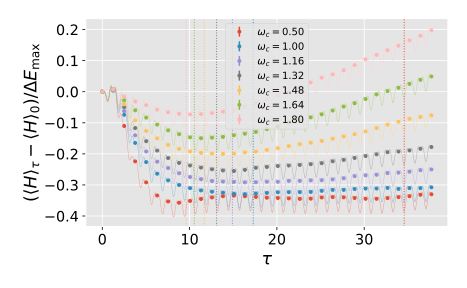
\includegraphics{figs/one_bath_mod/omegas_total}
  \caption{\label{fig:omegas_total} The total energy differences of
    \cref{eq:one_qubit_model_driven} for various cutoffs
    \(ω_{c}\). For details on the parameters see
    \cref{fig:omega_couplings_and_energies}. The dots mark the times
    when the interaction Hamiltonian vanishes.  The dashed lines show the
    position of the where the total energy is minimal. Lower cutoffs
    \(ω_{c}\) lead to more extracted energy. For \(ω_{c}=2.1\) (pink) no
    energy is being extracted at all.}
\end{figure}
It is clear, that a lower cutoff frequency is advantageous as the
minimal total energy is achieved earlier and is of greater
magnitude. Further, we see that a non-trivial amount of energy
\(\sim 35\%\) is being extracted relative to the ergotropy bound
\cref{eq:ergo_mod_model}. This is an important result, as it shows
that the bound \cref{eq:ergo_mod_model} derived in
\cref{sec:ergoonebath} does not only constitute an abstract upper
limit on energy extraction, but can actually be approached.

\begin{figure}[htp]
  \centering
  \includegraphics{figs/one_bath_mod/omega_energies_and_powers}
  \caption{\label{fig:omegas_energies_and_powers} One shot power
    (blue) and maximal extracted energy (orange) as a function of the
    bath memory. The grey vertical line marks one modulation
    period. Longer memories lead to greater energy extractions and
    greater one shot power.}
\end{figure}
\Cref{fig:omegas_energies_and_powers} plots the maximal extracted
energy (orange) and one shot power (blue) as a function of bath memory
time.  The bath memory time is defined here as the time point at which
\(α(τ_{\bath}) = α(0)/10\) which leads to \(τ_{\bath}=3/ω_{c}\) for
the Ohmic BCF. The one shot power is defined as
\begin{equation}
  \label{eq:one_shot_power}
  P_{\max}=\max_{n\in\NN}\frac{\abs{Δ\ev{H}_{n τ_{m}} \cdot Θ(-Δ\ev{H}_{n τ_{m}})}}{n τ_{m}},
\end{equation}
where \(Δ\ev{H}_{τ}= \ev{H}_{τ} - \ev{H}_{0}\) and \(Θ\) is the
Heaviside function.

The plot shows that longer bath memories, lead to both increased
energy extraction and increased one shot power.  The concrete shape of
the curve \cref{fig:omegas_energies_and_powers} is hard to discuss
because of the nontrivial shape and magnitude of the spectral
densities. However, the abrupt transition to zero for short memories
is due to the requirement that power and extracted energy have to be
positive and the stroboscopic time view induced by the requirement
that the interaction energy has to be zero.

It can be concluded that in the cases studied here we can extract a
finite amount of energy from the system as soon as the bath memory is
somewhat longer than the modulation period. This statement depends on
the definition of the memory time \(τ_{\bath}\) and has therefore to
be taken as a rule of thumb.

A peculiar observation has been made for the simulations with very low
cutoff \(ω_{c}\lesssim 1\). \Cref{fig:total_for_steady} shows that we
don not enter a periodic steady state where a constant amount of
energy is being introduced into the system. Rather the total energy
remains constant apart from minor oscillations.
\begin{figure}[htp]
  \centering
  \includegraphics{figs/one_bath_mod/total_for_steady}
  \caption{\label{fig:total_for_steady} The \(ω_{c}=0.5\) simulation
    of \cref{fig:omegas_total} continued for longer times. The total
    energy remains constant apart from minor fluctuations.}
\end{figure}
This feature must be somewhat robust, as it is also visible for
\(ω_{c}=0.96\) in \cref{fig:omegas_total}. Such behaviour is not
forbidden by the results of \cref{sec:therm_results}, but nevertheless
interesting for future study as it corresponds to a situation where
modulate the system indefinitely without having to put in energy.

Another avenue for exploration would be to exploit the findings here
to construct a cyclic thermal machine with high power output. An
interesting question is, whether energy can then be extracted both
during contact with the hot and with the cold bath and whether it is
better to design the cycle stroke based or continuously coupled.

For now, we stick to our model and explore the effect of changing the
modulation frequency \(Δ\) in \cref{sec:speedlim}.

\subsection{Modulation Frequency and Speed Limit}%
\label{sec:speedlim}
Another interesting parameter to tune is the modulation frequency
\(Δ\) or, equivalently, the modulation period \(τ_{p}=2π/Δ\). In
driven systems, there usually appears a ``quantum speed
limit''~\cite{Kurizki2021Dec} that limits the power output of a driven
system at a given coupling strength. An example is the transition from
engine to refrigerator in a continuously coupled two-bath engine in
\cite{Mukherjee2020Jan}. More generally, this issue is connected to
non-adiabatic changes in the Hamiltonian that can generate non-passive
states \cite{Binder2018}.

Intuitively speaking, slower modulation allows more time for the
system-bath interaction that enables energy extraction from the
initially passive bath state in the first place. Fast modulation can
dominate the action of the bath in the interaction term of
\cref{eq:one_qubit_model_driven}, leading to an increase in total
energy.

The continuous power is given by
\begin{equation}
  \label{eq:power_for_onequbit}
  P = \ev{\dot{H}_{\inter}} \sim Δ \sin(Δ) \ev{B σ_{x}^{†} + \hc},
\end{equation}
where \(H_{\inter, m} \equiv \ev{B σ_{x}^{†} + \hc}\) constitutes the
unmodulated interaction Hamiltonian. Increasing the frequency \(Δ\)
will increase the amplitude of \cref{eq:power_for_onequbit}. On the
other hand, if the expectation value of \(H_{\inter, m}\) does not
change much or on a much slower scale than \(τ_{p}\) because of too
fast modulation, the \(Δ\sin(Δ)\) factor will cause the expression to
average out to zero (Zeno-like effect,~\cite{Kurizki2021Dec}).

Stronger coupling will lead to a greater expectation value of
\(H_{\inter, m}\) and generically to more power in the region in
parameter space we are going to explore.

To assess the behaviour with regard to coupling and modulation speed,
we simulated the model for \(ω_{c}=1\) up to the time \(τ=20\) for
various coupling strengths and modulation frequencies. To ease
interpretation, we plotted the resulting one shot powers
\cref{eq:one_shot_power} in a heatmap in \cref{fig:power_heatmap}. The
coupling strength is quantified by the value of the thermal bath
correlation function \(α_{β}\)
\begin{equation}
  \label{eq:finite_bcf_1}
  \begin{aligned}
  α_{β}(τ)&=\frac{1}{π}∫_{0}^{∞} J(ω) \bqty{2\bose(βω) \cos(ω (t-s)) - \iu
        \sin(ω (t-s))} \dd{ω}\\
    &= \frac{1}{π} ∫_{-∞}^{∞} \bqty{\bose(\abs{βω})+Θ(ω)} J(\abs{ω})
  \eu^{-i ω t}\dd{ω},
  \end{aligned}
\end{equation}
at time zero. This choice balances the shifting of the spectral
density for the different values of \(Δ\).

\begin{figure}[htp]
  \centering
  \includegraphics{figs/one_bath_mod/power_heatmap}
  \caption{\label{fig:power_heatmap} Left panel: The one shot power
    \cref{eq:one_shot_power} of the model
    \cref{eq:one_qubit_model_driven} is plotted for various modulation
    frequencies \(Δ\) and coupling strengths. The parameters
    \(ω_{c}=1,λ=0.1, T=5\) were used. Right panel: The same, but
    normalized to the maximum power for each coupling strength
    \(α_{β}(0)\). In both cases \(100\) grid points and Gaussian
    interpolation have been used. The power output generally increases
    with the coupling strength, but the optimal modulation frequency
    becomes more sharply defined (right panel).}
\end{figure}
\begin{figure}[htp]
  \centering
  \includegraphics{figs/one_bath_mod/power_en_heatmap}
  \caption{\label{fig:power_heatmap_tuned} Like
    \cref{fig:power_heatmap_tuned} but as function of maximal
    interaction energy as in \cref{sec:extr_mem}.  The parameters of
    the underlying simulations can be found in
    \cref{tab:plus_mod_en}. A broadly similar behaviour to
    \cref{fig:power_heatmap} can be observed.}
\end{figure}

We find that a larger power output is achieved by stronger
coupling. The dependence on the modulation frequency exhibits more
nuances. If the power output is normalized by its maximum value for
each coupling strength \(α_{β}(0)\) it can be observed that the
optimal power output is achieved at roughly the same modulation
frequency for all coupling strengths. However, with increasing
coupling, the system becomes more sensitive to the modulation
frequency, exhibiting a clear maximum. This constitutes the ``speed
limit'' discussed above. Intuitively speaking, a stronger coupling
increases the time resolution of the interaction, making it more
sensitive to the modulation frequency.

Running the simulations with a peak interaction energy target like in
\cref{sec:extr_mem} gives broadly similar results on the level of
detail available to us, as can be ascertained from
\cref{fig:power_heatmap_tuned}. For the \(Δ=1\) case the optimization
was generally not very effective in the weaker coupling regime as is
quantified in \cref{fig:interaction_tuning_success} on
\cpageref{fig:interaction_tuning_success}. Therefore this region
should be interpreted with care.

The above results have to be taken with a grain of salt however. The
grid resolution of 10 by 10 does not allow us to perceive a possible
small shift in the optimal modulation frequency. Also, the range of
interaction strengths is rather limited.

\begin{figure}[htp]
  \centering
  \includegraphics{figs/one_bath_mod/interaction_nontuned}
  \caption{\label{fig:interaction_nontuned} Left panel: Similar to
    \cref{fig:power_heatmap} but showing the maximal absolute
    interaction energies. Right panel: A log-log-plot of the maximal
    interaction energy over the coupling strength. The dashed grey
    line is a linear reference curve.}
\end{figure}

The maximal absolute values of the interaction energy are shown in
\cref{fig:interaction_nontuned} for the non-optimized case of
\cref{fig:power_heatmap}. Generally, the energy increases with
increasing coupling strength as is sensible. The dependence on the
coupling strength is linear for modulations with \(Δ\geq 5\) but
deviates for slower modulation. This may be due to the fact, that
fewer modulation periods can be completed in the given time frame.

The interaction energy also increases for faster modulation,
especially at greater coupling strengths. Comparing
\cref{fig:interaction_nontuned} with \cref{fig:power_heatmap} we see
that the top right region where the interaction energy is strongest
somewhat coincides with a decrease in power. In this region, the
dependence of the interaction energy on the modulation frequency is
also most pronounced.  The \(Δ=1\) case is an outlier as we already
noted above and should therefore be interpreted with care. It is
likely that not enough cycles have been simulated to judge this case
accurately.

Summarizing, we found that the one shot power output for the model
\cref{eq:one_qubit_model_driven} has a complex dependence on the
coupling strength and the modulation frequency. Especially for strong
coupling the modulation frequency has to be chosen carefully if
optimal energy extraction is to be achieved.

The resonance criterion that motivated the shift of the spectral
density of the bath has not been substantiated as of now. Therefore we
will briefly discuss its systematics in \cref{sec:modcoup_reso}.

\subsection{Resonance Behaviour of the One Shot Power}
\label{sec:modcoup_reso}
Finally, after having introduced the shift of the spectral density on
a rather vague basis, we would like to give a short demonstration of
its validity.

To this end we choose the zero temperature spectral densities with
their peaks slightly shifted away from \(1+Δ\) to \(1+Δ+δ\) and
normalized so that their peak height is fixed.
\begin{figure}[htb]
  \centering
  \includegraphics{figs/one_bath_mod/modulation_tuning}
  \caption{\label{fig:modulation_tuning} Left panel: The one shot
    power \cref{eq:one_shot_power} for multiple values of the detuning
    \(δ\) and three peak heights of the zero temperature spectral
    density. Right panel: The spectral densities for the peak height
    \(J_{\mathrm{peak}} = 0.5\). The dotted lines are the positive
    frequency parts of the effective finite temperature spectral
    density \(\bqty{\bose(\abs{βω})+Θ(ω)} J(\abs{ω})\) (see also
    \cref{eq:finite_bcf_1}). The detailed model and simulation
    parameters can be found in \cref{tab:plus_tune}.}
\end{figure}

\Cref{fig:modulation_tuning} shows the one shot power
\cref{eq:one_shot_power} as a function of the detuning for different
coupling strengths as quantified by the spectral density peak
height. In all cases, the one shot power exhibits a clear maximum
which demonstrates the resonance effect.

For the strongest coupling case (green) we find in
\cref{fig:modulation_tuning} that the optimal peak position has moved
slightly to the right.  Note also that even though the finite
temperature spectral density decreases in magnitude for positive
shifts the power increases, so that the observed behaviour is not
explained by finite temperature. Also, the penalty for being off
resonant in the negative \(δ\) direction is much more severe than in
the weaker coupling cases (orange, blue).

An explanation may be, that higher harmonics like \(1+ 2 Δ\) become
important for stronger coupling. Shifting the spectral density
slightly to higher frequencies then optimizes the resonance with those
harmonics. In general, we find that the behavior of the model also
depends on the shape of the spectral density and not only on its value
at the peak. This is consistent with \cref{sec:energy-transf-char}
and~\cite{Xu2022Mar}, where a similar behavior was observed.

As a final application of the HOPS formalism to thermodynamical
systems, we demonstrate a thermodynamic cycle that produces finite
power at finite efficiency in \cref{sec:otto}.

\section{Quantum Otto Cycle}%
\label{sec:otto}
To exploit the whole range of capabilities of the NMQSD and HOPS we
now turn to a model with multiple baths at different
temperatures. This also provides us with an opportunity to demonstrate
the usefulness and validity of the considerations of
\cref{sec:operational_thermo}, namely the bound on extractable energy
per cycle and efficiency, as well as the cost measure introduced
there.

A standard thermodynamic cycle that is a popular model in the
literature\footnote{see
  \cite{Wiedmann2021Jun,Karimi2016Nov,Binder2018}} is a quantum heat
engine inspired by the Otto cycle. Similar to expansion and
compression of an ideal gas, we modulate the level spacing of our
qubit working medium. This model serves as a good demonstration of
HOPS' capabilities when it comes to the modulation of the coupling and
the system in arbitrary ways.

Here, we consider a spin boson model much like the one in
\cref{sec:singlemod} but with two baths
\begin{equation}
  \label{eq:otto_model}
  H = \frac{1+f(t)}{2} (σ_z+1) +
  ∑_{i\in\{h, c\}}\bqty{h_{i}(t) σ_{x} ∑_λ\frac{1}{2}\qty(g_{λ,i} a_{λ,i} + g_{λ,i}^\ast
    a_{λ,i}^†) + ∑_λ ω_{λ,i} a_{λ,i}^\dag a_{λ,i}.}
\end{equation}
The modulation functions \(f\) and \(h_{i}\) are periodic and
constructed out of smoothstep\footnote{see \cref{sec:smoothstep}}
functions similar to \cite{Wiedmann2021Jun}. The subscripts \(h,c\)
stand for hot and cold respectively and refer to the bath
temperatures.  Rather than giving the precise formulas, we instead
plot the modulation functions over one period in \cref{fig:ottomod}.
\begin{figure}[htp]
  \centering
  \includegraphics{figs/otto/modulation}
  \includegraphics{figs/otto/spectral_densities}
  \caption{\label{fig:ottomod} Left panel: One period of the
    modulation functions in \cref{eq:otto_model}. Right panel: The
    finite temperature effective spectral densities
    \(\bqty{\bose(\abs{βω})+Θ(ω)} J(\abs{ω})\) of the hot and cold
    baths. The dots mark the level spacing of the system Hamiltonian
    in the cold and hot phase.}
\end{figure}

The protocol can be decomposed into strokes as follows. First, the
energy gap is widened from one to two (widening stroke) which requires
the expenditure of energy. After this, the system is coupled to a hot
bath to ``charge'' for some time and decoupled before the energy gap
is being compressed from two to one again (narrowing stroke) which
extracts energy. Finally, the qubit is being ``reset'' by shedding
energy into a low temperature bath.

The effective finite temperature spectral densities with \(ω_{c}=1\)
have been shifted so that their value is maximal for a given
temperature at the frequency of the system in its compressed (cold) or
expanded (hot) state. Their magnitudes have been chosen so that their
values at these points are the same as can be seen in
\cref{fig:ottomod}.

We initialize the system in the \(H_{\sys}\ket{0}=0\) state. The
temperatures of the baths were set to \(T_{c}=1\) and \(T_{h}=20\) so
that both temperatures are finite but convergence is achieved with a
reasonable number of trajectories. The interaction strength has been
chosen to be relatively weak for the same reason and also to be closer
to the known weak coupling realm.

In comparison to the system timescale, the modulation cycle is rather
slow. On the other hand, the time scales on which \(f\) and \(h_{i}\)
change are not adiabatic.

\begin{figure}[htp]
  \centering
  \includegraphics{figs/otto/power}
  \caption{\label{fig:ottopower} The power due to the system and the
    bath modulation of the Otto cycle model \cref{eq:otto_model}. The
    total power is
    \(\ev{\dot{H}} = \ev{\dot{H}_{\sys}} +
    \ev{\dot{H}_{\inter}}\). The interaction power is not negligible
    and in this case generally detrimental to the performance.}
\end{figure}
\Cref{fig:ottopower} shows the power due to the modulation of the
system (orange) and the interaction (blue) Hamiltonians, where the
major contribution to the total power is the system. The narrowing
stroke produces negative (usable) power and the widening produces
positive power that has to be supplied externally. More importantly
however, we find that also the modulation of the interaction, i.e. the
coupling and decoupling, figures into the total power and reduces the
energy output. In a weak coupling scheme, this contribution can be
neglected. Not so however in the generic case presented here. A
similar result was found in~\cite{Wiedmann2021Jun}.

The mean power output of this cycle is
\(\bar{P}=0.002468\pm 0.000021\) with an efficiency, as defined in
\cref{eq:efficiency_definition}, of \(η=29\%\). Without special tuning
except for the shifts in the spectral densities we achieved finite
power and efficiency.

Neglecting the energy change due to the coupling modulation we find
instead \(\bar{P}=0.004337\pm 0.000018\) and \(η=52\%\).  This
efficiency is, likely coincidentally, close to the efficiency given in
\cite{Geva1992Feb} for the quantum Otto cycle under quasistatic
conditions. In any case we are quite far from the Carnot efficiency
for the given temperatures \(η_{c}=95\%\).

\begin{figure}[htp]
  \centering
  \includegraphics{figs/otto/energy_strobe}
  \caption{\label{fig:ottoenergy} The system \(\ev{H_{\sys}}\), bath
    \(\ev{H_{\bath^{h,c}}}\) and interaction energy
    \(\ev{H_{\inter^{h,c}}}\) as well as the total energy change
    \(\ev{H}-\ev{H}_{τ=0}\) of the model \cref{eq:otto_model}. The
    dots mark the times where one cycle is completed.}
\end{figure}
In \cref{fig:ottoenergy} we show the full energy dynamics of the
simulation. The interaction energy for the coupling to the hot bath
(violet line) is almost negligible, while the interaction with the
cold bath (green line) is stronger. However, the system energy change
in the hot and cold thermalization stroke (blue line) is of similar
magnitude.  A periodic steady state is reached after roughly two
cycles. In this steady state, the system and interaction related
quantities are constant in the stroboscopic view (the dots in
\cref{fig:ottoenergy}), while the total energy and the bath energies
exhibit a constant change over each cycle period. The assumptions of
\cref{sec:operational_thermo} are being met precisely.

We do not see oscillations in the bath energy which would
indicate the more complicated energy transfer behaviour we found in
\cref{sec:one_bath_cutoff}, signifying that we are working in a rather
``tame'' regime as intended.

The Gibbs like inequality \cref{eq:secondlaw_cyclic} derived in
\cref{sec:operational_thermo} can also be verified in this case.
We find
\begin{equation}
  \label{eq:secondlaw_otto_actual}
  ∑_iβ_i ΔE_{\bath^i}^\cyc = 0.1096\pm 0.0008 ≥ 0,
\end{equation}
which does satisfy the inequality to over 100 standard
deviations. Minimizing this dimensionless quantity maximizes the
efficiency.

With this cycle, little coherence is generated\footnote{see
  \cref{eq:otto_coherences} on \cpageref{eq:otto_coherences}} leading
so called ``frictionless'' dynamics. See also \cref{eq:otto_bloch} for
a plot of the trajectory of the system density matrix in the bloch
sphere.

Because it requires little additional effort, we can briefly explore a
continuously coupled version off this model, where the coupling
modulation is switched off, and we thus have \(h_{h,c}(τ)=1\). We find
in \cref{fig:ottoenergy_cont} that work extraction is still possible,
albeit at a much lower power output \(\bar{P}=0.001670\pm 0.000029\)
and efficiency \(η=5\%\).
\begin{figure}[htp]
  \centering
  \includegraphics{figs/otto/energy_strobe_continuous}
  \caption{\label{fig:ottoenergy_cont} The system, bath and
    interaction energies as well as the total energies of the model
    \cref{eq:otto_model} for continuously coupled baths. The dots mark
    the times where one cycle is completed. We can observe positive
    energy extraction albeit at a much reduced power
    \(\bar{P}=0.001670\pm 0.000029\) and efficiency \(η=5\%\) compared
    to the modulated case in \cref{fig:ottoenergy}.}
\end{figure}

The finite energy extraction is due to the baths being alternately
resonant and off-resonant. Increasing the amplitude of the system
modulation and consequently the gap between the peaks of the spectral
densities should improve the performance.

The lost efficiency is due to energy flowing ``through'' the system
unused, a behaviour which is promoted by the continuous coupling and
reflected in the much higher entropy production
\(∑_iβ_i ΔE_{\bath^i}^\cyc = 0.6198\pm 0.0021\).

Nevertheless, if the cycle was very fast, the effect of the
(un)coupling of the baths could be so detrimental that the
continuously coupled version of the cycle is superior. See also the
remarks in \cref{cha:concl-ideas-future} about \cite{Uzdin2015Sep}.


% \section{Anti Zeno Engine}
% \label{sec:antizeno}
% \begin{itemize}
% \item mention concept
% \item results not reliable in time for thesis
% \item interesting because: non-Markovian QUANTUM advantage. a bit
%   sensational ;P
% \end{itemize}


% \begin{itemize}
% \item ... list all those nice papers ...
% \item the third law
% \item look more deeply into the peculiarities in \cref{sec:oneosccomp}
% \item verify speculation of energy flow vs non-markvianity: flow
%   between two baths though a system
% \item three level system -> paper
% \item driven spin boson -> paper \cite{Magazzu2018Apr}
% \item flows crossing in one point: robust featureu
% \item linear regeime of steady state energies -> universal, how far
%   does it extend
% \item more detailed parameter scans, universality between different models?
% \item state changes -> is energy difference = heat + work path
%   independent (maybe try different protocols and turn off interaction
%   at for beginning and end in an adiabatic way...)
% \item compare with results from master equation in \cref{sec:prec_sim}
% \item steady state methods, better convergence for long-time
%   simulations
% \item coupling to single bath: although breach of second law forbidden
%   -> cyclical energy transfer for very long bath correlation times
% \item filter mode: \cref{sec:shift_sp}
% \item otto cycle: sensitivity to timing stronger with stronger coupling?
% \end{itemize}

\chapter{Conclusion and Outlook}
\label{cha:concl-ideas-future}

In this work, we set out to find a way of accessing bath related
observables, such as the expected bath energy change and the
interaction energy expectation value, using the
NMQSD\footnote{Non-Markovian Quantum State
  Diffusion}/HOPS\footnote{Hierarchy of Pure States} framework which
we introduced in \cref{chap:intro}.  This endeavor was indeed
successful as was laid out in \cref{chap:flow}.

In \cref{chap:flow} we presented a solution to a well known model for
quantum Brownian motion. Using this solution, we were able to derive
expressions for the bath energy change \(∂_{t}\ev{H_{\bath}}\).

This enabled us to verify the results of \cref{chap:flow} in
\cref{chap:numres} by solving the same model numerically using
HOPS. Excellent agreement was found in
\cref{sec:hopsvsanalyt}.

Turning to the spin-boson model in \cref{sec:prec_sim}, we used energy
conservation to verify again, that we can consistently and efficiently
compute bath related observables with HOPS. In the cases where the
consistency condition was not met, we nevertheless found that
qualitatively correct results had been reached. The direct calculation
of the interaction energy by the use of \cref{sec:intener} gives
results that are more precise than the ones obtained through energy
conservation.

We continued to explore the energy transfer behavior of the zero
temperature spin-boson model and found that energy transfer
performance for strong coupling has a complicated dependence on the
spectral density of the bath. Energy transfer performance can be
optimized longer bath memories and resonant baths when the interaction
is turned off at the right time.

The short time dynamics of the bath energy change can be explained by
neglecting the system Hamiltonian, which we verified for the
spin-boson model. It was also found, that this short time behaviour is
already present on the trajectory level so that there are no
stochastic fluctuations for short times. During this initial period,
the auxiliary states of the HOPS are being populated.

In \cref{sec:singlemod} we turned to issues of quantum
thermodynamics. We reviewed some general analytical results that
bounded energy extraction from open systems in
\cref{sec:basic_thermo}, both for the single-bath and the multi-bath
case. We then turned to some more challenging applications of the HOPS
method. First, a driven spin-boson model was considered. We found that
a not insignificant fraction of the theoretical maximum of energy can
be extracted by modulating the coupling and providing a bath with long
memory time. We also demonstrated quantum friction, a quantum speed
limit and a bath resonance phenomenon.

Finally, we treated a model with multiple baths in \cref{sec:otto} and
non-harmonic smooth modulation. A cyclic modulation protocol was
implemented upon a two level system coupled to two baths in a
spin-boson like fashion. We achieved finite power with finite
efficiency and verified a Gibbs-like inequality
\cref{sec:operational_thermo}. When disabling the coupling modulation,
the power and efficiency were much reduced.

A worthwhile task for future work would be to verify the results
summarized in \refcite{Binder2018} for the Otto cycle. Especially the
optimization for optimal power which leads to the
Novikov–Curzon–Ahlborn efficiency \(η_{ca}=1-\sqrt{T_{c}/T_{h}}\) is
interesting in the case of stronger coupling.

Another cycle to study would be a Carnot-type cycle, where the
modulation of the system and the thermalization with the bath occur at
the same time. Interpolating between Otto and Carnot, as well as
studying the effect of overlapping and shifting strokes is a
fascinating avenue for future exploration.

Also, more interesting working media, such as a three level system are
of interest. In \refcite{Uzdin2015Sep} it is shown, that in certain
regimes quantum coherence can lead to superior power output. In the
same regime different types heat engines are equivalent. Both these
effects have been observed experimentally in \refcite{Klatzow2019Mar}. It
would be interesting to see if the slight deviations from theory in
\cite{Klatzow2019Mar} could be explained using HOPS.

The so called Anti-Zeno Effect occurring in systems under fast
modulation has recently received some attention
\cite{Mukherjee2020Jan,Xu2022Mar}. An advantage is claimed to exist,
due to the broadening of the resonance criterion which we have
observed in
\cref{sec:one_bath_cutoff,sec:modcoup_reso,sec:otto}. Being a
consequence of the energy time uncertainty it is being argued, that
the origin of this advantage is truly quantum. The tools for the
exploitation of this effect and its verification are provided in this
work. However, a strong coupling analysis has already been performed
using HEOM in \refcite{Xu2022Mar}.

In \refcite{Santos2021Jun} a cycle is proposed that first creates states
of finite ergotropy by letting energy flow through the working medium
and then extracting this ergotropy in a separate stroke. This work
could be verified and expanded to the non-Markovian regime.

A useful improvement of the method would be the ability to snapshot
the total state of system and bath and then propagate this state with
different modulation protocols. Also, exploring the thermofield method
for finite temperature to avoid the slow convergence of the flow may
be worthwhile. However, at least for coupling that is not hermitian,
this would only trade computational effort for memory, as the number
of hierarchy states would increase.

Finally, in the spirit of~\cite{Esposito2015Dec} one could employ the
HOPS to verify whether a given definition of internal energy that
includes the interaction energy is path independent.


\begin{appendices}
\chapter{Some Notes on HOPS}
\label{chap:hops_notes}
\section{Normalized HOPS}%
\label{sec:norm}

We introduce full HOPS vector \(Ψ = \qty(ψ, φ)\) which can be
decomposed into the zeroth hierarchy order state \(ψ\) and the
non-zero order states \(φ\).

The HOPS equations can then be written in an abstract manner as
\begin{equation}
  \label{eq:HOPS}
  \begin{aligned}
    \dot{ψ} &= F(ψ, φ), & \dot{φ} &= G(ψ, φ),
  \end{aligned}
\end{equation}
where \(c\cdot F(ψ, φ) = F(c\cdot ψ, c\cdot φ)\) and
\(c\cdot G(ψ, φ) = G(c\cdot ψ, c\cdot φ)\) for \(c\in\CC\)


The goal is to transform \(ψ \rightarrow \tilde{ψ}\) so that
\begin{equation}
  \label{eq:goal}
  \norm{\tilde{ψ}} = 1
\end{equation}
in a numerically stable manner.

Introducing the definitions \(\tilde{ψ} = \eu^{f(t)}ψ\) and
\(\tilde{φ} = \eu^{f(t)}φ\) with an
arbitrary\(f\colon \RR \rightarrow \CC\) we can begin to calculate
\begin{equation}
  \label{eq:normdgl}
  ∂_t\norm{\tilde{ψ}}^2 = \tilde{ψ}^† \qty(\dot{f}\tilde{ψ} +
  F(\tilde{ψ}, \tilde{φ})) + \cc = \dot{f} \abs{\tilde{ψ}}^2 +
  \tilde{ψ}^†F(\tilde{ψ}, \tilde{φ}) + \cc.
\end{equation}

We would now like to obtain \(∂_t\norm{\tilde{ψ}}^2 = 0\) as well as
\(\dot{f} > 0\) for \(\norm{\tilde{ψ}} < 1\), \(\dot{f} < 0\) for
\(\norm{\tilde{ψ}} > 1\) and \(\dot{f} = 0\) for
\(\norm{\tilde{ψ}}=1\), so that \(\norm{\tilde{ψ}} = 1\) becomes a
stable fix-point.

Observing \cref{eq:normdgl}, we conclude that our goals can be
achieved by demanding
\begin{equation}
  \label{eq:fdgl}
  \dot{f} = \frac{\tilde{ψ}^†F(\tilde{ψ},
    \tilde{φ})}{\norm{\tilde{ψ}}^2} + g\qty(\norm{ψ}^2)
\end{equation}
with \(g(0)=0\).

The first summand on its own would lead to norm conservation, \(∂_t\norm{\tilde{ψ}}^2 =
0\). The latter of our goals may be achieved by
choosing \(g(x) = \qty(1-x)\).

These choices lead to an altered HOPS equation
\begin{equation}
  \label{eq:normedhops}
  \dot{\tilde{Ψ}} = \qty[\frac{\tilde{ψ}^†F(\tilde{ψ},
    \tilde{φ})}{\norm{\tilde{ψ}}^2}+\qty(1-\norm{\tilde{ψ}}^2)]\mqty(\tilde{ψ}\\
  \tilde{φ}) + \mqty(F(\tilde{ψ},\tilde{φ}) \\ G(\tilde{ψ},\tilde{φ})).
\end{equation}

\section{Multiple Baths}
\label{sec:hops_multibath}

We generalize the NMQSD and HOPS to \(N\) baths for Hamiltonians of
the form~\cref{eq:multimodel}.


\subsection{NMQSD}
\label{sec:nmqsd}

Following the usual derivation of the NMQSD \cite{Diosi1998Mar}, we
switch to an interaction picture with respect to the \(H_\bath\)
leading to
\begin{equation}
  \label{eq:multimodelint}
  H(t) = H_\sys + ∑_{n=1}^N \qty[L_n^†B_n(t) + \hc],
\end{equation}
with \(B_n=∑_{λ} g_λ\nth a_λ\nth\eu^{-\iu ω_λ\nth t}\).

We will discuss the zero temperature case. The finite temperature
methods generalize straight forwardly to multiple baths.  Projecting
on a Bargmann (unnormalized) coherent state basis
\(\qty{\ket{\vb{z}^{(1)},\vb{z}^{(2)},\ldots}=
  \ket{\underline{\vb{z}}}}\) of the baths
\begin{equation}
  \label{eq:projected}
  \ket{ψ(t)} = ∫∏_{n=1}^N{\qty(\frac{\dd{\vb{z}\nth}}{π^{N_n}}\eu^{-\abs{\vb{z}}^2})}\ket{ψ(t,\underline{\vb{z}}^\ast)}\ket{\underline{\vb{z}}},
\end{equation}
where \(N_n\) are the number of oscillators in each bath.


We define
\begin{equation}
  \label{eq:processes}
  η^\ast_n(t) = {\qty(\vb{η}^\ast_t)}_n= -\iu ∑_λg_λ^{(n),\ast} z_λ^{(n),\ast}\eu^{\iu ω_λ\nth t}
\end{equation}
and using
\(\pdv{z_λ^{(n),\ast}}=∫\dd{s}\pdv{η^\ast_n(s)}{z_λ^{(n),\ast}}\fdv{η^\ast_n(s)}\)
we arrive at
\begin{equation}
  \label{eq:multinmqsd}
  ∂_tψ_t(\vb{η}^\ast_t) = -\iu H ψ_t(\vb{η}^\ast_t) +
  \vb{L}\cdot\vb{η}^\ast_tψ_t(\vb{η}^\ast_t) - ∑_{n=1}^N L_n^†∫_0^t\dd{s}α_n(t-s)\fdv{ψ_t(\vb{η}^\ast_t)}{η^\ast_n(s)},
\end{equation}
where \(α_n(t-s)= {\qty(\vb{α}(t-s))}_n=∑_λ\abs{g_λ\nth}^2\eu^{-\iu ω_λ\nth(t-s)}\) are the
zero temperature bath correlation functions. The equation
\cref{eq:multinmqsd} becomes the NMQSD by reinterpreting the
\(\vb{z}\nth\) as normal distributed complex random variables by
virtue of monte-carlo integration of \cref{eq:projected}. The
\(η^\ast_n(t)\) become homogeneous gaussian stochastic processes
defined through
\begin{equation}
  \label{eq:processescorr}
  \begin{aligned}
      \mathcal{M}(η^\ast_n(t)) &=0, & \mathcal{M}(η_n(t)η_m(s)) &= 0,
      & \mathcal{M}(η_n(t)η_m(s)^\ast) &= δ_{nm}α_n(t-s).
  \end{aligned}
\end{equation}

\subsection{Nonlinear NMQSD}
\label{sec:nonlin}

For the derivation of the lonlinear theory, the characteristic
trajectories of the partial differential equation of motion of
the Husimi-function
\begin{equation}
  \label{eq:husimi}
  Q_t(\underline{\vb{z}}, \underline{\vb{z}}^\ast) =
  \frac{\eu^{-\abs{{\underline{\vb{z}}}}^2}}{π^{∑_n N_n}}
  \braket{ψ(t, {\underline{\vb{z}}})}{ψ(t, {\underline{\vb{z}}}^\ast)}
\end{equation}
have to be determined.

Using \(∂_{\underline{\vb{z}}}\ket{ψ(t, {\underline{\vb{z}}}^\ast)} =
0\) and \(∂_{\underline{\vb{z}}^\ast}\bra{ψ(t, {\underline{\vb{z}}})} =
0\) because \(\ket{ψ(t, {\underline{\vb{z}}}^\ast)}\) is holomorphic
we derive
\begin{equation}
  \label{eq:husimimotion}
  ∂_tQ_t(\underline{\vb{z}}, \underline{\vb{z}}^\ast) = -i
  ∑_{n=1}^N\qty[∂_{z_λ^{(n), \ast}}\eu^{-\iu ω_λ\nth
    t}\ev{L^†_n}_tQ_t(\underline{\vb{z}}, \underline{\vb{z}}^\ast) - \cc],
\end{equation}
where \(\ev{L^†_n}_t = \mel{ψ(t, {\underline{\vb{z}}})}{L^†_n}{ψ(t,
  {\underline{\vb{z}}}^\ast)} / \braket{ψ(t, {\underline{\vb{z}}})}{ψ(t, {\underline{\vb{z}}}^\ast)}\).

The characteristics of \cref{eq:husimimotion} obey the equations of
motion
\begin{equation}
  \label{eq:characteristics}
  \dot{z}^{(n),\ast}_λ = \iu g_λ\nth \eu^{-\iu ω_λ\nth t} \ev{L^†_n}_t
\end{equation}
for the stochastic state labels.

The microscopic dynamics can in-turn be gathered into a shift of the
stochastic processes
\begin{equation}
  \label{eq:procshift}
  \tilde{η}_n^\ast(t) = η_n^\ast(t) + ∫_0^t\dd{s}α_n^\ast(t-s)\ev{L^†_n}_s
\end{equation}
and we obtain the nonlinear NMQSD equation
\begin{multline}
  \label{eq:multinmqsdnonlin}
  ∂_tψ_t(\tilde{\vb{η}}^\ast_t) = -\iu H ψ_t(\tilde{\vb{η}}^\ast_t) +
  \vb{L}\cdot\tilde{\vb{η}}^\ast_tψ_t(\tilde{\vb{η}}^\ast_t) \\-
  ∑_{n=1}^N
  \qty(L_n^†-\ev{L^†_n}_t)∫_0^t\dd{s}α_n(t-s)\eval{\fdv{ψ_t(\tilde{\vb{η}}^\ast_t)}{η^\ast_n(s)}}_{\vb{η}^\ast(s)
  = \vb{η}(\underline{\vb{z}}^\ast(t), s)}.
\end{multline}

The notation
\({\vb{η}^\ast(s) = \vb{η}(\underline{\vb{z}}^\ast(t), s)}\) means
that we replace the microscopic \(z_λ^{(n),\ast}\) in
\cref{eq:processes} with the shifted ones obeying
\cref{eq:characteristics} and evaluate the resulting function at \(s\).
This awkward construction can be remedied by the convolutionless
formulation. It plays no great role in the HOPS formalism.

\subsection{Multi Bath HOPS in Fock-Space Formulation}
\label{sec:multihops}

Following the usual derivation~\cite{RichardDiss} (but with a
different unitless normalization) and using an exponential expansion of the
BCFs \(α_n(τ)=∑_{\mu}^{M_n}=G_μ\nth\eu^{-W_μ\nth τ}\), we define
\begin{equation}
  \label{eq:dops}
  D_μ\nth(t) \equiv ∫_0^t\dd{s}G_μ\nth\eu^{-W_μ\nth (t-s)}\fdv{η^\ast_n(s)}
\end{equation}
and
\begin{equation}
  \label{eq:dops_full}
  D^{\underline{\vb{k}}} \equiv
  ∏_{n=1}^N∏_{μ=1}^{M_n}
  {\sqrt{\frac{\underline{\vb{k}}_{n,μ}!}{\qty(G\nth_μ)^{\underline{\vb{k}}_{n,μ}}}}
  \frac{1}{\iu^{\underline{\vb{k}}_{n,μ}}}}\qty(D_μ\nth)^{\underline{\vb{k}}_{n,μ}},
\end{equation}
as well as
\begin{equation}
  \label{eq:hierdef}
  ψ^{\underline{\vb{k}}} \equiv D^{\underline{\vb{k}}}ψ.
\end{equation}

Using
\begin{equation}
  \label{eq:commrelation}
  [D^\kmat(t),η_n^\ast(t)] =  \iu∑_{μ=1}^{M_n}
  \sqrt{\kmat_{n,μ}G\nth_μ} D^{\kmat -
    \mat{e}_{n,μ}}
\end{equation}
where \({\qty(\mat{e}_{n,μ})}_{ij}=δ_{ni}δ_{μj}\) we find after some algebra
\begin{multline}
  \label{eq:multihops}
  \dot{ψ}^\kmat = \qty[-\iu H_\sys + \vb{L}\cdot\vb{η}^\ast -
  ∑_{n=1}^N∑_{μ=1}^{M_n}\kmat_{n,μ}W\nth_μ]ψ^\kmat \\+
  \iu ∑_{n=1}^N∑_{μ=1}^{M_n}\sqrt{G\nth_μ}\qty[\sqrt{\kmat_{n,μ}}  L_nψ^{\kmat -
    \mat{e}_{n,μ}} + \sqrt{\qty(\kmat_{n,μ} + 1)}  L^†_nψ^{\kmat +
    \mat{e}_{n,μ}} ].
\end{multline}

The HOPS equations \cref{eq:multihops} can also be rewritten in an
especially appealing form \cite{Gao2021Sep} if we embed the hierarchy
states into a larger Hilbert space using
\begin{equation}
  \label{eq:fockpsi}
  \ket{Ψ} = \sum_\kmat\ket{\psi^\kmat}\otimes \ket{\kmat}
\end{equation}
where
\(\ket{\kmat}=\bigotimes_{n=1}^N\bigotimes_{μ=1}^{N_n}\ket{\kmat_{n,μ}}\)
are bosonic Fock-states.

Now \cref{eq:multihops} becomes
\begin{equation}
  \label{eq:fockhops}
  \begin{aligned}
    ∂_t\ket{Ψ} &= \qty[
                 \begin{aligned}
                 -\iu H_\sys + \vb{L}\cdot\vb{η}^\ast &-
                               ∑_{n=1}^N∑_{μ=1}^{M_n}b_{n,μ}^\dag b_{n,μ} W\nth_μ \\
                   &\qquad+
                 \iu ∑_{n=1}^N∑_{μ=1}^{M_n} \sqrt{G_{n,μ}} \qty(b^†_{n,μ}L_n +
                 b_{n,μ}L^†_n)
                 \end{aligned}
                 ] \ket{Ψ}\\
               &= \tilde{H}\ket{Ψ}
  \end{aligned}
\end{equation}

\section{Estimating the Norms of the Auxiliary States}
\label{sec:normest}

It is possible to find an (semi-rigorous) upper bound to the norms of
the auxiliary states. We will limit ourselves to one bath. The
generalization to multiple baths is straight forward.

Using \cref{eq:fockhops}, we can calculate
\begin{equation}
  \label{eq:normdiff}
  \begin{aligned}
    \iu ∂_t \norm{ψ^{\vb{k}}}^2
    &= \bra{Ψ}\ket{k}\bra{k}\tilde{H}\ket{Ψ} - \cc\\
    &= \qty(ψ^{\vb{k}})^†\bra{k}
      \qty[-\iu L η^\ast -\iu ∑_{μ=1}^{M}b_{μ}^\dag b_{μ} W_μ
      +∑_{μ=1}^{M} \sqrt{G_{μ}} \qty(b^†_{μ}L +
      b_μ L^†)]\ket{Ψ}- \cc\\
    &= \Bigg[-\iu \qty(ψ^{\vb{k}})^†L η^\ast ψ^{\vb{k}}
        -\iu ∑_{μ=1}^{M}k_μ W_μ \norm{ψ^{\vb{k}}}^2\\
        &\phantom{=}\quad -∑_{μ=1}^{M}\qty[\qty(ψ^{\vb{k}})^†\sqrt{G_{μ}k_μ}Lψ^{\vb{k}-\vb{e}_μ} +
        \qty(ψ^{\vb{k}})^†\sqrt{G_{μ}(k_μ+1)}Lψ^{\vb{k}+\vb{e}_μ} ]\Bigg]  - \cc.
  \end{aligned}
\end{equation}

We can now further treat the this expression to find the steady state
norms of the states.

Assuming generically that the term containing the stochastic process
\(η\) vanishes in the time average (as is the case for the steady
state) we will drop it in the following.

Terms of the form \(\Im(ψ^† O φ)\) may be estimated as follows
\begin{equation}
  \label{eq:genericest}
  \abs{\Im(ψ^† O φ)} \leq \norm{ψ} \norm{O φ} \leq \norm{ψ}\norm{O}\norm{φ},
\end{equation}
where the norm on the operator is the standard linear operator norm
\(\norm{O} = \max_{x\in \mathcal{H}}\frac{\ev{O}{x}}{\braket{x}}\).

We now endeavor to find from \cref{eq:normdiff} an estimate of the
steady state norm of \(ψ^{\vb{k}}\). To this end we assume that the
coupling to higher hierarchy states generically lowers the norm and is
therefore neglected. Using \cref{eq:genericest} we can estimate the
influence of the coupling to lower states, choosing the sign
so that the contribution to the norm is positive.

With this we obtain
\begin{equation}
  \label{eq:finalest}
  ∂_t \norm{ψ^{\vb{k}}}^2 = 0 = -∑_{μ=1}^{M}k_μ \Re[W_μ]
  \norm{ψ^{\vb{k}}}^2 +
  ∑_{μ=1}^{M}\abs{\sqrt{G_{μ}k_μ}}\norm{ψ^{\vb{k}}}\norm{ψ^{\vb{k}-\vb{e}_μ}}\norm{L}
\end{equation}
and therefore
\begin{equation}
  \label{eq:steadynorm}
  \norm{ψ^{\vb{k}}} =
  \frac{∑_{μ=1}^{M}\abs{\sqrt{G_{μ}k_μ}}\norm{ψ^{\vb{k}-\vb{e}_μ}}\norm{L}}{∑_{μ=1}^{M}k_μ \Re[W_μ]}.
\end{equation}


For the nonlinear method, the stochastic process obtains a shift whose
magnitude can be estimated as follows
\begin{equation}
  \label{eq:shiftestimate}
  \abs{η_{\mathrm{sh}}} \leq \norm{L} ∫_0^∞\dd{s}\abs{α^\ast(t-s)} \leq
  \norm{L} \sum_{μ=1}^M \frac{\abs{G_μ}}{\Re[W_μ]}.
\end{equation}
It is unclear how this shift should be treated. Simply adding it to
the denominator of~\cref{eq:steadynorm} lead to a breakdown of the
bound for numerical testing.  A better estimate should account for
this and also for the coupling to the lower orders foregoing the
recursive nature of the estimate.

The relation \cref{eq:steadynorm} is recursive
and break off at \(ψ^0\), the norm of which can be assumed to be unity
in the nonlinear method.

These ideas remain to be verified. Especially the assumptions should
be checked. For time dependent coupling, one may maximize the estimate
over all \(L(t)\).

As an illustration the validity of the bound for one specific model
see \cref{fig:normest_ω,fig:normest_δ}.
\begin{figure}[t]
  \centering
  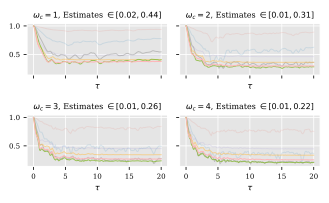
\includegraphics{figs/one_bath_syst/norm_estimate_omega}
  \caption{\label{fig:normest_ω} The maximum norm (for each time
    point) of the first hierarchy states for \(500\) trajectories
    subtracted from norm estimate and normalized by the norm estimate
    for a qubit coupled to single zero temperature ohmic baths
    \cref{eq:one_qubit_model} with varying \(ω_c\). The titles include
    the range of the norm estimates. For higher cutoff frequencies the
    BCF vanishes faster and the norm of the hierarchy states
    decreases. The opacity of the lines is proportional to their
    corresponding \(\abs{G_μ}\). The bound is tightest for the
    hierarchy states with the largest coupling.}
\end{figure}
\begin{figure}[p]
  \centering
  \plot{norm_est/norm_estimate_delta}
  \caption{\label{fig:normest_δ} The same as \cref{fig:normest_ω}, but
    for varying coupling strengths.}
\end{figure}

\subsection{Truncation Scheme}
\label{sec:truncsch}
The norm of the \(\vb{k}\)th hierarchy state scales like
\({1} / {\sqrt{\max_μk_μ}}\). This fact in itself, however, is not
too meaningful as the magnitude of the coupling to the lower hierarchy
states is
\begin{equation}
  \label{eq:couplingmag}
  M_{\vb{k}} = \norm{L} \norm{ψ^{\vb{k}}} \max_μ \abs{\sqrt{G_μk_μ}},
\end{equation}
which balances out the scaling.

Calculating \(M_{\vb{k}}\) explicitly and demanding it to be small
(compared to some energy scale) nevertheless gives a convergent
truncation scheme below a certain coupling strength.
Some basic experimentation has shown, that the cutoff parameter has to
be tuned and is not universally valid which is in accord with the
findings of \cite{RichardDiss}.

\section{Some Mathematical Details}
\label{math_detail}

\subsection{Shifted Spectral Densities}
\label{sec:shift_sp}
To provide resonant baths for optimal energy flow, it is useful to
shift the ohmic spectral density to higher frequencies. A more
elaborate way to create resonances would be to use a filter cavity mode
\cite{Kurizki2021Dec} which is left to future work.

The shifted Ohmic-type spectral density is given by
\begin{equation}
  \label{eq:shifted_ohm}
  J(ω) = η \operatorname{Θ}(ω)  \pqty{ω-ω_{s}}^{s} \eu^{-\frac{ω}{ω_{c}}},
\end{equation}
which leads to an additional phase factor in the BCF
\begin{equation}
  \label{eq:shifted_bcf}
  α(τ) = \frac{η}{π}\qty(\frac{ω_c}{1+\iu ω_c τ})^2 \eu^{-\i ω_{s} τ}.
\end{equation}

The finite temperature correlation function of the thermal process
\(ξ\) \cite{RichardDiss} is given by
\begin{equation}
  \label{eq:shifted_thermal}
  \begin{aligned}
    α_{ξ}(τ) &= \frac{1}{π}∫_{0}^{∞}\bose(βω) J(ω) \eu^{-\iu ωτ} \\
    &= \frac{η\operatorname{Γ}(s+1) \eu^{-ω_{s} (\iu τ + β)}}{π β^{1+s}}
  Φ\pqty{\eu^{-ω_{s}β}, s+1, \frac{1+βω_{c}+\iu
      ω_{c}τ}{βω_{c}}}.
  \end{aligned}
\end{equation}

In \cref{eq:shifted_thermal}
\begin{equation}
  \label{eq:lerch}
  Φ=∑_{k=0}^{∞} \frac{z^{k}}{(k+a)^{s}}
\end{equation}
is the Lerch transcendent. For \(\abs{z} \geq 1\) \cref{eq:lerch} is
analytically continued. For \(z=1 \iff ω_{s}=0\) we obtain the Hurwitz
zeta function \(ζ(s, a)\). An efficient and correct numeric
evaluation is, at the time of writing, only available through the
\emph{Arb} library \cite{Johansson2017arb}.

\subsection{Smoothstep Functions}
\label{sec:smoothstep}
The smooth step functions \(S_{n}(x)\) are smooth sigmoid like
versions of the Heaviside step function that are zero except for
\(x\in (0,1)\) and \(n\) times continuously differentiable, even at
the edges.

The polynomial expressions for the smoothstep functions are
\begin{equation}
  \label{eq:smoothstep}
  {S} _{n}(x)={
    \begin{cases}
      0&{\text{if }}x\leq 0\\

      x^{n+1}∑_{k=0}^{n}{\binom {n+k}{k}}{\binom
      {2n+1}{n-k}}(-x)^{k} &{\text{if }}0 < x < 1\\1

       &{\text{if }}1\leq x\\
    \end{cases}}.
\end{equation}

\subsection{Explicit Expressions for the Bath Energy Flow of the QBM
  Model}
\label{sec:explicit_flow}
Here we detail the rest of the calculations omitted in
\cref{sec:bathflow}.

All quantities in \cref{eq:lambdafold} have exponential expansion so
that we can now define\footnote{Note that this is inconsistent with
  \cref{sec:solution}.}
\begin{equation}
  \label{eq:expansions}
  \begin{aligned}
    α_0&=∑_k U_k\eu^{-Q_k t} & \dot{α}_0&=∑_k P_k\eu^{-L_k t} & α(t)
    &= ∑_nG_n\eu^{-W_n t} \\
    A(t) &= ∑_l A_l\eu^{-C_l t} & B(t) &= ∑_l B_l\eu^{-C_l t}.
  \end{aligned}
\end{equation}

With this we can calculate,
\begin{align}
  \label{eq:lambdaintegrals}
  ∫_r^t\dd{s}B(s-r)\dot{α}_0(t-s)
  &=\sum_{m,k}\underbrace{\frac{B_mP_k}{L_k-C_m}}_{\equiv
    Γ^1_{mk}}\qty[\eu^{-C_m(t-r)}-\eu^{-L_k(t-r)}]=g_1(t-r)\\
  ∫_0^{t-r}\dd{u}B(t-r-u)α(u)
  &=\sum_{n,l}\underbrace{\frac{B_nG_l}{C_n-W_l}}_{\equiv
    Γ^2_{nl}}\qty[\eu^{-W_l(t-r)}-\eu^{-C_n(t-r)}]=g_2(t-r)\\
  ∫_0^{r}\dd{u}B(t-r+u)α^\ast(u)
  &=\sum_{n,l}\underbrace{\frac{B_nG_l^\ast}{C_n+W_l^\ast}}_{\equiv
    Γ^3_{nl}}\qty[\eu^{-C_n(t-r)}-\eu^{-W_l^\ast r-C_n t}]=g_3(t,r)
\end{align}
and
\begin{align}
  \label{eq:finalsummands}
  Λ_1(t)& =
                    \begin{aligned}[t]
          ∑_{m,k,n,l}Γ^1_{mk}Γ^2_{nl}\biggl[\frac{1-\eu^{-(C_m+W_l)t}}{C_m+W_l}
                                 &-
                               \frac{1-\eu^{-(C_m+C_n)t}}{C_m+C_n}
                      \\&-
                                 \frac{1-\eu^{-(L_k+W_l)t}}{L_k+W_l}
                                 +
                      \frac{1-\eu^{-(L_k+C_n)t}}{L_k+C_n}\biggr]
                      \end{aligned}\\
  Λ_2(t)&=
          \begin{aligned}[t]
            ∑_{m,k,n,l}Γ^1_{mk}&Γ^3_{nl}\biggl[\frac{1-\eu^{-(C_m+C_n)t}}{C_m+C_n}
           -\frac{1-\eu^{-(L_k+C_n)t}}{L_k+C_n}
            \\&-\frac{\eu^{-(C_n+W_l^\ast)t}-\eu^{-(C_m+C_n)t}}{C_m-W_l^\ast}
            +\frac{\eu^{-(C_n+W_l^\ast)t}-\eu^{-(L_k+C_n)t}}{L_k-W^\ast_l}\biggr]
          \end{aligned}
\end{align}

Also required for \cref{eq:bathderiv_1} are
\begin{align}
  \label{eq:ABconv}
  ∫_0^t\dd{s}A(s)\dot{α}_0(t-s) &= ∑_{n,m}\underbrace{\frac{A_nP_m}{L_m-C_n}}_{\equiv
                                  Γ^A_{nm}}\qty[\eu^{-C_n t}-\eu^{-L_m t}]\\
  ∫_0^t\dd{s}B(s)\dot{α}_0(t-s) &= ∑_{n,m}Γ^1_{nm}\qty[\eu^{-C_n t}-\eu^{-L_m t}]
\end{align}
and
\begin{multline}
  \label{eq:nonzerotemplim}
  ∫_0^t\dd{s}A(s)\qty(α(s)-α_0(s)) =\\
  ∑_{m,n}\frac{A_nG_m}{C_n+W_m}\qty(1-\eu^{-(C_n+W_m)t}) - ∑_{m,n}\frac{A_nU_m}{C_n+Q_m}\qty(1-\eu^{-(C_n+Q_m)t}).
\end{multline}

\subsection{Quantum Brownian Motion with Reversed Time}
\label{sec:reverse_time}
The solution detailed in \cref{sec:oneosc} is only valid for positive
times. Because we strive to employ the same formalism again for
negative times, we will concern ourselves with the transformed
quantities \(\bar{X}(τ) = X(t(τ)) = X(-τ)\) so that \(τ ≥ 0\). It
follows that \(∂_τ \bar{X}(τ) = \bar{X}'(τ) = -\dot{X}(t(τ))\) so that
\begin{align}
  \bar{q}' &= -Ω \bar{p} \label{eq:qtag}\\
  \bar{p}' &= Ω \bar{q} + ∫_0^τ \Im[α_0(τ-s)] \bar{q}(s)\dd{s} - \bar{W}(τ) \label{eq:ptag}
  \\
  \bar{b}'_λ &= \iu g_λ \frac{q'}{2} + \iu\omega_λ b'_λ.
\end{align}
This leads to an equation for \(\bar{G}(τ)\), namely
\begin{equation}
  \label{eq:eqmotpropbar}
  \bar{G}'(τ) = -A \bar{G}(τ) + \int_0^τ K(τ-s) \bar{G}(s)\dd{s}.
\end{equation}
The solution is obtained from the \(t\geq 0\) case by substituting
\(A\rightarrow -A\) and \(K\rightarrow -K\).
We obtain for \(t\leq 0\)
\begin{equation}
  \label{eq:gfinalbar}
  \bar{G}(τ) = G(-τ) = G(t) = \sum_{l=1}^{N+1}\qty[R_l \mqty(\tilde{z}_l & -Ω \\ -\frac{\tilde{z}_l^2}{Ω} & \tilde{z}_l)\eu^{-\tilde{z}_l \cdot
    t} + \cc]
\end{equation}
and
\begin{equation}
  \label{eq:qpsolneg}
  \mqty(q(t)\\ p(t)) = G(t)\mqty(q(0)\\ p(0)) - \int_t^0 G(t-s)
  \mqty(0\\ W(s))\dd{s}.
\end{equation}

\subsection{Technical Notes on the Code}
\label{sec:code}

\chapter{Additional Plots and Parameters\label{chap:plus_plots_params}}

\section{Plots}
\label{sec:plus_plots}

\subsection{Interaction Consisency Plots}
\label{sec:intercons}
\begin{figure}[H]
  \centering
  \includegraphics{figs/one_bath_syst/omega_interaction_consistency}
  \caption{\label{fig:omega_interaction_consistency}Interaction
    consistency plot for \cref{sec:one_bath_cutoff}, similar to
    \cref{fig:stocproc_systematics}.}
\end{figure}
\begin{figure}[H]
  \centering
  \includegraphics{figs/one_bath_syst/delta_interaction_consistency}
  \caption{\label{fig:delta_interaction_consistency}Interaction
    consistency plot for \cref{sec:one_bathcoup_strength}, similar to
    \cref{fig:stocproc_systematics}.}
\end{figure}

\subsection{Spectral Density Normalization}
\label{sec:spec_densities}
\begin{figure}[H]
  \centering
  \includegraphics{figs/one_bath_mod/omega_sd_weak}
  \caption{\label{fig:omega_couplings_weak} Similar
    to \cref{fig:omega_couplings_and_energies} but for weaker coupling.}
\end{figure}


\subsection{More Plots for the Otto Cycle}
\label{sec:otto_plots}
\begin{figure}[H]
  \centering
  \includegraphics{figs/otto/coherences}
  \caption{\label{eq:otto_coherences} The coherences of the system
    state of the otto cycle in \cref{sec:otto}.}
\end{figure}
\begin{figure}[H]
  \centering
  \includegraphics{figs/otto/bloch}
  \caption{\label{eq:otto_bloch} The system state of the model
    \cref{sec:otto} in the bloch sphere.}
\end{figure}

\section{Parameters}
\label{sec:plus_params}
\subsection{Modulation with a single Bath}
\label{sec:plus_mod_single}

\begin{table}[H]
  \centering
  \begin{tabular}{lll}
    \hline
    $ω_c$              & $2$     & $2$    \\
    $α(0)$             & $0.7$   & $0.7$  \\
    $T$                & $5$     & $5$    \\
    $N$                & $10000$ & $2000$ \\
    $k_{\mathrm{max}}$ & $5$     & $5$    \\
    \hline
  \end{tabular}
  \caption{\label{tab:plus_friction}Additional parameters for
    \cref{fig:quant_frict}.}
\end{table}


\begin{table}[H]
  \centering
  \begin{tabular}{lll}
    \hline
    $ω_c$              & $2$    & $2$    \\
    $α(0)$             & $0.7$  & $0.7$  \\
    $T$                & $5$    & $5$    \\
    $N$                & $1000$ & $1000$ \\
    $k_{\mathrm{max}}$ & $5$    & $5$    \\
    \hline
  \end{tabular}
  \caption{\label{tab:plus_system}Additional parameters for
    \cref{fig:quant_frict_sys_no_sys}.}
\end{table}

\begin{table}[H]
  \centering
  \begin{tabular}{lllllll}
    \hline
    $ω_c$              & $0.50$     & $0.90$     & $1.30$     & $1.70$     & $2.10$     & $2.50$     \\
    $α(0)$             & $1.32$     & $1.42$     & $1.44$     & $1.33$     & $1.25$     & $1.37$     \\
    $T$                & $5.00$     & $5.00$     & $5.00$     & $5.00$     & $5.00$     & $5.00$     \\
    $N$                & $10000.00$ & $10000.00$ & $10000.00$ & $10000.00$ & $10000.00$ & $10000.00$ \\
    $k_{\mathrm{max}}$ & $5.00$     & $5.00$     & $5.00$     & $5.00$     & $5.00$     & $5.00$     \\
    BCF Terms          & $7.00$     & $7.00$     & $7.00$     & $7.00$     & $7.00$     & $7.00$     \\
    \hline
  \end{tabular}

  \caption{\label{tab:plus_omega}Additional parameters for the models in
     \cref{sec:extr_mem}.}
\end{table}

\begin{longtable}[c]{lllllll}
  \toprule
   $ω_c$   & $ω_s$   & $α(0)$   & $T$    & $N$       & $k_{\mathrm{max}}$   & BCF Terms   \\
  \midrule
   $1.00$  & $1.00$  & $0.88$   & $5.00$ & $2000.00$ & $6.00$               & $7.00$      \\
   $1.00$  & $1.00$  & $1.29$   & $5.00$ & $2000.00$ & $6.00$               & $7.00$      \\
   $1.00$  & $1.00$  & $1.96$   & $5.00$ & $2000.00$ & $6.00$               & $7.00$      \\
   $1.00$  & $1.00$  & $2.21$   & $5.00$ & $2000.00$ & $6.00$               & $7.00$      \\
   $1.00$  & $1.00$  & $2.45$   & $5.00$ & $2000.00$ & $6.00$               & $7.00$      \\
   $1.00$  & $1.00$  & $2.66$   & $5.00$ & $2000.00$ & $6.00$               & $7.00$      \\
   $1.00$  & $1.00$  & $2.85$   & $5.00$ & $2000.00$ & $6.00$               & $7.00$      \\
   $1.00$  & $1.00$  & $2.99$   & $5.00$ & $2000.00$ & $6.00$               & $7.00$      \\
   $1.00$  & $1.00$  & $2.99$   & $5.00$ & $2000.00$ & $6.00$               & $7.00$      \\
   $1.00$  & $1.00$  & $2.99$   & $5.00$ & $2000.00$ & $6.00$               & $7.00$      \\
   $1.00$  & $2.00$  & $0.17$   & $5.00$ & $2000.00$ & $6.00$               & $7.00$      \\
   $1.00$  & $2.00$  & $0.36$   & $5.00$ & $2000.00$ & $6.00$               & $7.00$      \\
   $1.00$  & $2.00$  & $0.57$   & $5.00$ & $2000.00$ & $6.00$               & $7.00$      \\
   $1.00$  & $2.00$  & $0.79$   & $5.00$ & $2000.00$ & $6.00$               & $7.00$      \\
   $1.00$  & $2.00$  & $1.04$   & $5.00$ & $2000.00$ & $6.00$               & $7.00$      \\
   $1.00$  & $2.00$  & $1.31$   & $5.00$ & $2000.00$ & $6.00$               & $7.00$      \\
   $1.00$  & $2.00$  & $1.59$   & $5.00$ & $2000.00$ & $6.00$               & $7.00$      \\
   $1.00$  & $2.00$  & $1.88$   & $5.00$ & $2000.00$ & $6.00$               & $7.00$      \\
   $1.00$  & $2.00$  & $2.15$   & $5.00$ & $2000.00$ & $6.00$               & $7.00$      \\
   $1.00$  & $2.00$  & $2.37$   & $5.00$ & $2000.00$ & $6.00$               & $7.00$      \\
   $1.00$  & $3.00$  & $0.19$   & $5.00$ & $2000.00$ & $6.00$               & $7.00$      \\
   $1.00$  & $3.00$  & $0.41$   & $5.00$ & $2000.00$ & $6.00$               & $7.00$      \\
   $1.00$  & $3.00$  & $0.62$   & $5.00$ & $2000.00$ & $6.00$               & $7.00$      \\
   $1.00$  & $3.00$  & $0.84$   & $5.00$ & $2000.00$ & $6.00$               & $7.00$      \\
   $1.00$  & $3.00$  & $1.07$   & $5.00$ & $2000.00$ & $6.00$               & $7.00$      \\
   $1.00$  & $3.00$  & $1.31$   & $5.00$ & $2000.00$ & $6.00$               & $7.00$      \\
   $1.00$  & $3.00$  & $1.56$   & $5.00$ & $2000.00$ & $6.00$               & $7.00$      \\
   $1.00$  & $3.00$  & $1.81$   & $5.00$ & $2000.00$ & $6.00$               & $7.00$      \\
   $1.00$  & $3.00$  & $2.06$   & $5.00$ & $2000.00$ & $6.00$               & $7.00$      \\
   $1.00$  & $3.00$  & $2.32$   & $5.00$ & $2000.00$ & $6.00$               & $7.00$      \\
   $1.00$  & $4.00$  & $0.17$   & $5.00$ & $2000.00$ & $6.00$               & $7.00$      \\
   $1.00$  & $4.00$  & $0.35$   & $5.00$ & $2000.00$ & $6.00$               & $7.00$      \\
   $1.00$  & $4.00$  & $0.54$   & $5.00$ & $2000.00$ & $6.00$               & $7.00$      \\
   $1.00$  & $4.00$  & $0.73$   & $5.00$ & $2000.00$ & $6.00$               & $7.00$      \\
   $1.00$  & $4.00$  & $0.92$   & $5.00$ & $2000.00$ & $6.00$               & $7.00$      \\
   $1.00$  & $4.00$  & $1.11$   & $5.00$ & $2000.00$ & $6.00$               & $7.00$      \\
   $1.00$  & $4.00$  & $1.30$   & $5.00$ & $2000.00$ & $6.00$               & $7.00$      \\
   $1.00$  & $4.00$  & $1.49$   & $5.00$ & $2000.00$ & $6.00$               & $7.00$      \\
   $1.00$  & $4.00$  & $1.69$   & $5.00$ & $2000.00$ & $6.00$               & $7.00$      \\
   $1.00$  & $4.00$  & $1.88$   & $5.00$ & $2000.00$ & $6.00$               & $7.00$      \\
   $1.00$  & $5.00$  & $0.18$   & $5.00$ & $2000.00$ & $6.00$               & $7.00$      \\
   $1.00$  & $5.00$  & $0.36$   & $5.00$ & $2000.00$ & $6.00$               & $7.00$      \\
   $1.00$  & $5.00$  & $0.54$   & $5.00$ & $2000.00$ & $6.00$               & $7.00$      \\
   $1.00$  & $5.00$  & $0.73$   & $5.00$ & $2000.00$ & $6.00$               & $7.00$      \\
   $1.00$  & $5.00$  & $0.91$   & $5.00$ & $2000.00$ & $6.00$               & $7.00$      \\
   $1.00$  & $5.00$  & $1.10$   & $5.00$ & $2000.00$ & $6.00$               & $7.00$      \\
   $1.00$  & $5.00$  & $1.28$   & $5.00$ & $2000.00$ & $6.00$               & $7.00$      \\
   $1.00$  & $5.00$  & $1.47$   & $5.00$ & $2000.00$ & $6.00$               & $7.00$      \\
   $1.00$  & $5.00$  & $1.65$   & $5.00$ & $2000.00$ & $6.00$               & $7.00$      \\
   $1.00$  & $5.00$  & $1.84$   & $5.00$ & $2000.00$ & $6.00$               & $7.00$      \\
   $1.00$  & $6.00$  & $0.17$   & $5.00$ & $2000.00$ & $6.00$               & $7.00$      \\
   $1.00$  & $6.00$  & $0.35$   & $5.00$ & $2000.00$ & $6.00$               & $7.00$      \\
   $1.00$  & $6.00$  & $0.52$   & $5.00$ & $2000.00$ & $6.00$               & $7.00$      \\
   $1.00$  & $6.00$  & $0.70$   & $5.00$ & $2000.00$ & $6.00$               & $7.00$      \\
   $1.00$  & $6.00$  & $0.88$   & $5.00$ & $2000.00$ & $6.00$               & $7.00$      \\
   $1.00$  & $6.00$  & $1.06$   & $5.00$ & $2000.00$ & $6.00$               & $7.00$      \\
   $1.00$  & $6.00$  & $1.23$   & $5.00$ & $2000.00$ & $6.00$               & $7.00$      \\
   $1.00$  & $6.00$  & $1.41$   & $5.00$ & $2000.00$ & $6.00$               & $7.00$      \\
   $1.00$  & $6.00$  & $1.59$   & $5.00$ & $2000.00$ & $6.00$               & $7.00$      \\
   $1.00$  & $6.00$  & $1.77$   & $5.00$ & $2000.00$ & $6.00$               & $7.00$      \\
   $1.00$  & $7.00$  & $0.17$   & $5.00$ & $2000.00$ & $6.00$               & $7.00$      \\
   $1.00$  & $7.00$  & $0.34$   & $5.00$ & $2000.00$ & $6.00$               & $7.00$      \\
   $1.00$  & $7.00$  & $0.50$   & $5.00$ & $2000.00$ & $6.00$               & $7.00$      \\
   $1.00$  & $7.00$  & $0.67$   & $5.00$ & $2000.00$ & $6.00$               & $7.00$      \\
   $1.00$  & $7.00$  & $0.84$   & $5.00$ & $2000.00$ & $6.00$               & $7.00$      \\
   $1.00$  & $7.00$  & $1.01$   & $5.00$ & $2000.00$ & $6.00$               & $7.00$      \\
   $1.00$  & $7.00$  & $1.18$   & $5.00$ & $2000.00$ & $6.00$               & $7.00$      \\
   $1.00$  & $7.00$  & $1.35$   & $5.00$ & $2000.00$ & $6.00$               & $7.00$      \\
   $1.00$  & $7.00$  & $1.52$   & $5.00$ & $2000.00$ & $6.00$               & $7.00$      \\
   $1.00$  & $7.00$  & $1.70$   & $5.00$ & $2000.00$ & $6.00$               & $7.00$      \\
   $1.00$  & $8.00$  & $0.16$   & $5.00$ & $2000.00$ & $6.00$               & $7.00$      \\
   $1.00$  & $8.00$  & $0.33$   & $5.00$ & $2000.00$ & $6.00$               & $7.00$      \\
   $1.00$  & $8.00$  & $0.49$   & $5.00$ & $2000.00$ & $6.00$               & $7.00$      \\
   $1.00$  & $8.00$  & $0.66$   & $5.00$ & $2000.00$ & $6.00$               & $7.00$      \\
   $1.00$  & $8.00$  & $0.82$   & $5.00$ & $2000.00$ & $6.00$               & $7.00$      \\
   $1.00$  & $8.00$  & $0.98$   & $5.00$ & $2000.00$ & $6.00$               & $7.00$      \\
   $1.00$  & $8.00$  & $1.15$   & $5.00$ & $2000.00$ & $6.00$               & $7.00$      \\
   $1.00$  & $8.00$  & $1.31$   & $5.00$ & $2000.00$ & $6.00$               & $7.00$      \\
   $1.00$  & $8.00$  & $1.48$   & $5.00$ & $2000.00$ & $6.00$               & $7.00$      \\
   $1.00$  & $8.00$  & $1.64$   & $5.00$ & $2000.00$ & $6.00$               & $7.00$      \\
   $1.00$  & $9.00$  & $0.16$   & $5.00$ & $2000.00$ & $6.00$               & $7.00$      \\
   $1.00$  & $9.00$  & $0.33$   & $5.00$ & $2000.00$ & $6.00$               & $7.00$      \\
   $1.00$  & $9.00$  & $0.49$   & $5.00$ & $2000.00$ & $6.00$               & $7.00$      \\
   $1.00$  & $9.00$  & $0.65$   & $5.00$ & $2000.00$ & $6.00$               & $7.00$      \\
   $1.00$  & $9.00$  & $0.82$   & $5.00$ & $2000.00$ & $6.00$               & $7.00$      \\
   $1.00$  & $9.00$  & $0.98$   & $5.00$ & $2000.00$ & $6.00$               & $7.00$      \\
   $1.00$  & $9.00$  & $1.15$   & $5.00$ & $2000.00$ & $6.00$               & $7.00$      \\
   $1.00$  & $9.00$  & $1.31$   & $5.00$ & $2000.00$ & $6.00$               & $7.00$      \\
   $1.00$  & $9.00$  & $1.47$   & $5.00$ & $2000.00$ & $6.00$               & $7.00$      \\
   $1.00$  & $9.00$  & $1.64$   & $5.00$ & $2000.00$ & $6.00$               & $7.00$      \\
   $1.00$  & $10.00$ & $0.15$   & $5.00$ & $2000.00$ & $6.00$               & $7.00$      \\
   $1.00$  & $10.00$ & $0.31$   & $5.00$ & $2000.00$ & $6.00$               & $7.00$      \\
   $1.00$  & $10.00$ & $0.47$   & $5.00$ & $2000.00$ & $6.00$               & $7.00$      \\
   $1.00$  & $10.00$ & $0.62$   & $5.00$ & $2000.00$ & $6.00$               & $7.00$      \\
   $1.00$  & $10.00$ & $0.78$   & $5.00$ & $2000.00$ & $6.00$               & $7.00$      \\
   $1.00$  & $10.00$ & $0.94$   & $5.00$ & $2000.00$ & $6.00$               & $7.00$      \\
   $1.00$  & $10.00$ & $1.10$   & $5.00$ & $2000.00$ & $6.00$               & $7.00$      \\
   $1.00$  & $10.00$ & $1.25$   & $5.00$ & $2000.00$ & $6.00$               & $7.00$      \\
   $1.00$  & $10.00$ & $1.41$   & $5.00$ & $2000.00$ & $6.00$               & $7.00$      \\
   $1.00$  & $10.00$ & $1.57$   & $5.00$ & $2000.00$ & $6.00$               & $7.00$      \\
  \bottomrule
  \caption{\label{tab:plus_mod_en}Additional parameters for the models in
     \cref{sec:speedlim} for the interaction energy optimized case.}
\end{longtable}


\begin{table}[H]
  \centering
  \begin{tabular}{lllllll}
  \hline
   $ω_c$   & $ω_s$   & $α(0)$   & $T$    & $N$       & $k_{\mathrm{max}}$   & BCF Terms   \\
  \hline
   $1.00$  & $4.50$  & $0.78$   & $5.00$ & $2000.00$ & $7.00$               & $7.00$      \\
   $1.00$  & $4.62$  & $0.77$   & $5.00$ & $2000.00$ & $7.00$               & $7.00$      \\
   $1.00$  & $4.75$  & $0.76$   & $5.00$ & $2000.00$ & $7.00$               & $7.00$      \\
   $1.00$  & $4.88$  & $0.75$   & $5.00$ & $2000.00$ & $7.00$               & $7.00$      \\
   $1.00$  & $5.00$  & $0.74$   & $5.00$ & $2000.00$ & $7.00$               & $7.00$      \\
   $1.00$  & $5.12$  & $0.73$   & $5.00$ & $2000.00$ & $7.00$               & $7.00$      \\
   $1.00$  & $5.25$  & $0.72$   & $5.00$ & $2000.00$ & $7.00$               & $7.00$      \\
   $1.00$  & $5.38$  & $0.71$   & $5.00$ & $2000.00$ & $7.00$               & $7.00$      \\
   $1.00$  & $5.50$  & $0.70$   & $5.00$ & $2000.00$ & $7.00$               & $7.00$      \\
   $1.00$  & $4.50$  & $1.72$   & $5.00$ & $2000.00$ & $7.00$               & $7.00$      \\
   $1.00$  & $4.62$  & $1.70$   & $5.00$ & $2000.00$ & $7.00$               & $7.00$      \\
   $1.00$  & $4.75$  & $1.67$   & $5.00$ & $2000.00$ & $7.00$               & $7.00$      \\
   $1.00$  & $4.88$  & $1.65$   & $5.00$ & $2000.00$ & $7.00$               & $7.00$      \\
   $1.00$  & $5.00$  & $1.62$   & $5.00$ & $2000.00$ & $7.00$               & $7.00$      \\
   $1.00$  & $5.12$  & $1.60$   & $5.00$ & $2000.00$ & $7.00$               & $7.00$      \\
   $1.00$  & $5.25$  & $1.58$   & $5.00$ & $2000.00$ & $7.00$               & $7.00$      \\
   $1.00$  & $5.38$  & $1.56$   & $5.00$ & $2000.00$ & $7.00$               & $7.00$      \\
   $1.00$  & $5.50$  & $1.54$   & $5.00$ & $2000.00$ & $7.00$               & $7.00$      \\
   $1.00$  & $4.50$  & $3.13$   & $5.00$ & $2000.00$ & $7.00$               & $7.00$      \\
   $1.00$  & $4.62$  & $3.08$   & $5.00$ & $2000.00$ & $7.00$               & $7.00$      \\
   $1.00$  & $4.75$  & $3.04$   & $5.00$ & $2000.00$ & $7.00$               & $7.00$      \\
   $1.00$  & $4.88$  & $2.99$   & $5.00$ & $2000.00$ & $7.00$               & $7.00$      \\
   $1.00$  & $5.00$  & $2.95$   & $5.00$ & $2000.00$ & $7.00$               & $7.00$      \\
   $1.00$  & $5.12$  & $2.91$   & $5.00$ & $2000.00$ & $7.00$               & $7.00$      \\
   $1.00$  & $5.25$  & $2.87$   & $5.00$ & $2000.00$ & $7.00$               & $7.00$      \\
   $1.00$  & $5.38$  & $2.83$   & $5.00$ & $2000.00$ & $7.00$               & $7.00$      \\
   $1.00$  & $5.50$  & $2.79$   & $5.00$ & $2000.00$ & $7.00$               & $7.00$      \\
  \hline
  \end{tabular}
  \caption{\label{tab:plus_tune}Additional parameters for the models in
     \cref{sec:modcoup_reso}.}
\end{table}

\end{appendices}

\printbibliography{}
\thispagestyle{empty}
\section*{Erklärung}

Ich erkläre hiermit, dass ich die vorliegende Arbeit im Rahmen der Betreuung am
Institut für Theoretische Physik der TU Dresden ohne die unzulässige Hilfe Dritter
verfasst und alle verwendeten Quellen als solche gekennzeichnet habe.

\vfill

{
  \makeatletter
  \@author
  \makeatother
}

\vspace{2em}
Dresden, September 2022

\end{document}

%%% Local Variables:
%%% mode: latex
%%% TeX-master: t
%%% TeX-output-dir: "output"
%%% TeX-engine: luatex
%%% End:
